
\chapter{Experiment and Discussion}

\section{Background}
In this chapter, different experiments with the following purposes are conducted:
\begin{itemize}
	\item to evaluate the performance of uncertainty estimation of the dropout variational inference and its variants as well as the Laplace approximation. Comparisons and analysis towards the results of these two kind of approaches are given.
	
	\item to evaluate the performance of training a domain specific classifier, with different strategies for collecting training data including manual and automatic labeling, where the latter one is chosen based on the uncertainty estimation.
	
	\item to evaluate performance of classifier including context information via a CRF.
\end{itemize}

Before looking into the results, some details of experiments such as the dataset and evaluation metrics have to be specified.
The models of deep neural nets are implemented in Tensorflow\cite{abadi2016tensorflow}, and the optimization is performed using RMSprop with an initial learning rate of $1e^{-5}$ and L2 regularization with coefficient of $3.5e^{-6}$ as well as the dropout regularization with coefficient of $1.0e^{-5}$.
The concept of early stopping is applied to all methods, where the amount of epochs to run is determined based on performance on a validation set.
The number of maximum epoch is set to 20. 

Regarding the implementation of CRF, the C++ library from \cite{Ruiz-Sarmiento-REACTS-2015} is employed.
However, the weights there are assumed to be category-independent, which means that the weights are defined as a weight matrix to build a linear mapping from the feature function to the potential function.
Therefore the type of weights in this library are modified in order to incorporate the different type of weights defined in Eq. \ref{crf_used}.
These weights serve as coefficients of different potential functions instead of a linear mapping inside the potential functions.
To note that the messages are initialized uniformly during loopy belief propagation and the parameters are initialized with a Gaussian prior with a small standard deviation (0.01) around 0.
Besides, the optimization is performed with stochastic gradient descent(SGD) with momentum and set size of mini-batch as 16.
The learning rate is set to $1e^-4$ and the maximum number of iteration is $15\times10^3$.
Loopy belief propagation(LBP) \todo[inline]{gls ;)} is used for inference both during training and testing.
The maximum number of iterations for computing messages in LBP is 100, and the convergence threshold is $1e^{-4}$.

\subsection{Dataset}
\subsubsection{WRGBD\cite{lai2011large}}
This dataset is a public large-scale dataset of 300 household objects captured from multi-viewpoint.
The objects are organized into 51 categories and 300 instance classes in hierarchical structure.
There are multiple instances in different categories.
Each object was placed on a turn table and captured from a systematically sampled view hemisphere with $15^{\circ}$ step in elevation (from $30^{\circ}$to $60^{\circ}$) and $2^\circ$ step in azimuth (from $0^\circ$ to $360^\circ$) (cf. Fig.\ref{fig:wrgbd2}).
The total size of entire dataset is around $\sim$160.9K.
To note that the category level recognition involves classifying objects with similar semantic appearance such as cereal boxes with different texture into the same category, instead of just physical appearance. Instance level recognition is to classify objects with similar physical appearance to the same category.
Therefore the overlapping in feature spaces between classes in category recognition is larger than that in instance recognition.
More abstract and semantic concepts are expected to be learned in category recognition.  

\subsubsection{UniHB}
To simulate application-specific situations in the deployment of robots, a similar dataset is recorded by putting objects on a turn table in front of the robot and recording partial views of the objects.
Thereby, the same methodology as \cite{lai2011large} suggests for WRGBD is applied, but with only one object instance for each category in the dataset.
This analogue of the WRGBD dataset is called the IAI-ODU dataset of UniHB, which in the following is called UniHB due to simplicity.
The size of data with the elevation $45^\circ$ is around $\sim$8.6K and that of data with the elevation $30^\circ$ and $60^\circ$ is around $\sim$17.1K.

While the UniHB dataset's setup strives to mimic the WRGBD one, the differing capturing environments such as different equipment and light conditions even appearances of objects, result in obvious changes in the feature space, thus yielding a significant drop on the classification accuracy.
In addition to the existing 51 categories, there are 28 novel objects(cf. Fig.\ref{fig:not_in_wrgbd}) that do not belong to the original 51 categories and are treated as out-of-distribution(OOD) data for testing the uncertainty estimation of the model.
It has to be mentioned that the data of these novel classes are recorded in a slightly different way, that is, their view points are sampled with $15^{\circ}$ steps in elevation (from $30^{\circ}$to $60^{\circ}$) and $5^\circ$ steps in azimuth (from $0^\circ$ to $360^\circ$).
The size of this OOD dataset is around $\sim$6.0K.

% and are captured from a systematically sampled view sphere with $10^{\circ}$ step in elevation (from $85^\circ$ to $-85^\circ$) and $5^\circ$ step in azimuth

%Each test scene is captured from a systematically sampled view hemisphere with $10^{\circ}$ step in elevation (from $75^{\circ}$ to $15^{\circ}$) and $5^{\circ}$ step in azimuth.

\subsubsection{Original T-LESS\cite{hodan2017tless}} \label{tless}
This dataset features 30 commodity electrical parts which have no significant texture, discriminative color or distinctive reflectance properties, and often bear similarities in shape and/or size.
Furthermore, an unique characteristic of the objects is that some of them are parts of others.
All images were captured systematically sampled from a view sphere, resulting in around $\sim$38.0K training images (cf. on the left of each thumbnail in Fig.\ref{fig:tless_ori}) and $\sim$10.0K test scene images (cf. on the right of each thumbnail in Fig.\ref{fig:tless_ori}).
The training images depict objects in isolation with a black background, while the test images are from 20 table-top scenes with arbitrarily arranged objects placed on table.
In this work only the cropped images of objects in testing scenes are considered, resulting in a testing set with size $\sim$69.5K.
Nevertheless, the context information in the scenes can be exploited with CRF  which is showed in the experiment part.

\subsubsection{Synthetic T-LESS}
Since the data collection of real objects requires a high amount of manual efforts, the idea is to first train the classifier on a synthetic dataset which is easy to obtain.
Automatically labeled data can be collected based on improved uncertainty estimation, which can then be used to train a more accurate classifier. \todo[inline]{aren't you describing the normal synthetic dataset here? so no automatic labeling...}
For this end, a synthetic T-LESS dataset is generated which contains multi-view images of objects rendered from 3D reconstructed CAD models with similar augmentations(cf. on the right of each thumbnail in Fig.\ref{fig:tless_aug}).
There is a significant large domain gap between the synthetic objects and real objects (cf. on the left of each thumbnail in Fig.\ref{fig:tless_aug}) such as texture and geometries on the surface.
This domain gap can induce a large performance drop when the model trained with synthetic objects is tested on real objects.

\paragraph{Augmentation} is employed for both original and synthetic T-LESS dataset.
Because objects in the test scenes are mostly occluded and have different backgrounds and lightness, this practical technique can improve the generalization of the model and thus the performance.
In augmentation, the real and synthetic single objects are put onto different background images from the VOC2012 dataset\cite{pascal-voc-2012}(cf. Fig.\ref{fig:tless_aug}) and augmented in different ways such as Gaussian noise, color changes, rotations and so on.
One characteristic of the augmentation is that each background image can be treated as one scene, in which a random number of objects are placed randomly, inducing large variety of occlusions and combinations of different objects.
This tries to simulate the situation in the test set, where different objects are placed randomly in each scene.
More than that, the relationships between objects in one scene can be utilized by the CRF for a further performance gain.

 \begin{figure}[H]
 	\begin{center}
 		\includegraphics[height=10cm, width=16cm]{domain_diff}
 		\caption{Example of masked images of objects from 51 categories in WRGBD and UniHB dataset. In each category, the left is from WRGBD and the right is from UniHB. We randomly pick one instance for the objects of WRGBD. We can see some light and appearance difference between objects in these two datasets.}		
 		\label{fig:wrgbd2}
 	\end{center}
 \end{figure}

\begin{figure}[H]
	\begin{center}
		\includegraphics[height=7cm, width=12cm]{not_in_wrgbd}
		\caption{Example of masked images of objects from 28 categories which are not belonging to WRGBD categories, which are treated as OOD data samples.}		
		\label{fig:not_in_wrgbd}
	\end{center}
\end{figure} 

\begin{figure}[H]
	\begin{center}
		\includegraphics[height=8cm, width=13.5cm]{tless_trn_test}
		\caption{Example of object of each category in original training set and test set. In each thumbnail, the left image is real single object with black background and the right image is cropped image of object in test scene. (label index starts from 1.)}		
		\label{fig:tless_ori}
	\end{center}
\end{figure} 

\begin{figure}[H]
		\centering
		\includegraphics[height=9cm, width=16cm]{tless_domain_diff}
		\caption{Example of object of each category with augmentation. In each thumbnail, the left image is real augmented object and the right image is synthetic augmented object.(label index starts from 1.)}		
		\label{fig:tless_aug}
\end{figure} 


\subsection{Uncertainty measure}
For each prediction, a predictive probability distribution from the model based on the equation \ref{marginalization_test} is obtained.
In order to quantify the uncertainty of the prediction, there are different measures for uncertainty of a prediction, which are introduced in the following.
A test data sample is defined by $x^\star$ and $\mathcal D$ as the training set. 
\paragraph{Confidence} is defined as the maximum probability of the output predictive distribution, whose index is the class prediction.

\begin{equation}\label{confidence}	
\begin{aligned}
conf = \max_c \big[ p(y=c|x^\star, \mathcal D) \big]
\end{aligned}
\end{equation}
where $conf \in [0,1]$, $c \in \mathcal L = \{0,...,|\mathcal L|-1\}$, and $\mathcal L$ represents the output space in which the label is expressed as the number index which is transformed into a one-hot representation in computation of the objective function.
The larger this quantity is, the less uncertain the prediction is. 

\paragraph{Predictive entropy} is the quantity that captures the average amount of information contained in predictive distribution\cite{shannon1948mathematical}: 
\begin{equation}\label{entropy}	
\begin{aligned}
\mathcal H[p(y|x^\star, \mathcal D)] = -\sum_{c}p(y=c|x^\star, \mathcal D)\text{log}p(y=c|x^\star, \mathcal D)
\end{aligned}
\end{equation}
where $c$ is the possible class $y$ can take, $\mathcal H(\cdot) \in [0, \text{log}{|\mathcal P|}]$, the larger this quantity is, the more uncertain the prediction is.

\paragraph{Mutual information} between the prediction $y$ and the weights posterior offers a different uncertainty measure when compared with the aforementioned ones.
This measure is widely used in active learning tasks\cite{houlsby2011bayesian}, which is also called Bayesian active learning disagreement(BALD).
The definition of this measure is as follows:
\begin{equation}\label{mi}	
\begin{aligned}
\mathcal I[y,\bld \omega|x^\star, \mathcal D] &= \mathcal H[y|x^\star, \mathcal D] - \mathbb E_{p(\bld \omega| \mathcal D)}\big[\mathcal H[y|x^\star, \bld \omega] \big] \\
&= -\sum_{c}p(y=c|x^\star, \mathcal D)\text{log}p(y=c|x^\star, \mathcal D) \\ &+ \mathbb E_{p(\bld \omega|\mathcal D)}[-\sum_{c}p(y=c|x^\star, \bld \omega)\text{log}p(y=c|x^\star, \bld \omega)] \\
&\approx -\sum_{c}p(y=c|x^\star, \mathcal D)\text{log}p(y=c|x^\star, \mathcal D) \\ &+ \mathbb E_{q(\bld \omega)}[-\sum_{c}p(y=c|x^\star, \bld \omega)\text{log}p(y=c|x^\star, \bld \omega)]
\end{aligned}
\end{equation}
where $\mathcal I(\cdot) \in [0,\text{log}{|\mathcal P|}]$.
This quantity considers the effect of an approximate posterior distribution more directly.
Compared with aforementioned uncertainty measures, this one should be able to capture the model uncertainty more accurately.
To think about it intuitively, this quantity measures the information gain between the entropy of predictive output distribution and the expected entropy of output distribution w.r.t. the weights posterior.
It is only low if the predictive distribution agrees with most of the possible models (weights realizations), which means that the model is sure about its prediction.
Otherwise, it is high because most of the possible models do not agree with the other models and thus the predictive distribution is more uniform and thus has a higher entropy.

\subsection{Evaluation metric}
As stated in \cite{gneiting2007probabilistic}, the goal of the probabilistic prediction is to maximize the sharpness of the predictive distribution subject to calibration.
Calibration refers to the statistical consistency between the predictive probability and the occurrence of observations, which is the frequency of the event.
Therefore different metrics including both the accuracy and other quantities related to calibration as well as summary of accuracy and calibration are employed.
Additionally, a histogram and diagram to express the results visually are applied.
While the visual one can show the results more intuitively, the quantitative one allows to evaluate the results more objectively.
The comparison between them may help to examine if the visual metrics correspond to the numerical metrics, which may provide more insights in evaluating uncertainty estimation. 

\paragraph{Uncertainty histogram} is an intuitive visual tool for analyzing the statistics of the uncertainty estimation.
Compared with normal histograms, there is one difference to stress on.
In order to make the visual effect more clear and hence the analysis easier, the \textbf{normalizer} of each type of prediction is the size of this type of predictions instead of size of all predictions.
In detail, there are three types of predictions for plotting the histogram, which are:
 \begin{itemize}
 	\item \textbf{correct prediction}
 	\item \textbf{miss-classification}
 	\item \textbf{out-of-distribution(OOD)}
 \end{itemize}The range of y axis is $[0,1]$ since the bins are normalized, and the range of x axis is set by the range of the corresponding type of the uncertainty measure.

\paragraph{Reliability diagram(Calibration curve)} is another visual tool for expressing the \textbf{calibration} performance of the model\cite{guo2017calibration}, which plots the frequency of the success(accuracy of predictions in specific bin) as a function of confidence, which is the predictive likelihood of the prediction.
If the model is perfectly calibrated, this function should be exactly overlapping with the diagonal line.
The closer this curve is to diagonal curve, the better the calibration performance is.
In order to draw the curve, firstly the predictions are grouped into $M$ (here: $M=20$) interval bins w.r.t. the confidence.
Next, the accuracy of predictions in each bin is calculated.
To quantify the proximity to the diagonal curve, two metrics are used:
\begin{itemize}
	\item \textbf{Expectation calibration error(ECE)}: In order to obtain a more objective measure of the calibration quality, the ECE is obtained by computing the weighted average of the difference between the accuracy and the confidence:
	
	\begin{equation}
	ECE = \sum_{m=1}^{M}\frac{|B_m|}{n}|acc(B_m) - conf(B_m)|
	\end{equation}
	where $n$ is the number of samples, $acc(B_m)$ represents the accuracy of the samples, and $conf(B_m)$ the average predicted confidence of samples in the $m$-th bin.
	One can see that this metric measures the inconsistency between the statistics and predictive distribution.
	To note that this metric only considers the calibration quality instead of the accuracy.
	One drawback of this metric is that, because the weights are computed based on number of samples in each bin, the metric would be bias if most of predictions are clustering in few bins.
	Then the weights of these bins are much larger than other bins and other bins with large error would be ignored. 
	
	\item \textbf{Maximal calibration error(MCE)}:
	Considering the drawback mentioned in ECE, this metric is used. Additionally, in high risk applications where reliable confidence measures are absolutely necessary, one might take into account the worst case. The MCE is defined as follows:
	
	\begin{equation}
	MCE = \max_m|acc(B_m) - conf(B_m)|
	\end{equation}
\end{itemize}


\paragraph{Proper scoring rules:} 
Scoring rules provides a \textbf{summary} measure in the evaluation of probabilistic forecasts.
It assigns a numerical score based on the difference between the predictive distribution and real one. 

Because we want to make predictions for the future and also have a suitable measure of the uncertainty associated with them (see \cite{gneiting2007strictly} for a review). \todo[inline]{this sentence I do not understand :/}
The scoring rule can be defined as a function $\mathcal S(p(y|\bld x), (y|\bld x))$ that evaluates the quality of the predictive distribution $p(y|\bld x)$ relative to an event $y|\bld x \sim q(y|\bld x)$ where $q(y|\bld x)$ represents the true distribution over $(y|\bld x)$.
Consequently, the expected scoring rule is:

\begin{equation}\label{scoring rule}
	\mathcal S(p, q) = \int q(y| \bld x) \mathcal S(p,(y|\bld x))dy
\end{equation}

$\mathcal S(p,q)$ is proper if $\mathcal S(p,q) \leq S(q,q)$, with equality holds if and only if $p(y|\bld x) = q(y|\bld x)$. Here we adopt two simple and famous proper scoring rules in which the less it is, the better the performance is:
\begin{itemize}
	\item \textbf{averaged negative log likelihood(NLL)} is a popular metric for evaluating the predictive uncertainty~\cite{quinonero2005evaluating}.
	This metric considers the aforementioned confidence as a likelihood.
	The smaller this metric is, the better the predictive distribution is.
	
	\begin{equation} \label{nll}
		NLL = -\frac{1}{|\mathcal D_{test}|}\sum_{i=1}^{|\mathcal D_{test}|}\text{log}(p(y_i = c_i|\bld x_i))
	\end{equation}
	where $c_i$ is the ground truth label for $\bld x_i$.	
	\item \textbf{Brier score} is the mean squared error between the target distribution(one-hot encoding label) and the predictive distribution:
	
	\begin{equation} \label{bs}
	BS = -\frac{1}{|\mathcal D_{test}|}\sum_{i=1}^{|\mathcal D_{test}|}(\bld y^{gt}_i - p(\bld y_i|\bld x_i))^2
	\end{equation}
	where $\bld y^{gt}_i$ is the one-hot encoding ground truth label for $\bld x_i$. 
	
\end{itemize}

\paragraph{Separability metrics:} In addition to the summary metrics of predictive probability.
It is also interesting to see the separability between different types of predictions, which can assist the down-stream tasks if they are highly separable (e.g. separate correct predictions and false predictions or out-of-distribution data to improve robustness of system and provide more safety guarantee).
To note that, the correct predictions are treated as positive samples in the two following metrics.
\begin{itemize}
	\item \textbf{Area under Receiver Operating Characteristic curve(AUROC)}: Since one of the goals is to choose automatically labeled data based on the uncertainty estimation, it is necessary to evaluate the separability between correct predictions and false predictions or out-of-distribution data predictions.
	The ROC curve describes the relationship between the true positive rate($tpr=\frac{tp}{tp+fn}$) and the false positive rate($fpr=\frac{fp}{fp+tn}$).
	Moreover, AUROC can be interpreted as the probability that a positive samples has a greater score than a negative samples.
	However, the drawback of AUROC is that, the normalizers of two kinds of rates in the ROC curve are independent to each other.
	When these two normalizers differs too much, AUROC can provide misleading conclusion.
	For example, if the number of negative predictions is much higher than the positive one, the AUROC could still achieve a relatively high value although there are already many false positives. 
	
	\item \textbf{Area under Precision Recall curve(AUPR)}: Considering the downside of AUROC, another evaluation metric is AUPR.
	This metric describes the relationship between the precision($pr = \frac{tp}{tp+fp}$) and the recall($tpr=\frac{tp}{tp+fn}$), which resolves the problem of different base numbers.
	In the previously mentioned case, though the AUROC is high, the AUPR will be low because the precision is low. 
\end{itemize}


\section{Uncertainty estimation experiments}
In this part, the performance of accuracy and uncertainty estimation as well as the summarized performance of different inference techniques for BNN on WRGB and UniHB dataset is evaluated.
Before that, the shorthands of different techniques should be explained.
In the following the original ResNet50 is depicted as "\textbf{ori}", ResNet50 with concrete dropout as "\textbf{cdp}",and ResNet50 with multiple dropout without specifications as "\textbf{mdp}".

In the first experiment, they are evaluated on a relatively simple task, namely instance recognition.
However, the main focus is in the second experiment, where different techniques including dropout, Laplace approximation and ensembles are evaluated and compared on a more difficult task, namely category recognition.
Besides comparing them, an ablation study is conducted to investigate how the feature extractor influences the predictive uncertainty.

\subsection{Experiments \RNum{1}: uncertainty estimation on instance recognition}
The appearances of different classes as well as the out-of-distribution data are highly discriminable.
To this end, the WRGBD dataset is separated into two subsets based on the instance classes.
The Subset \RNum{1} contains objects with the instance classes from 0 to 199 (assuming that here the index denotes the instance label) and the Subset \RNum{2} contains objects with the instance classes from 200 to 299. 

The model is trained with objects captured in the elevation $30^\circ$ and $60^\circ$ of the Subset \RNum{1} (in which 20\% are split off as validation set for model selection in the training).
The size of the training set and validation set is around $\sim$71.0K.
Then the model is tested on objects captured in the elevation $45^\circ$ of both Subset \RNum{1} and Subset \RNum{2}.
In this experiment, the objects in Subset \RNum{2} serve as out-of-distribution samples because they are not present during training.
The size of the test set is around $\sim$35.6K and that of the OOD dataset is around $\sim$17.8K. 

In this experiment, the performance of different approaches should be evaluated relatively.
Since the OOD data is highly different to the training set, the model should express high uncertainties when facing these data.
Nevertheless, the miss-classifications should have higher uncertainty than the correct predictions because the model should be confident when it makes predictions correctly.
Otherwise the model is overconfident when it is confident with its incorrect predictions, which can induce hazardous consequence in some safety-critical applications.
As can be seen in the Fig.\ref{exp1_histo}, the original ResNet50 model is highly overconfident, which assigns high confidence to nearly $50\%$ of miss-classification and nearly $30\%$ of OOD data in the highest bin.
While the model with concrete dropout and multi-drop can significantly decrease these two proportions.
As can be seen, different uncertainties show similar a trend in this experiment.

In addition to the uncertainty histogram, the calibration curve of each model evaluated on both test set and OOD dataset in Fig.\ref{exp1_reliability} is shown.
As expected, the calibration performance of the original model is much worse than those of the other two models.
This result corresponds to the results in \cite{guo2017calibration}, that the original ResNet50 is highly overconfident.
The concrete dropout and multi-dropout can mitigate the undesired problem significantly.

\begin{figure}[H]
	\begin{center}
		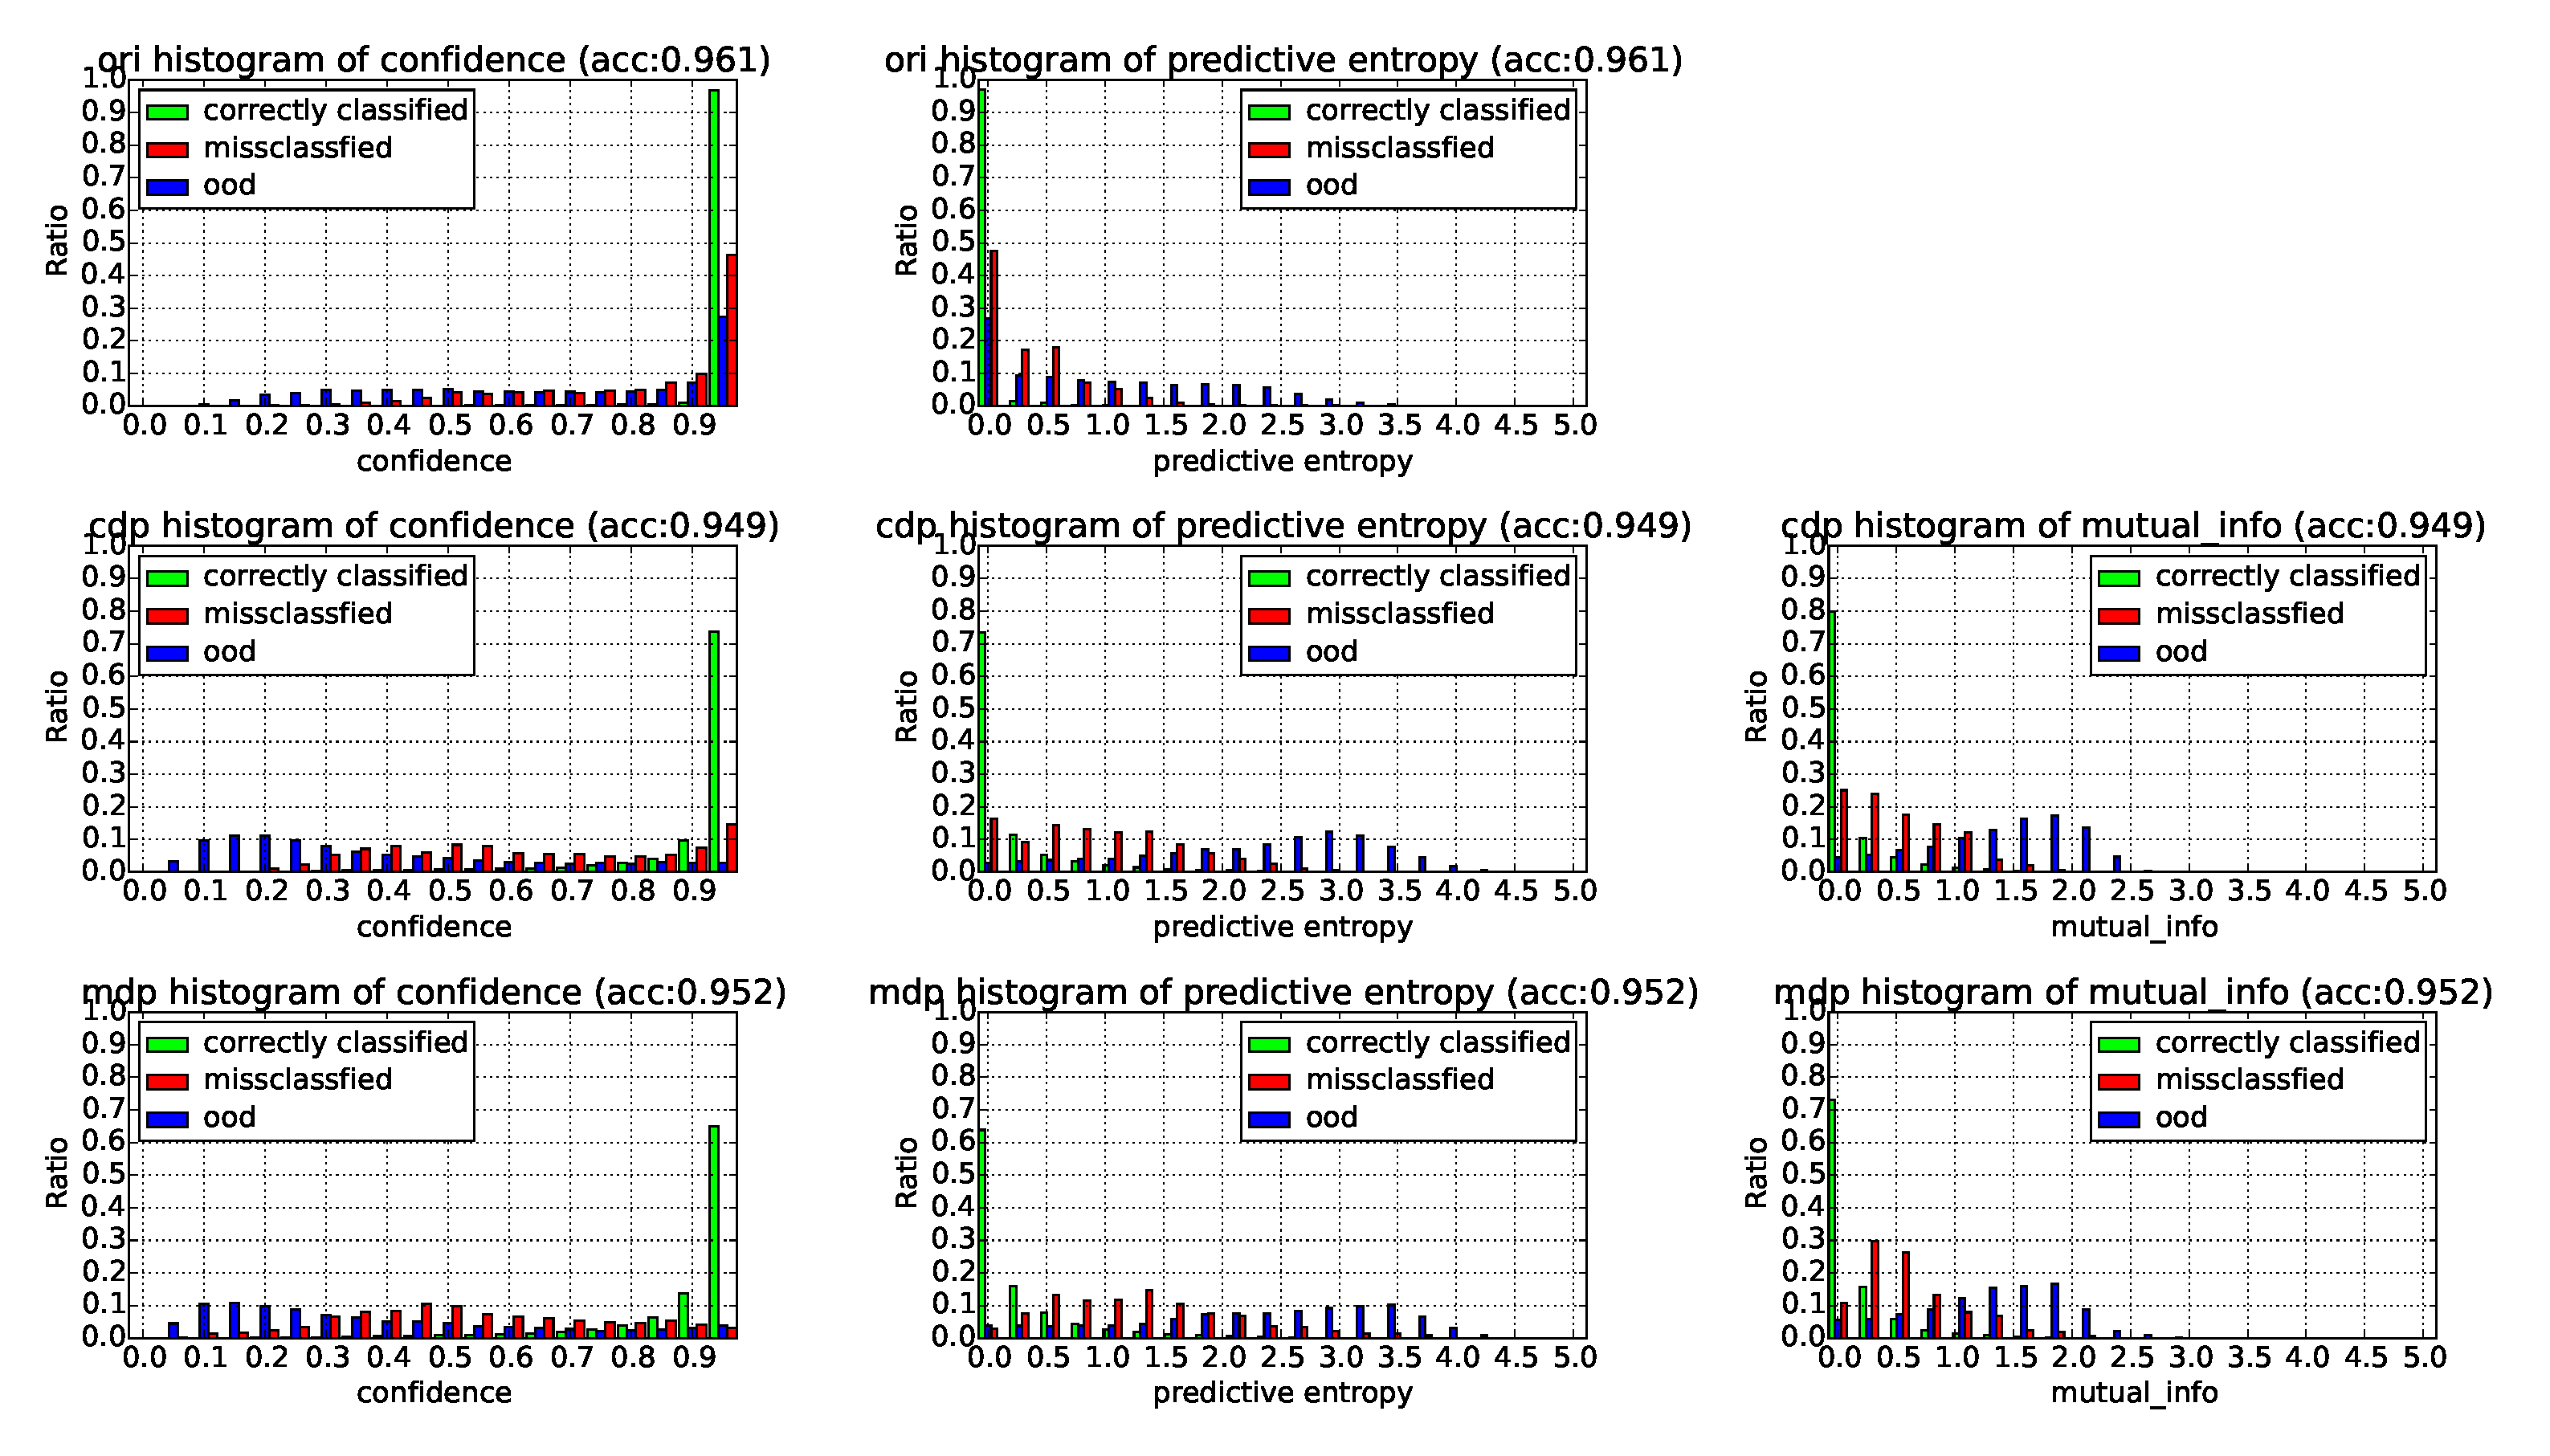
\includegraphics[height=8cm, width=15cm]{uncertainty_estimation/exp1/exp1_histo}
		\caption{Uncertainty(confidence, predictive entropy, mutual information) histograms of original ResNet50, ResNet50 with concrete dropout and ResNet50 with multi-dropout.}		
		\label{exp1_histo}
	\end{center}
\end{figure}
\begin{figure}[H]
	\begin{center}
		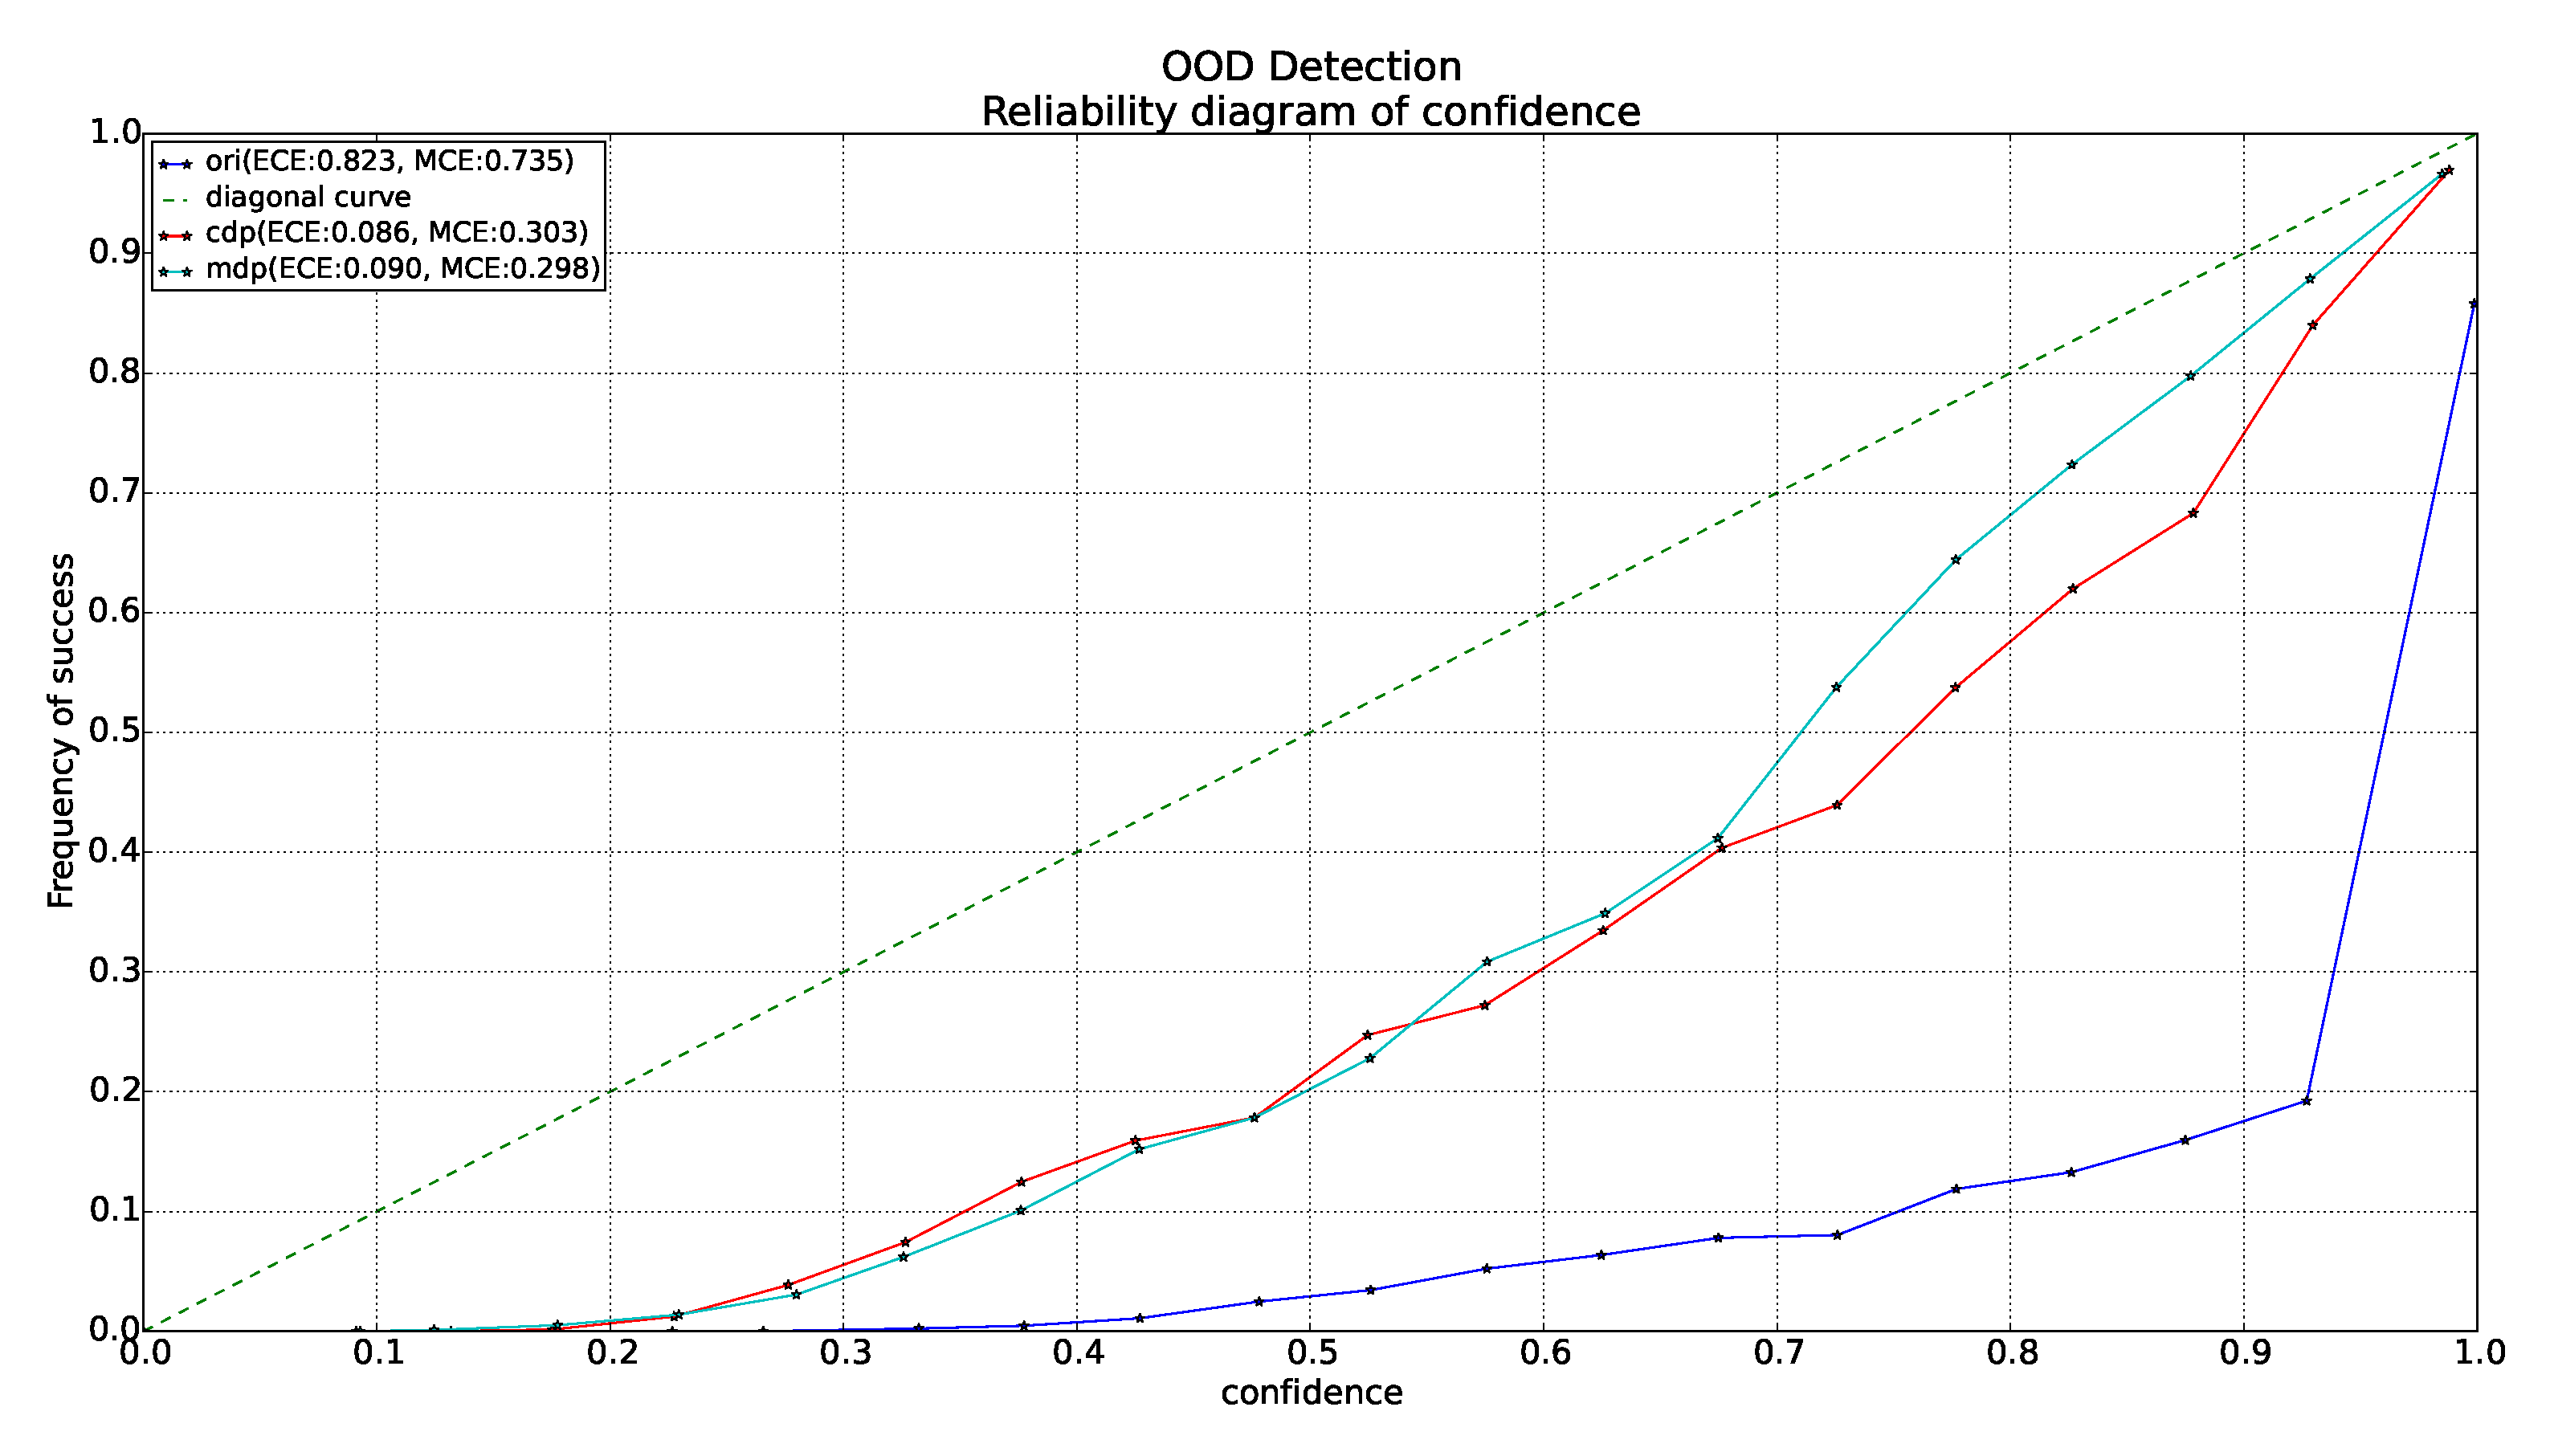
\includegraphics[height=6cm, width=11cm]{uncertainty_estimation/exp1/exp1_reliability}
		\caption{Calibration curves of original ResNet50, ResNet50 with concrete dropout and ResNet50 with multi-dropout evaluated on both test set and OOD dataset.}		
		\label{exp1_reliability}
	\end{center}
\end{figure}

\subsection{Experiments \RNum{2}: uncertainty estimation on category recognition}
In this experiment, we evaluate our model on a category recognition task. The difficulties are expressed in two-fold. Firstly, in this task, the model is confronted with classes with more overlapping. Second, because we want to simulate situation of deploying robots in real world scenario and facing data in real world, the UniHB dataset with domain gap(cf. Fig.\ref{fig:wrgbd2}) to WRGBD is used to achieve this goal. This means, the uncertainty estimation should not only be able to perform well on dataset with exactly same distribution to training set, but also to generalize well to dataset with domain gap which may decrease the accuracy significantly.

Accordingly, we use the entire WRGBD dataset including all view points, whose size is around $\sim$160.9K, to train our model (in which we split off training set for validation set with ratio 2:8). When it comes to UniHB dataset, we treat objects captured in elevation $30^\circ$ and $60^\circ$ in this dataset as \textbf{adaptation set}, whose size is around $\sim$17.1K. We test performance of uncertainty estimation on this adaptation dataset. The images of $45^\circ$, whose size is around $\sim$8.6K , are used for final evaluation after we fine-tune the model with subset of adaptation set to obtain a domain specific model. The latter part will be experimented in next section. Besides, we also evaluate the uncertainty estimation on OOD dataset(cf. Fig.\ref{fig:not_in_wrgbd}) whose size is around $\sim$6.0K. 

We firstly explain protocols in the following for different kinds of metric, which can help understanding the plots and extracting useful information more easily and quickly.  
\begin{itemize}
	\item The following visual metrics are chosen in one of three runs of different random seeds. The average quantitative results are given in tables following the visual metrics.
	\item The calibration curve with title "Classification" on the left is plotted \textbf{only} on predictions of test set. The one with title "OOD detection" on the right is plotted on predictions of \textbf{both} OOD dataset and test dataset.
	\item The ROC curve and PR curve measure the separability between two types of prediction.
	The ones with title "classification" on the left measure the separability between \textbf{correct prediction} and \textbf{miss-classification}. The ones with title "OOD detection" on the right measure the separability between \textbf{correct prediction} and \textbf{OOD prediction}. In all ROC curve and PR curve, correct prediction is always chosen to be positive.
	\item As is shown in uncertainty histogram, we have used three uncertainty measures. Each one has its own ROC curve and PR curve of correct prediction versus miss-classification or OOD prediction. In the following plots of ROC curve and PR curve, we only show the one with highest area under curve. In detail, \textbf{Confidence} is chosen in case of correct prediction versus miss-classification. \textbf{Mutual information} is chosen in case of correct prediction versus OOD prediction.
\end{itemize}   

\subsubsection{Comparison with Ensemble}
In this subsection, we will show the results in not only a qualitative (visual) way, but also in a quantitative way. The approaches we compare here include original version of ResNet50(ori), modified ResNet50 with concrete dropout(cdp), modified ResNet50 with multiple dropout(mdp) as well as their ensemble version. The members in ensemble are just initialized from different random seeds and no other techniques for enhancing the performance are used. In order to quantify the results more objectively, we average the results from three different random seeds and report the mean and the standard deviation.

In the Fig.\ref{exp2_reliability}, on the left there are calibration curves of different approaches, plotted from predictions on test dataset. We can see that the calibration performance is improved a lot by the cdp and mdp. Additionally, their ensemble versions can give even better results which are tightly overlapping with the diagonal curve. On the right there are curves plotted from predictions on both test dataset and OOD dataset. Similar ranks and trends as the left curves appear here. After adding the OOD data into evaluation, all of the calibration curves are pulled down, which means that the calibration performance get worse. If all OOD data is assigned with low confidence, then curves between left and right should be similar because the accuracy in middle or high confidence interval would not change a lot or be pulled down a lot. By comparison these two figures, we can also see that the robustness against OOD data of cdp, mdp and their ensembles are better than the original version.

In the Fig.\ref{exp2_histo}, we can see uncertainty histograms for different approaches and different uncertainty measures. Firstly, let's compare them vertically. We can see the improvement visually. The original version is still overconfident, which express low uncertainty to more than 50$\%$ of OOD data and nearly 40\% of miss-classification. The  cdp and mdp can lower this percentage to around 10\%, although at the same time the percentage of correct predictions is decreased. But we can know that the predictions for which the model expresses low uncertainty are more likely to be correct. And the ensemble of cdp and mdp can perform even better with miss-classification. However, the ensemble of mdp does not work as well as cdp version on OOD data, which can be seen in the histogram on the last row of the figure. The reason for this will be investigated in a ablation study later. Then we can compare them horizontally, it's shown that different uncertainty measures have similar trends in the histogram. Therefore we need other quantitative metrics for them in order to evaluate different approaches as well as metrics more accurately.  


When it comes to the separability metrics in Fig.\ref{exp2_roc_pr}, as stated before, we measure separability between correct prediction and miss-classification (on the left) and that between correct prediction and OOD prediction (on the right). On separability between correction prediction and miss-classification, cdp, mdp and their ensemble version can improve the results compared with original version in both ROC curve and PR curve on the left. On the other hand, the improvements on separability between correct prediction and OOD data are more obvious on the right. However, as observed before, the ensemble of mdp does not work well with OOD data, which can be observe with this metrics. We can know more from the curves that the worse performance with OOD data in mdp is enlarged by building ensemble of it.    

\begin{figure}[H]
	\begin{center}
		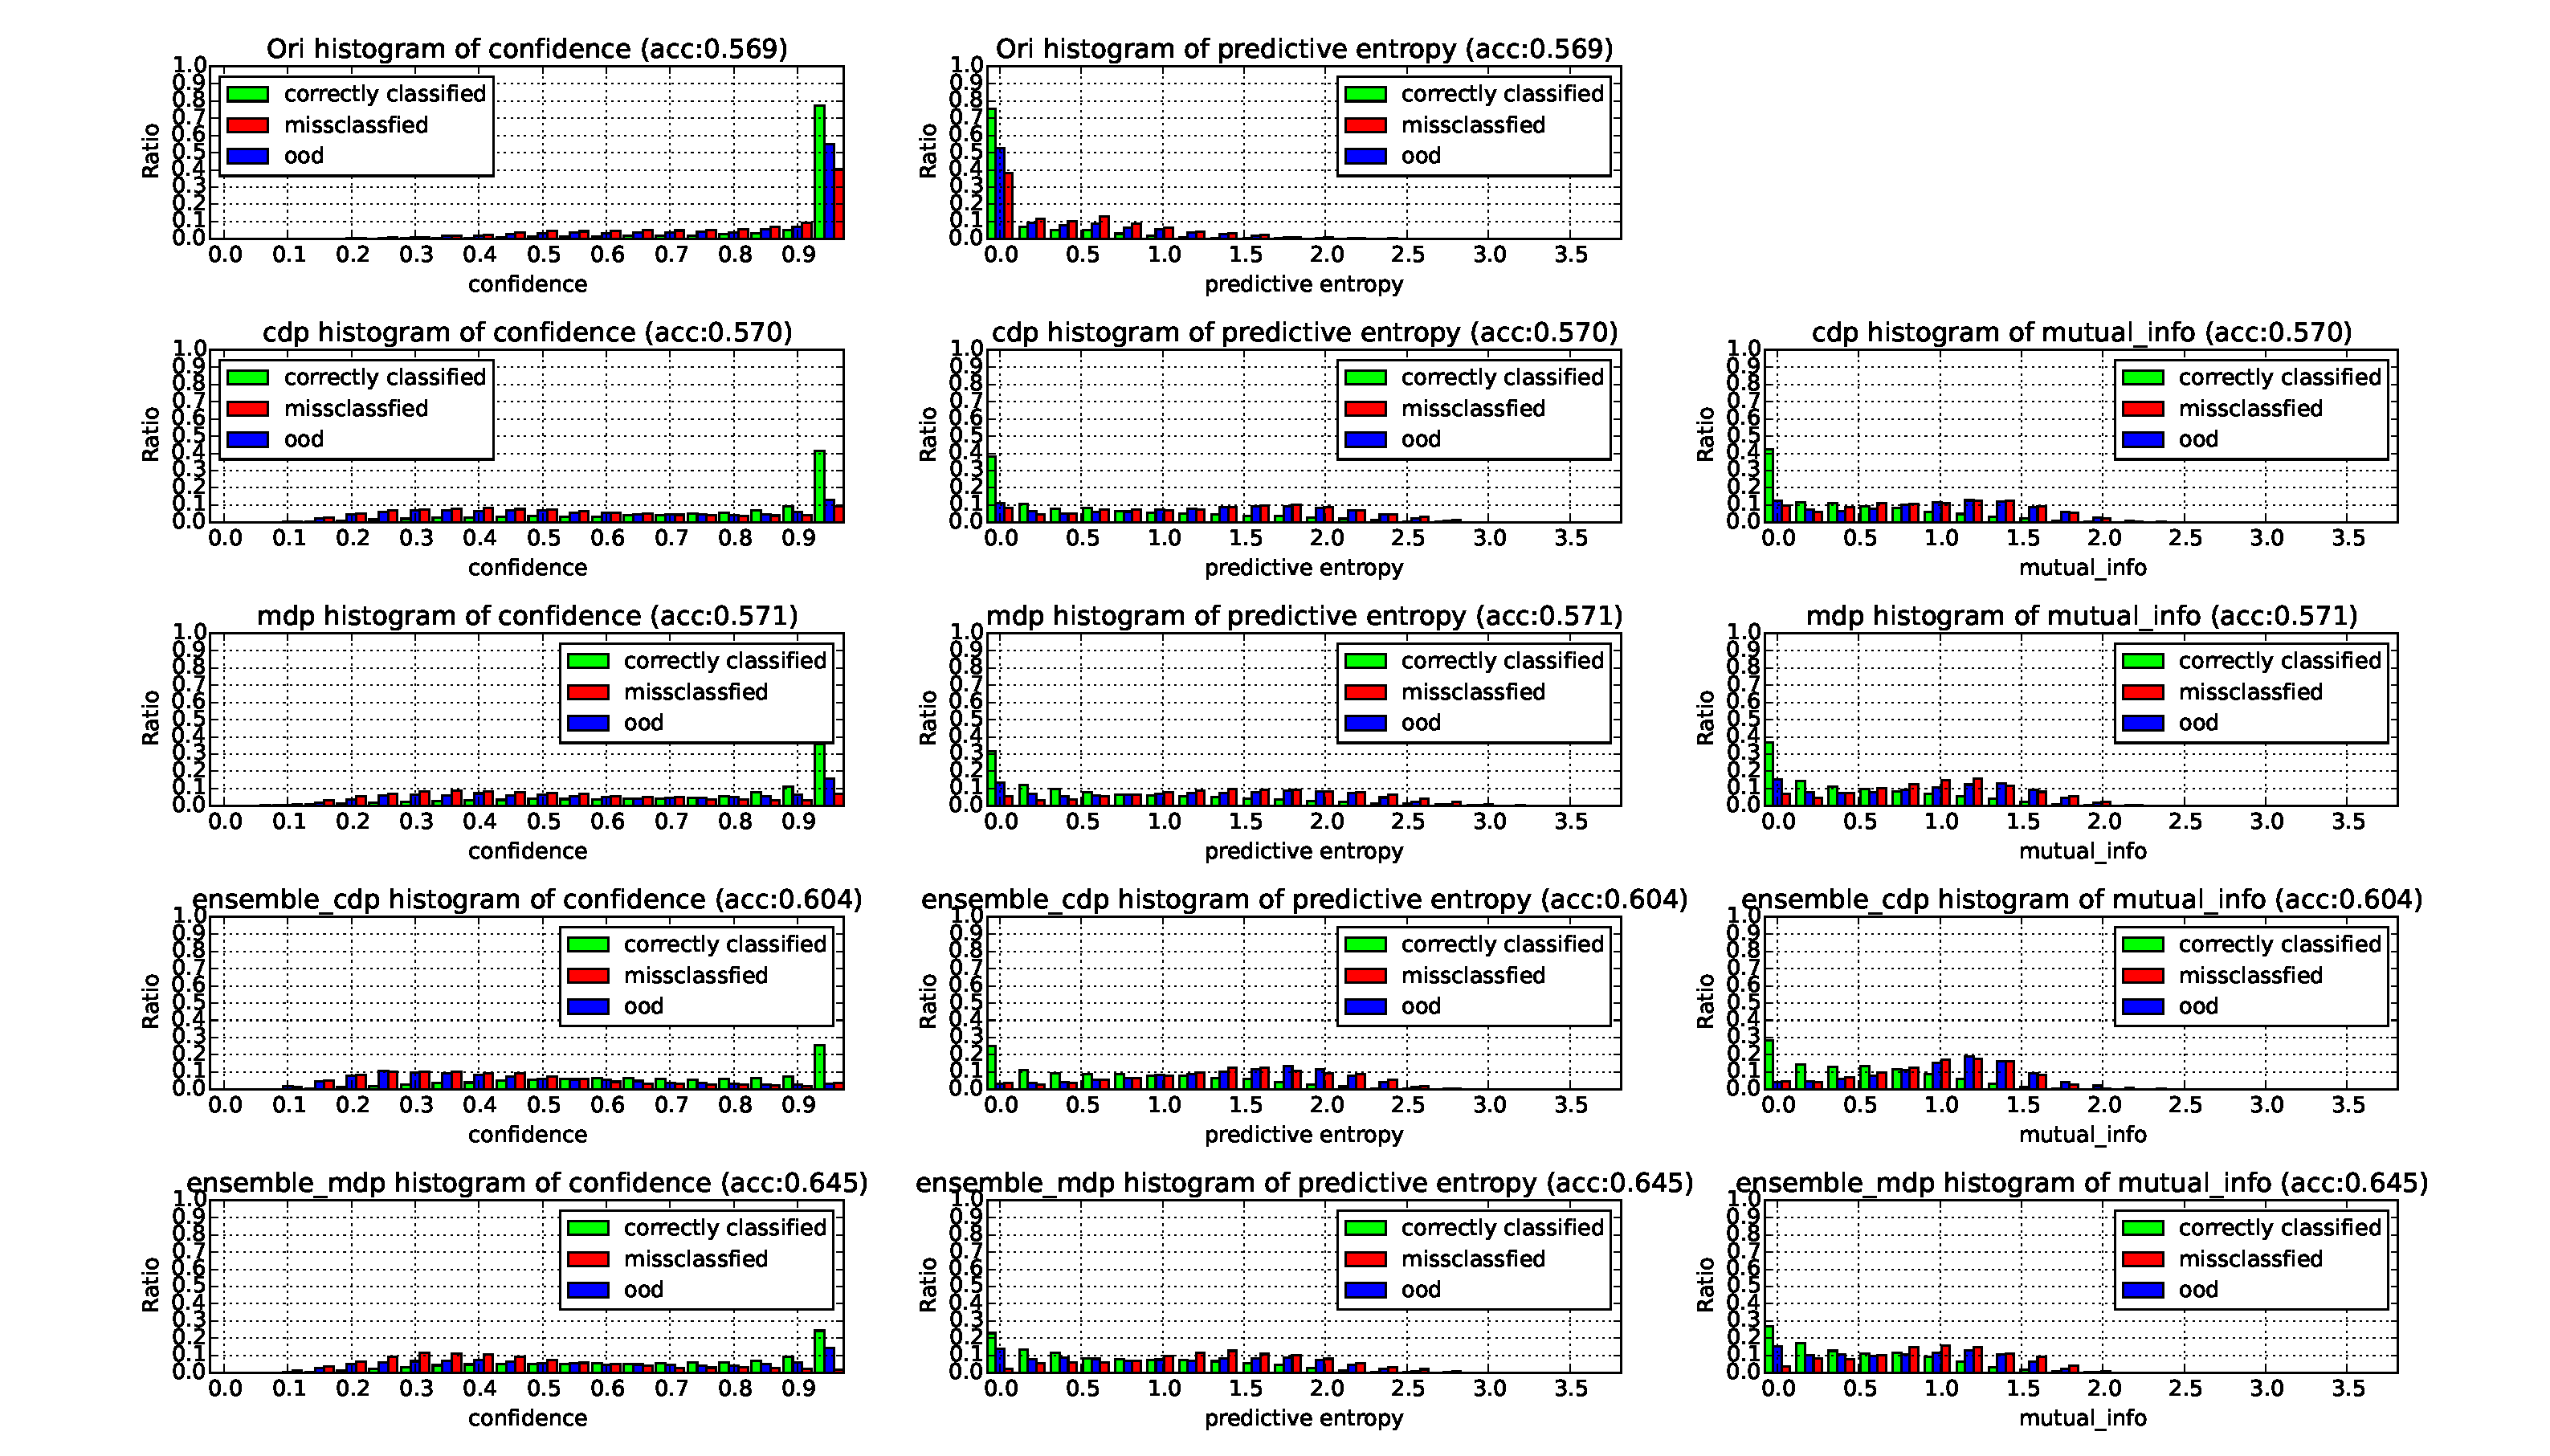
\includegraphics[height=10.5cm, width=16cm]{uncertainty_estimation/hist_seed3_ensemble}
		\caption{Uncertainty histograms of confidence, predictive entropy, mutual information for ori, cdp, mdp, ensemble of cdp, ensemble of mdp in one of three runs.}		
		\label{exp2_histo}
	\end{center}
\end{figure}

\begin{figure}[H]
	\begin{center}
		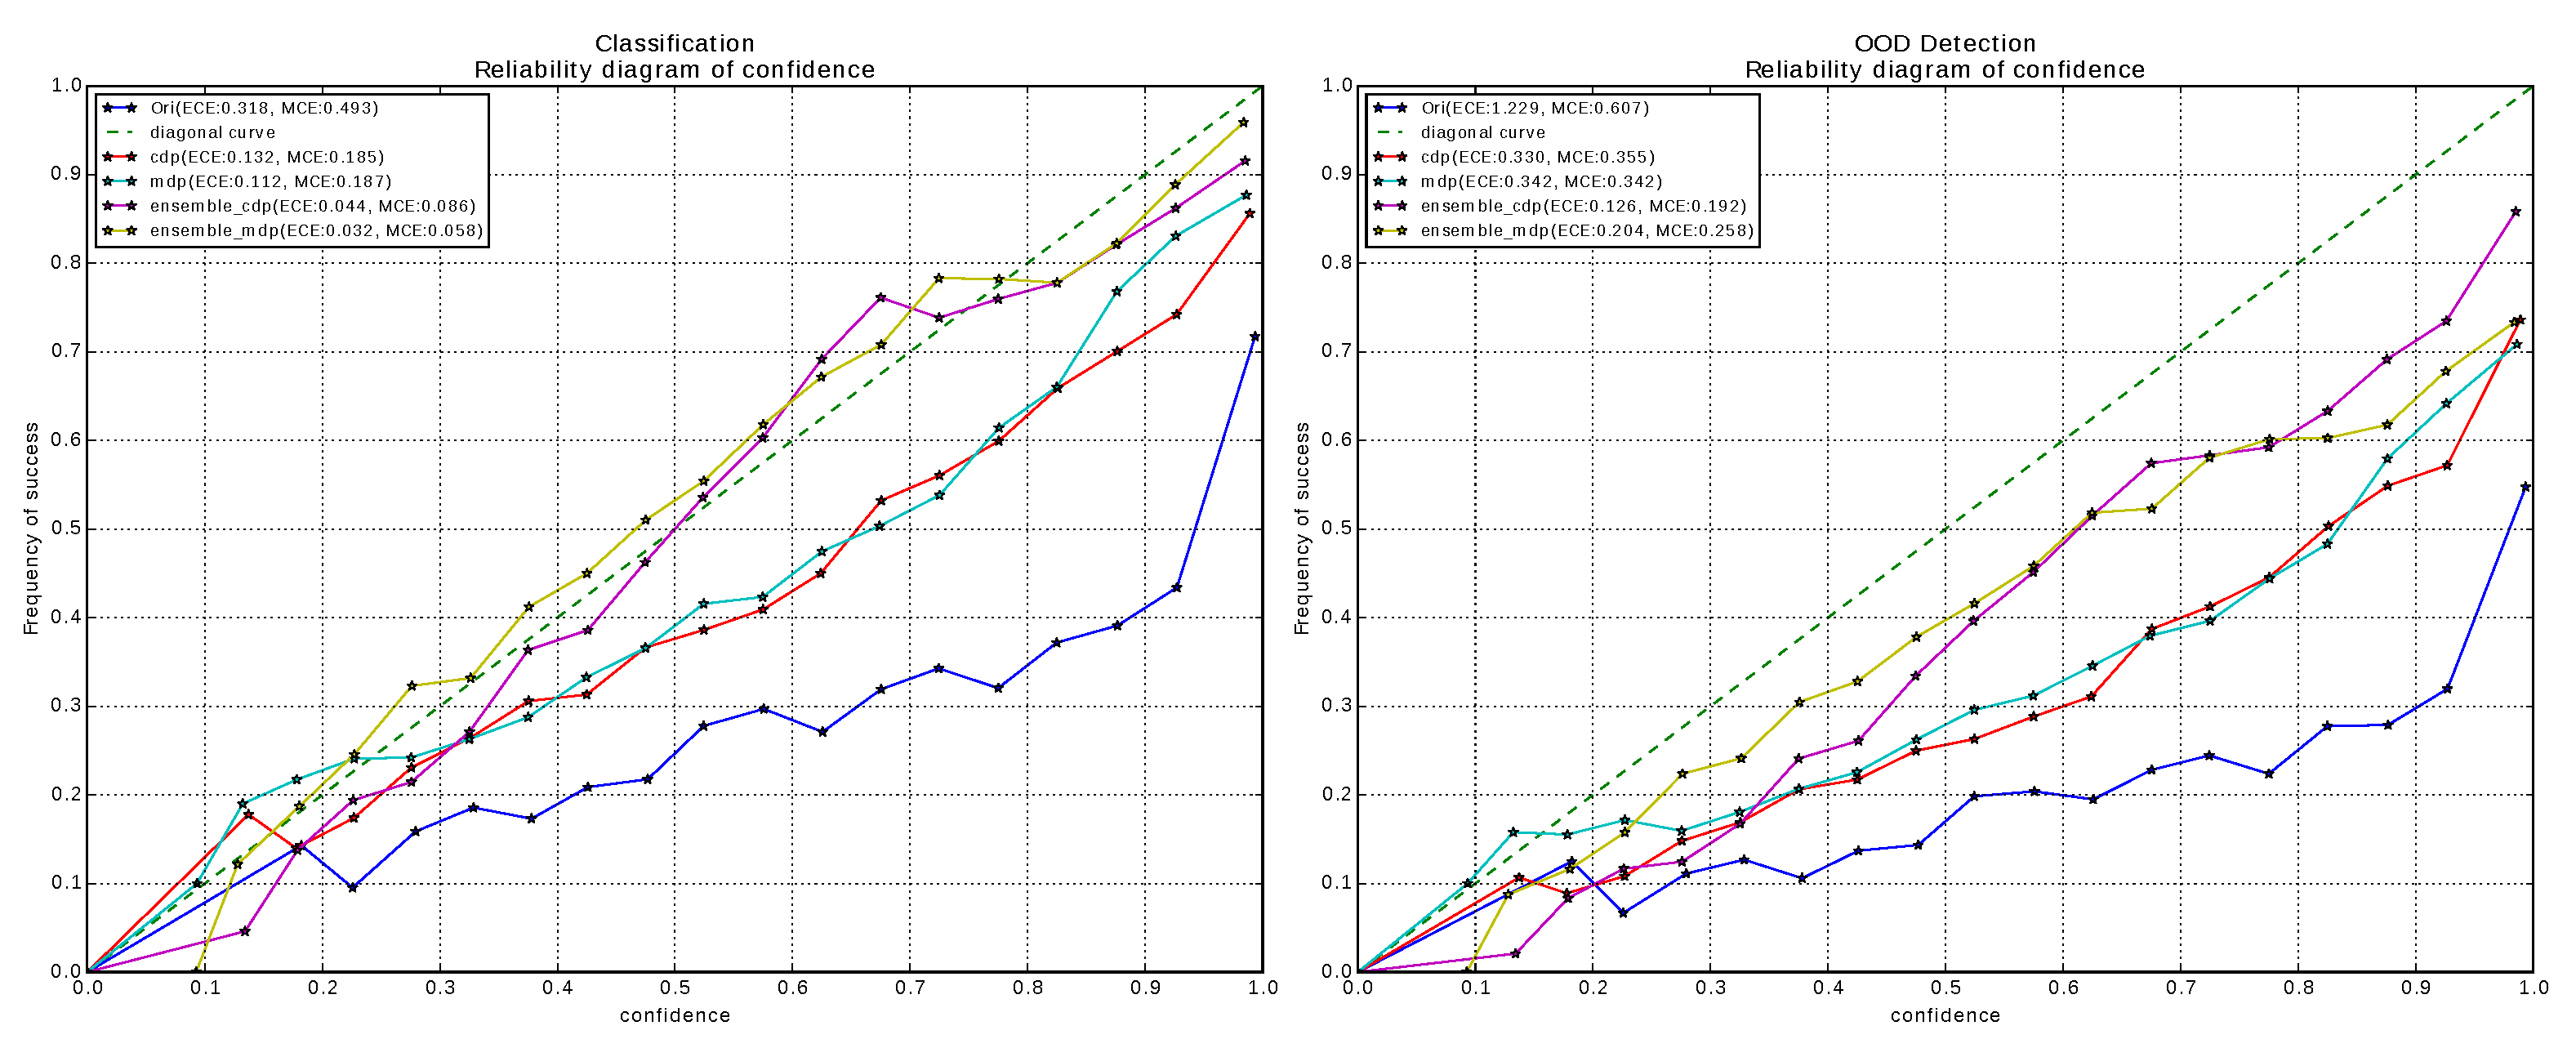
\includegraphics[height=6cm, width=16cm]{uncertainty_estimation/reliability_seed3_ensemble_}
		\caption{Calibration curve for ori, cdp, mdp, ensemble of cdp, ensemble of mdp in one of three runs.}		
		\label{exp2_reliability}
	\end{center}
\end{figure}

\begin{figure}[H]
	\begin{center}
		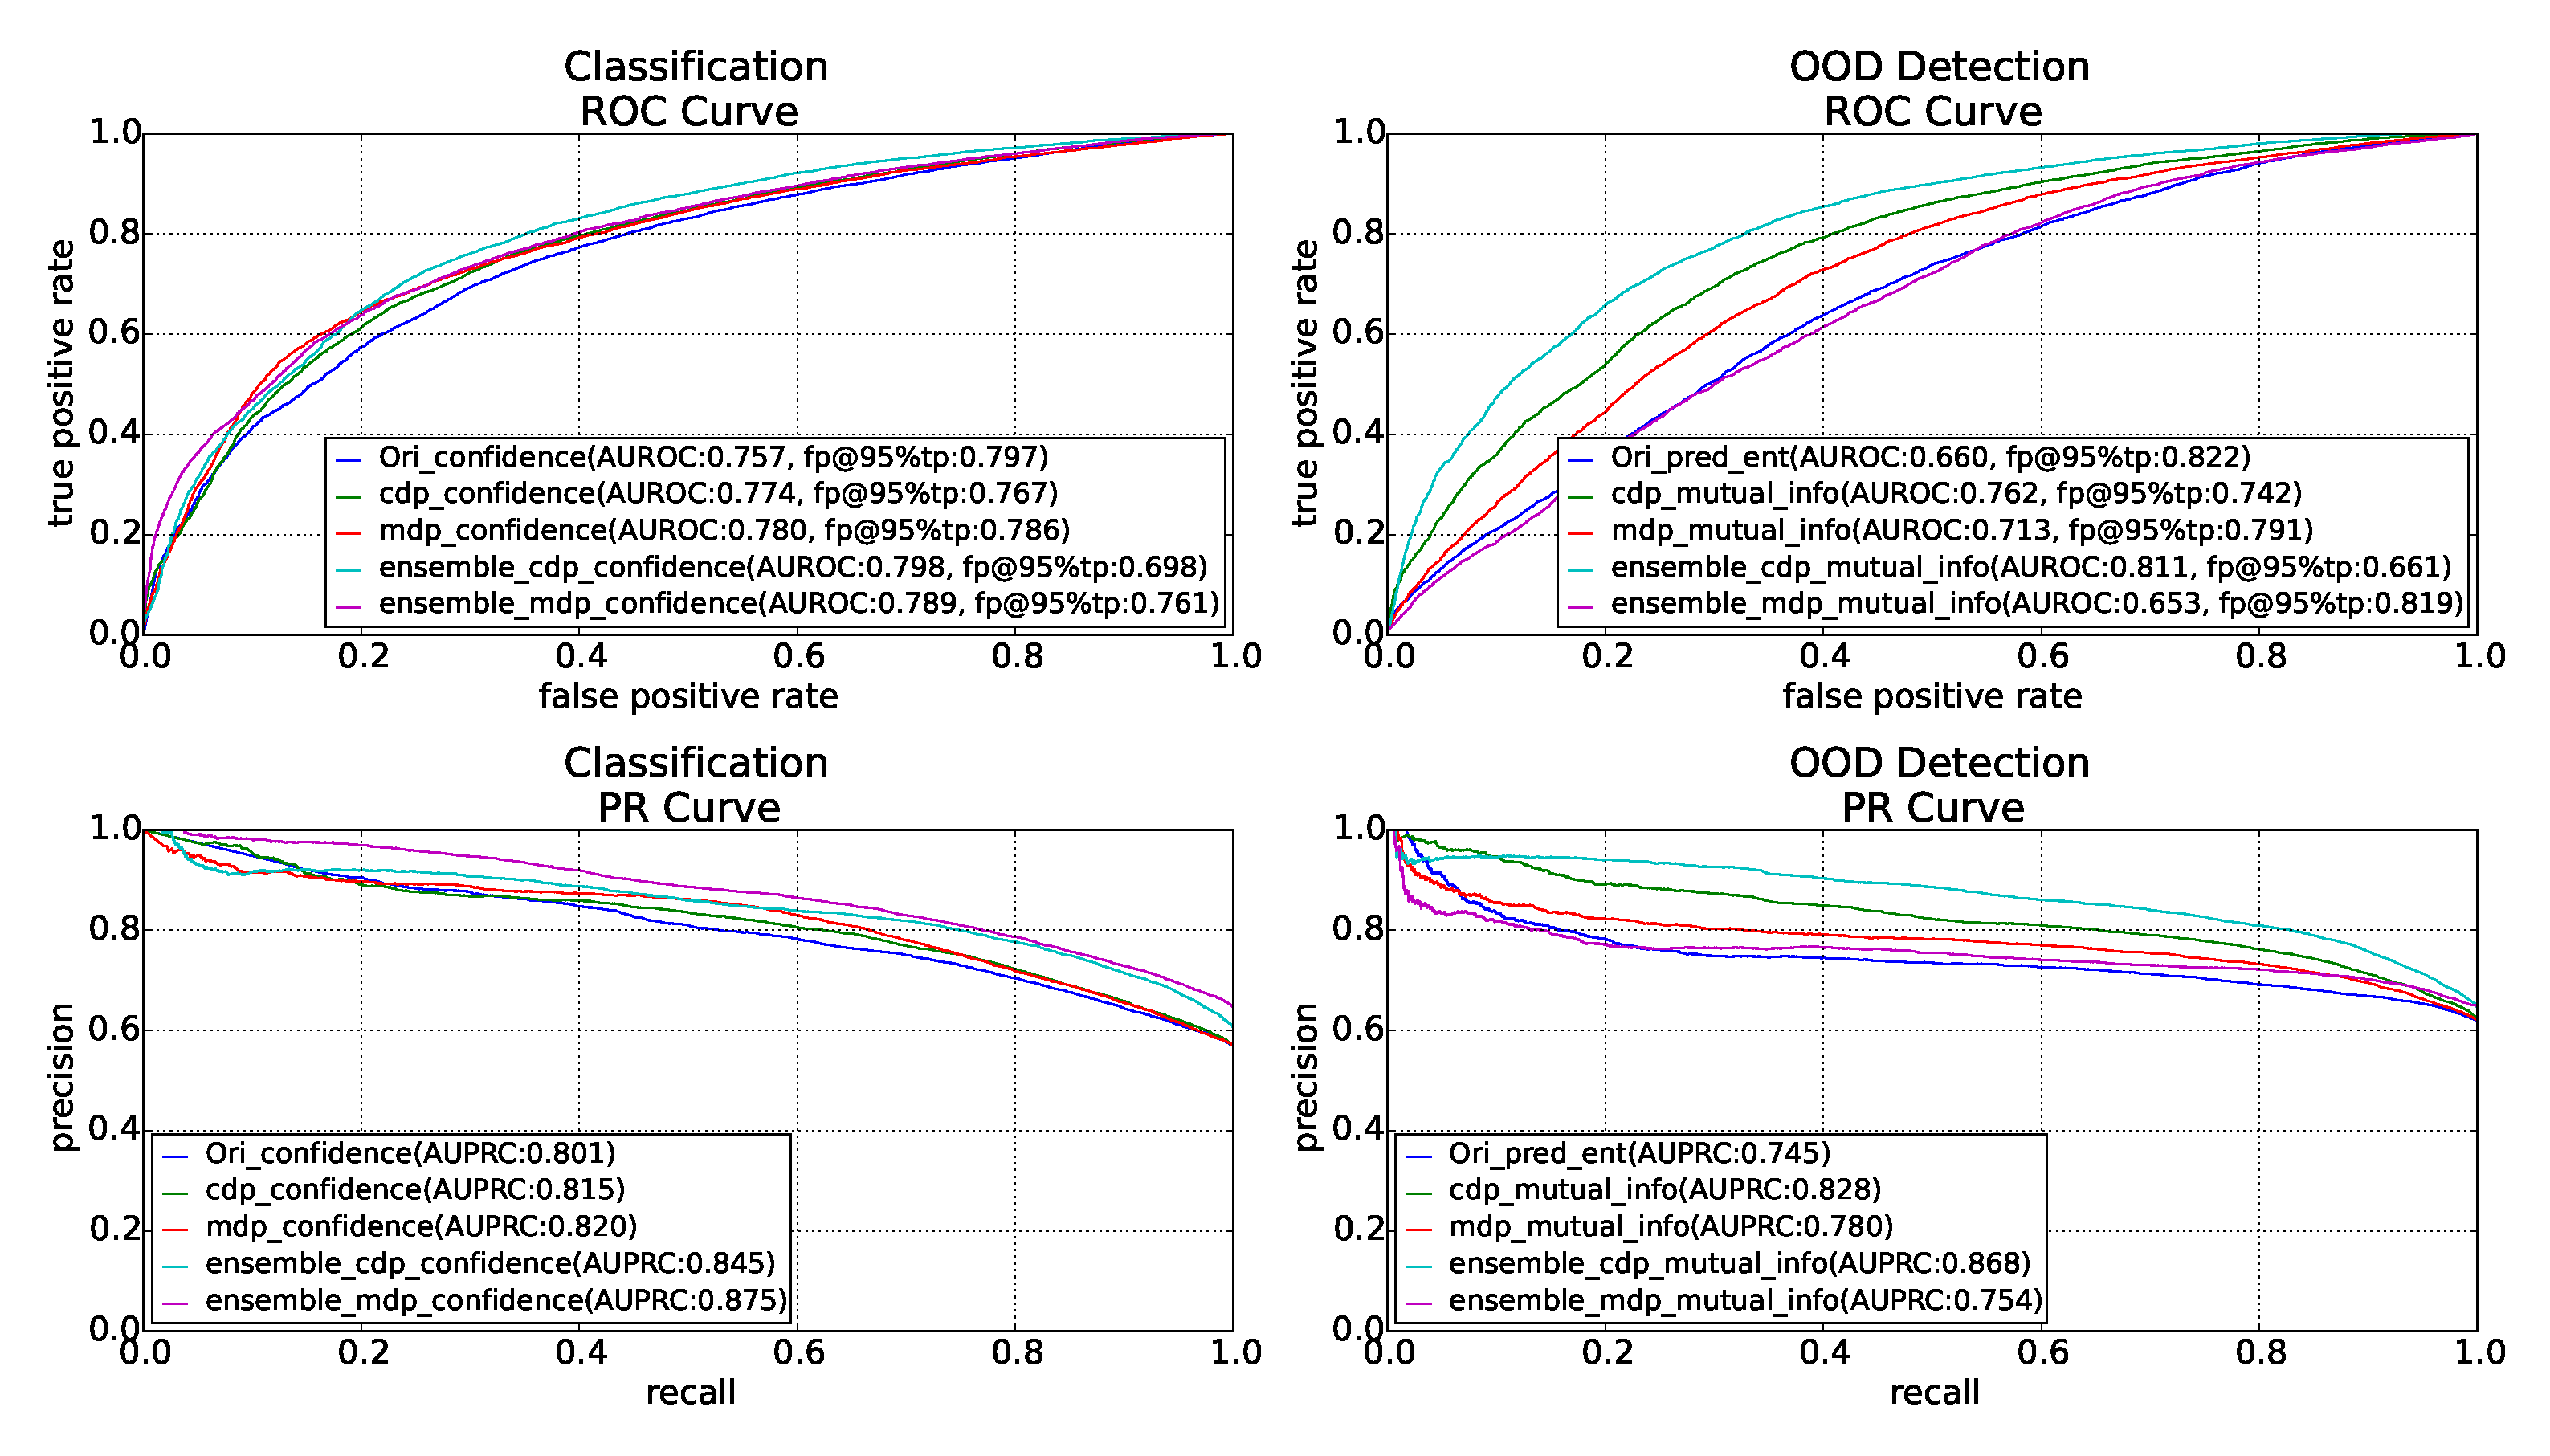
\includegraphics[height=9.5cm, width=16cm]{uncertainty_estimation/roc_pr_seed3_ensemble}
		\caption{ROC and PR curve of ori, cdp, mdp, ensemble of cdp, ensemble in one of three runs.}		
		\label{exp2_roc_pr}
	\end{center} 
\end{figure}

Before we only show the visual metrics for evaluation, it's better to quantify the performance quantitatively. We adopt different aforementioned metrics to achieve this which are presented in the following table \ref{table:compareWithEnsemble}. In order to exclude the influence of random initialization, we train three models of different random seeds and report the mean and standard deviation for each metric. We can see the improvements by cdp, mdp and their ensemble versions along all the metrics. The phenomenon that mdp does not work well with OOD and this effect enlarged by ensemble is also expressed in the table. Based on these experiment results, we can draw the conclusion that, concrete dropout and multiple dropout can improve both accuracy and calibration performance compared with original ResNet50. While the ensemble of concrete dropout and multiple dropout work even better without OOD data, the ensemble of multiple dropout work worse than that of concrete dropout when considering OOD data in this work. When comparing concrete dropout and multiple dropout, concrete dropout is more robust than multiple dropout because the latter one does not work well with OOD data.

\begin{table}[H]
	\centering
	\caption{Quantitative results of acc, bs, nll, ece, mce, auroc, aupr averaged from 3 different random seeds}
	\begin{tabular}{|l|l|l|l|}
		\hline
		& accuracy$ \boldsymbol\uparrow$     & brier\_score $ \boldsymbol \downarrow$& \begin{tabular}[c]{@{}l@{}}negative\\ log \\ likelihood $ \boldsymbol\downarrow$\end{tabular} \\ \hline
		ori           & 0.568$\pm$0.008 & 0.722$\pm$0.019 & 3.242$\pm$0.340                                                         \\ \hline
		cdp           & 0.577$\pm$0.008 & 0.594$\pm$0.013 & 2.088$\pm$0.181                                                         \\ \hline
		mdp           & 0.599$\pm$0.023 & 0.566$\pm$0.020 & 1.940$\pm$0.064                                                         \\ \hline
		emsemble\_cdp & 0.604        & 0.534        & 1.452                                                                \\ \hline
		emsemble\_mdp & \textbf{0.645}        & \textbf{0.496}        & \textbf{1.389}                                                                \\ \hline
	\end{tabular}
\label{table:compareWithEnsemble}
\end{table}

\begin{table}[H]
	\centering
	% \caption{results of ece, mce, auroc, aupr}
	\begin{tabular}{|l|l|l|l|l|}
		\hline
		& \begin{tabular}[c]{@{}l@{}}expected\\ calibration\\ error(w/o. OOD/\\ w. OOD)$ \boldsymbol\downarrow$\end{tabular} & \begin{tabular}[c]{@{}l@{}}maximal\\ calibration\\ error(w/o. OOD/\\ w. OOD)$ \boldsymbol\downarrow$\end{tabular} & \begin{tabular}[c]{@{}l@{}}area under\\ ROC\\ (vs. Miss-\\ classified/\\ vs. OOD)$ \boldsymbol\uparrow$\end{tabular} & \begin{tabular}[c]{@{}l@{}}area under\\ PR curve\\ (vs. Miss-\\ classified/\\ vs. OOD)$ \boldsymbol\uparrow$\end{tabular} \\ \hline
		ori           & \begin{tabular}[c]{@{}l@{}}0.304$\pm$0.016 /\\ 0.633$\pm$0.065\end{tabular}                      & \begin{tabular}[c]{@{}l@{}}0.461$\pm$0.027 /\\ 0.362$\pm$0.025\end{tabular}                     & \begin{tabular}[c]{@{}l@{}}0.750$\pm$0.007 /\\ 0.664$\pm$0.011\end{tabular}           & \begin{tabular}[c]{@{}l@{}}0.802$\pm$0.008 /\\ 0.751$\pm$0.018\end{tabular}                \\ \hline
		cdp           & \begin{tabular}[c]{@{}l@{}}0.124$\pm$0.023/\\ 0.288$\pm$0.048\end{tabular}                         & \begin{tabular}[c]{@{}l@{}}0.206$\pm$0.015/ \\ 0.374$\pm$0.018\end{tabular}                     & \begin{tabular}[c]{@{}l@{}}0.775$\pm$0.008/ \\ 0.783$\pm$0.022\end{tabular}           & \begin{tabular}[c]{@{}l@{}}0.825$\pm$0.007/ \\ 0.850$\pm$0.022\end{tabular}                \\ \hline
		mdp           & \begin{tabular}[c]{@{}l@{}}0.114$\pm$0.012/ \\ 0.383$\pm$0.046\end{tabular}                      & \begin{tabular}[c]{@{}l@{}}0.199$\pm$0.016/ \\ 0.367$\pm$0.023\end{tabular}                     & \begin{tabular}[c]{@{}l@{}}0.780$\pm$0.011/ \\ 0.709$\pm$0.004\end{tabular}           & \begin{tabular}[c]{@{}l@{}}0.838$\pm$0.013/ \\ 0.788$\pm$0.006\end{tabular}                \\ \hline
		emsemble\_cdp & \begin{tabular}[c]{@{}l@{}}0.044/\\ \textbf{0.042} \end{tabular} 
		 &  \begin{tabular}[c]{@{}l@{}}0.086/\\\textbf{0.093} \end{tabular}                                                                                    & \begin{tabular}[c]{@{}l@{}}\textbf{0.798}/\\\textbf{0.811}  \end{tabular}                                                                           & \begin{tabular}[c]{@{}l@{}}0.845/\\\textbf{0.868}  \end{tabular}                                                                                \\ \hline
		emsemble\_mdp & \begin{tabular}[c]{@{}l@{}}\textbf{0.032}/\\0.170 \end{tabular}                                                                                       & \begin{tabular}[c]{@{}l@{}}\textbf{0.058}/\\0.227  \end{tabular}                                                                                     & \begin{tabular}[c]{@{}l@{}}0.789/\\0.653 \end{tabular}                                                                            & \begin{tabular}[c]{@{}l@{}}\textbf{0.875}/\\0.754  \end{tabular}                                                                                \\ \hline
	\end{tabular}
\end{table}	

\subsubsection{Comparison with Laplace approximation}
Because Laplace approximation requires only MAP point estimate of model parameter. Therefore we take the already trained model of different approaches as our MAP point estimate and compute the approximation of Kronecker factors with half of training set. We set the scale parameter of Kronecker factors $\sqrt{N}$ as $1$ and dump factor $\sqrt{\tau}$ as $15$ in equation \ref{mvg_prior} based on grid search on the validation set.   

Different visual metrics such histograms, calibration curves, ROC curve and PR curve of cdp, mdp and their Laplace approximation versions are showed in the following. We can see that the Laplace approximation can achieve similar results as the cdp or mdp do in uncertainty histograms, calibration curves as well as ROC curve and PR curve. The histograms of different uncertainty measure show similar trend as before. 

If we compare the Laplace approximation between cdp and mdp, we can see that the result of Laplace approximation is similar to the their dropout versions. This can be observed through that the percentage of OOD prediction with high confidence of Laplace approximation for network trained with mdp is higher than that of Laplace approximation for network trained with cdp in the histogram. Besides, in ROC curve/PR curve on correct prediction vs. OOD data prediction of mdp and cdp, the area under curve of Laplace approximation of mdp is obviously lower than that of cdp. This phenomenon also exists in the histogram and ROC as well as PR curve of mdp and cdp. In the table of quantitative results (cf. \ref{table:lap}), the quantities of different metrics corresponding to the visual metrics. To summarize this, although Laplace can achieve similar results as concrete dropout and multiple dropout do, their performance is highly related to the point estimate of parameter obtained during training.

\begin{figure}[H]		
	\centering
	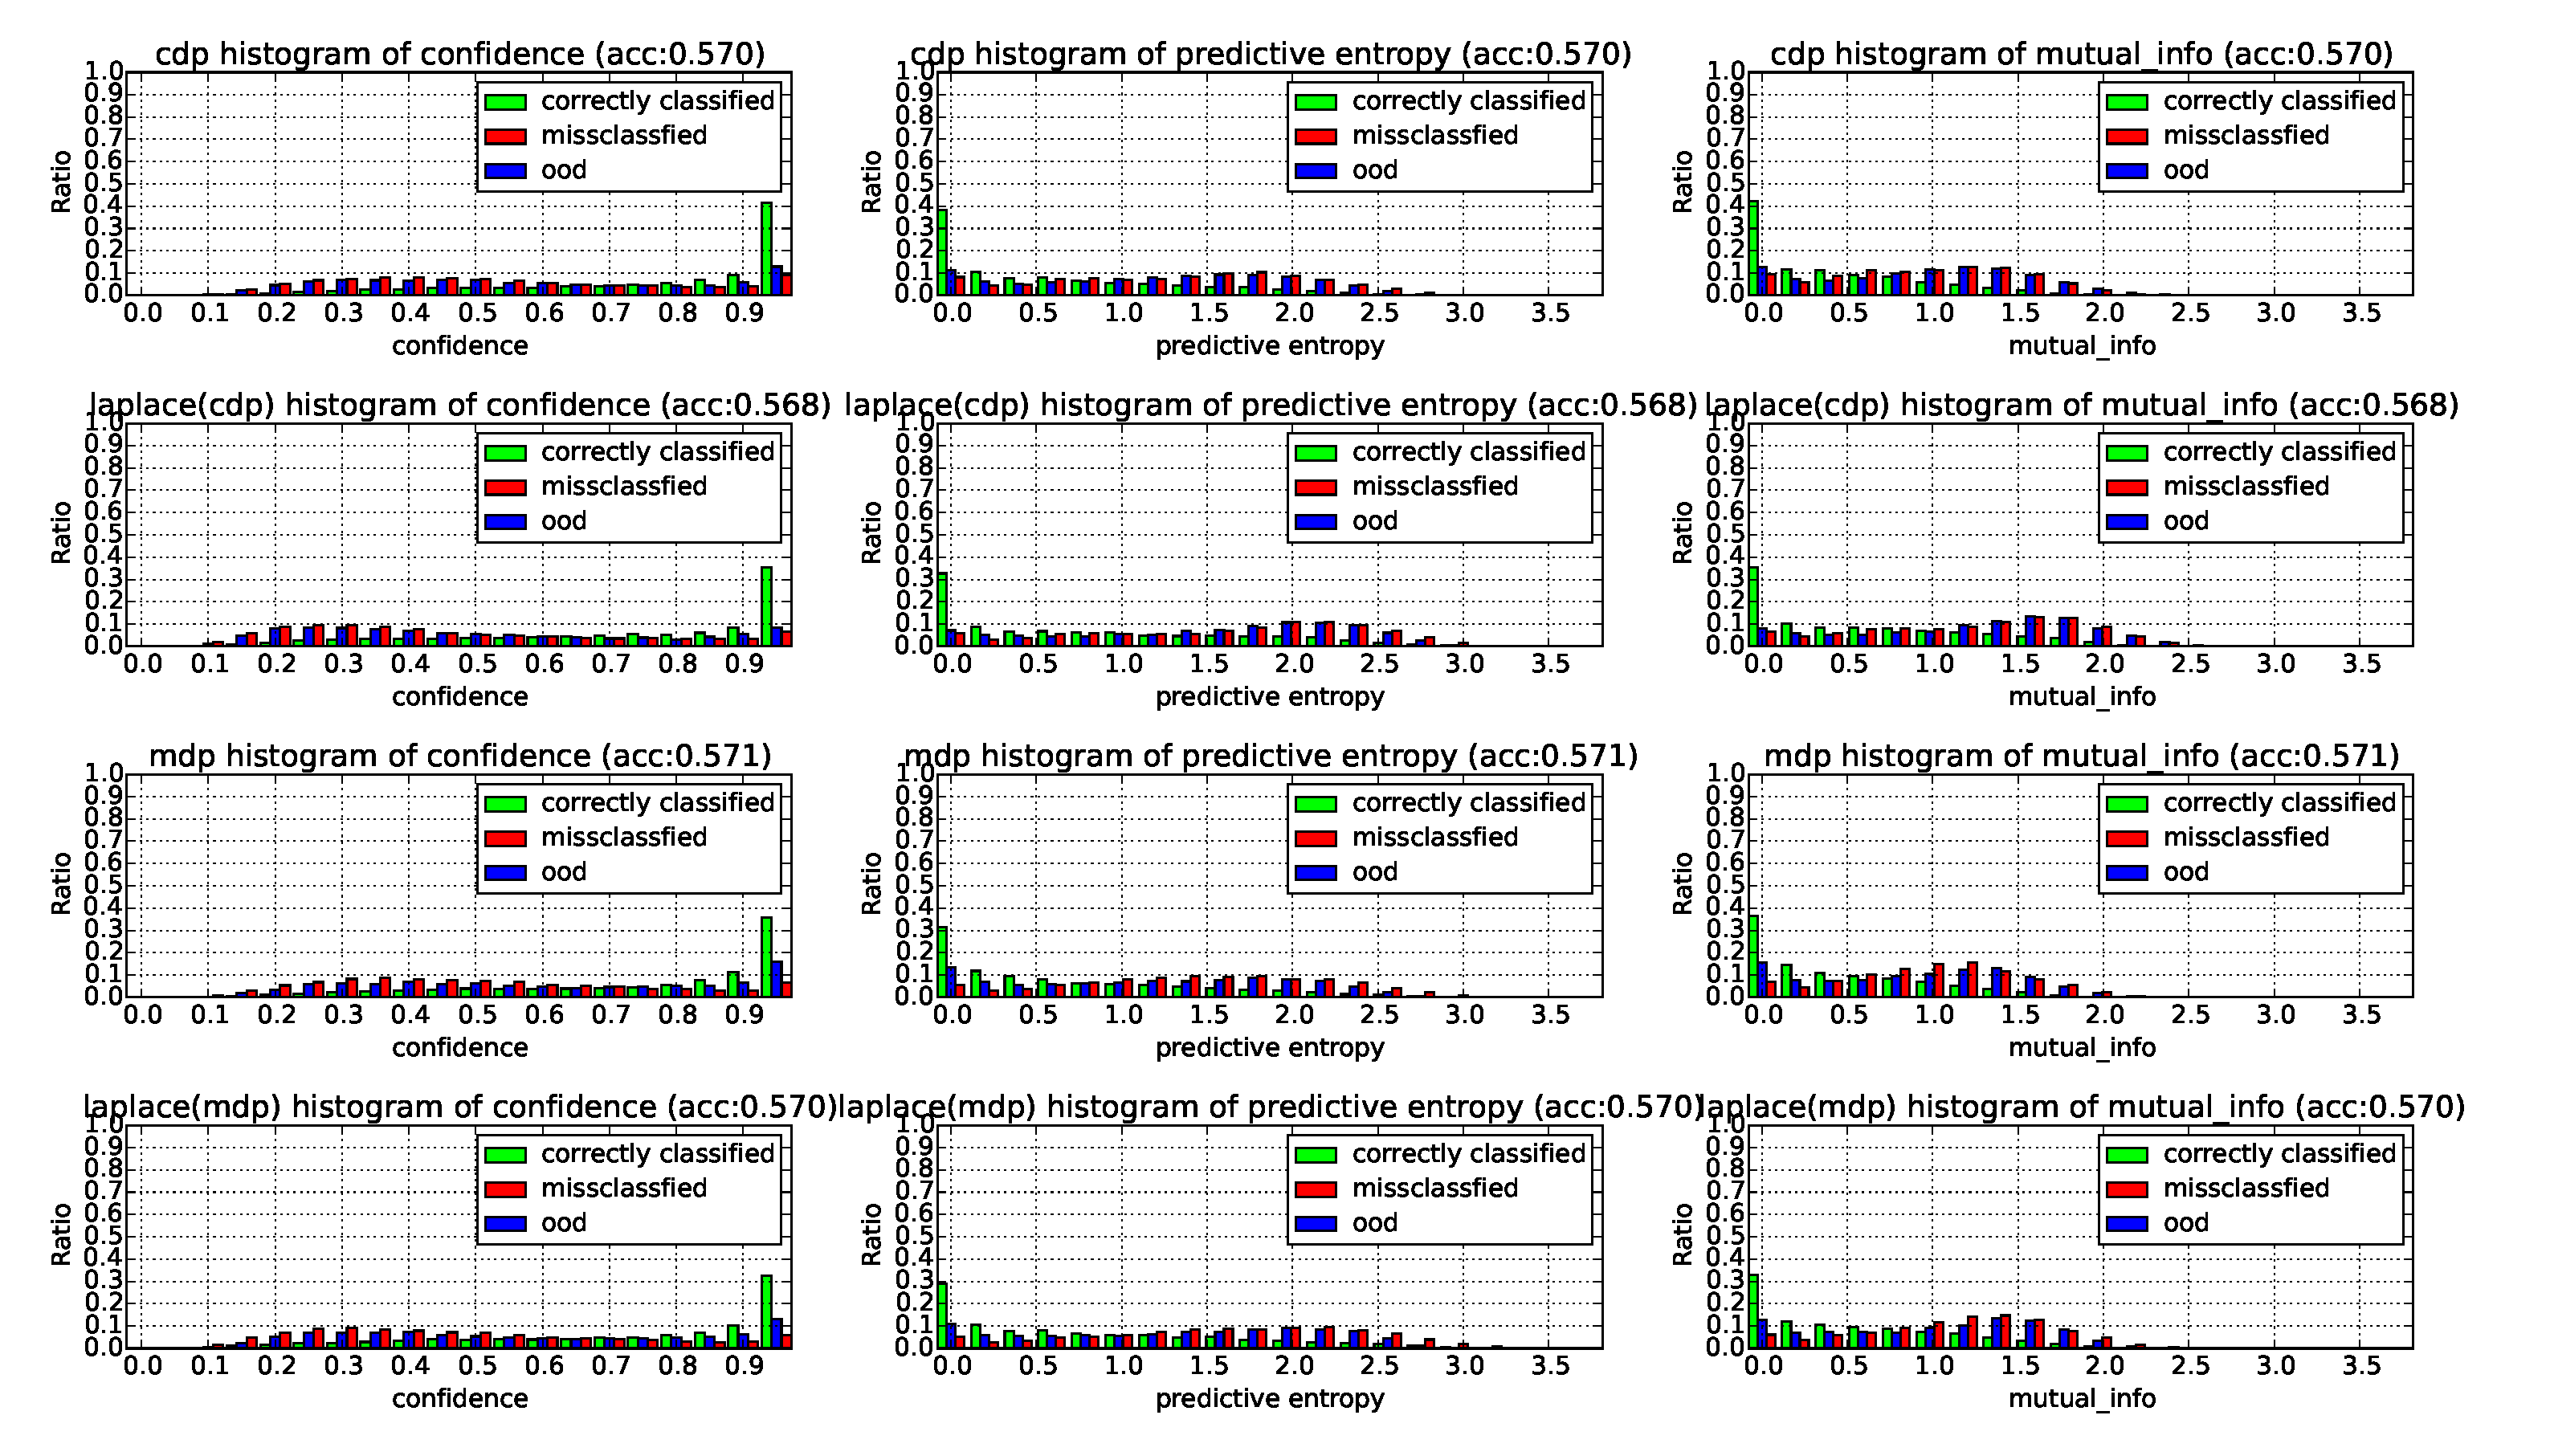
\includegraphics[height=10cm, width=15cm]{uncertainty_estimation/laplace/histo_ood_seed3.eps}
	\caption{Uncertainty histogram of cdp, mdp and their Laplace approximation versions with confidence, predictive entropy and mutual information as uncertainty measure in one of three runs.}
	\label{figure:lap_hist}	
\end{figure}

\begin{figure}[H]
	\begin{center}
		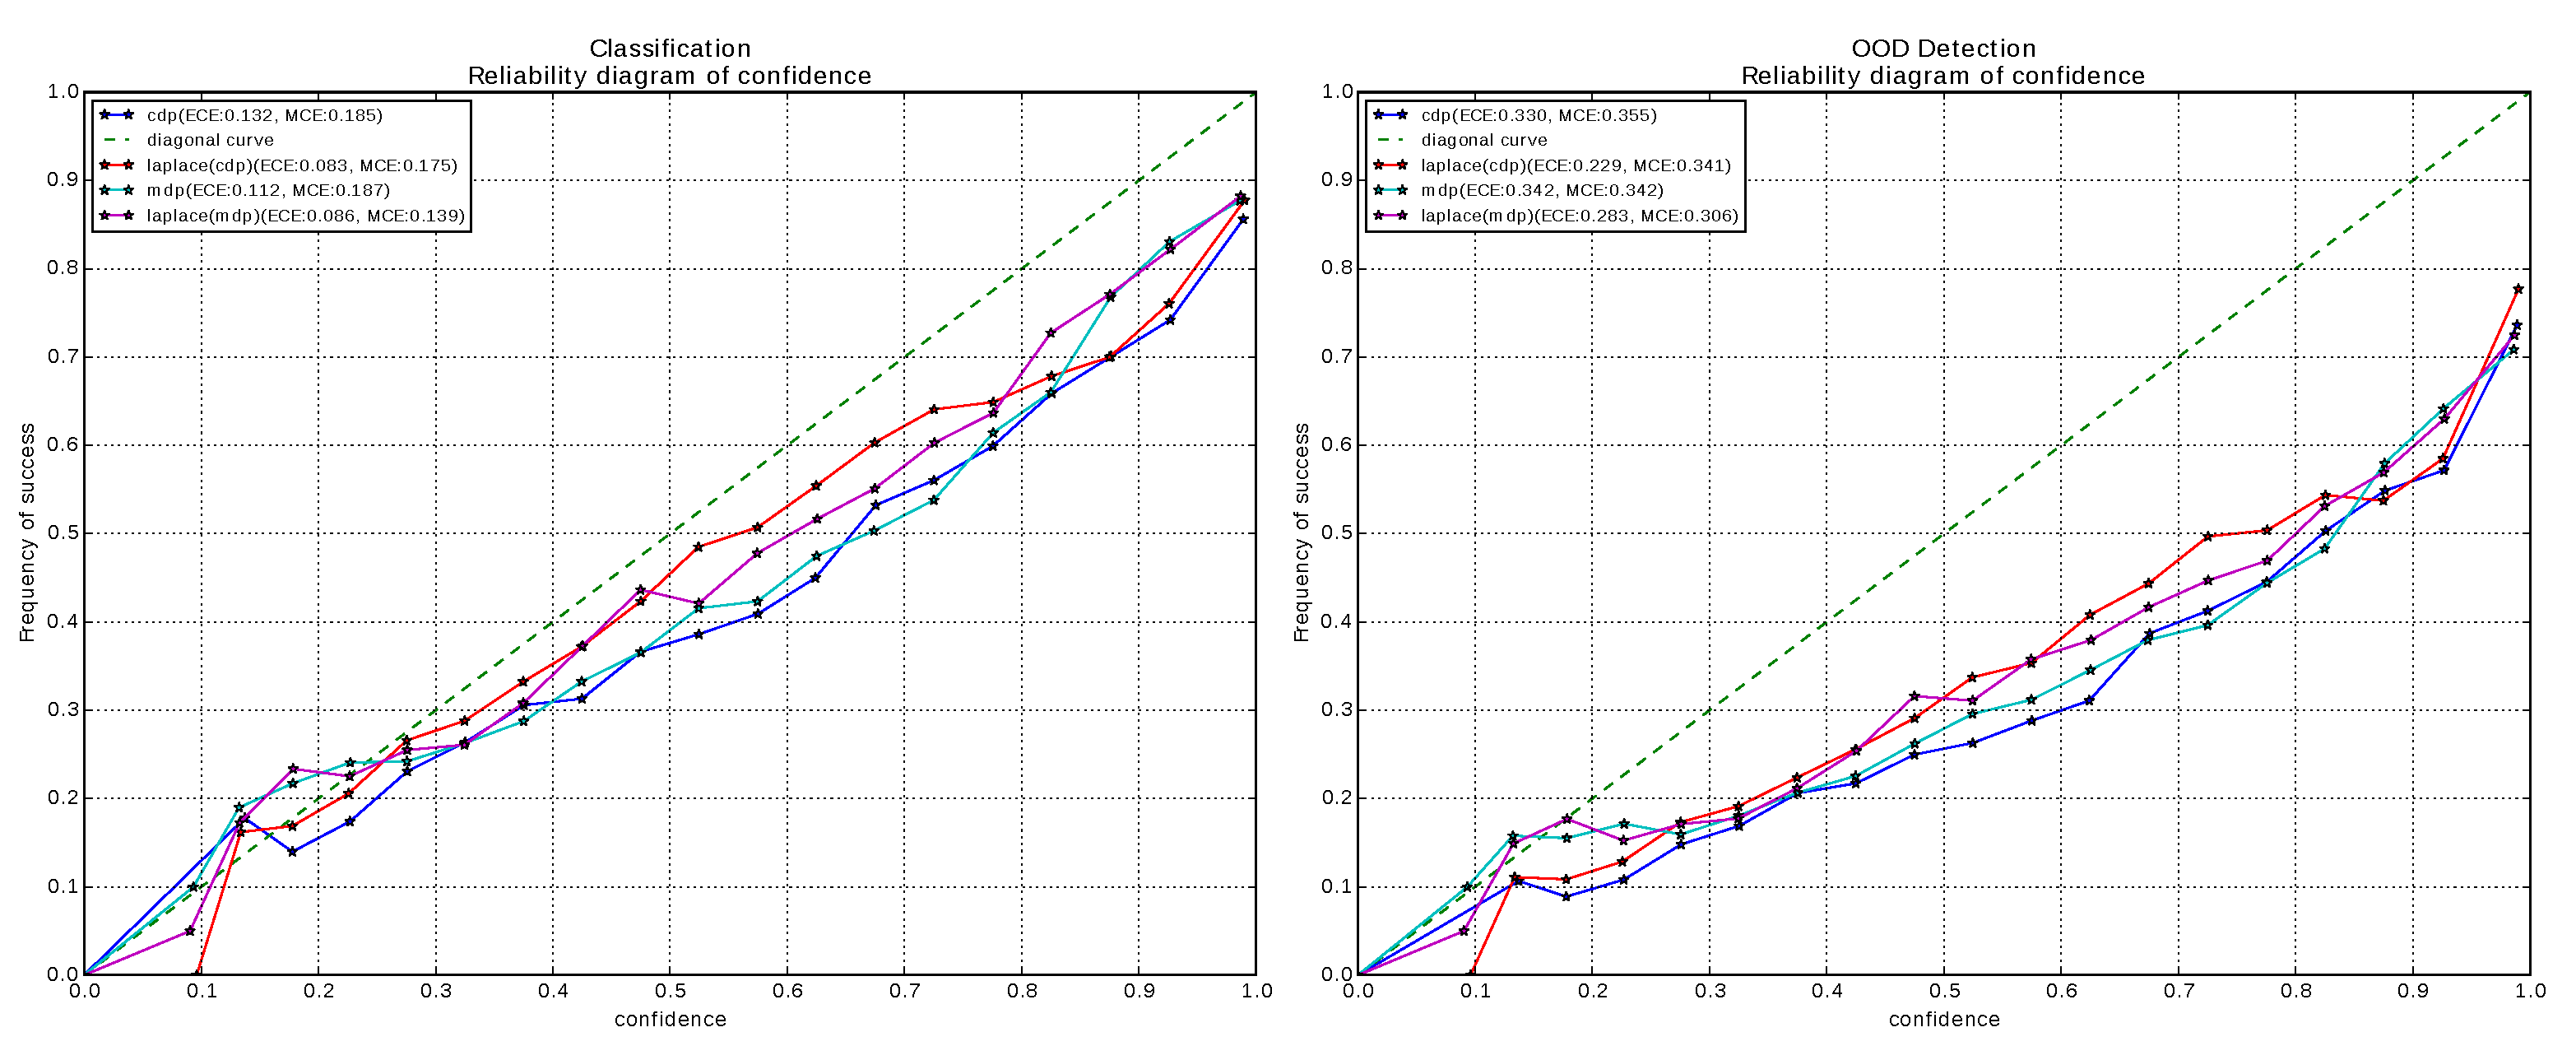
\includegraphics[height=6cm, width=16cm]{uncertainty_estimation/laplace/reliabilty_seed3_.eps}
		\caption{Calibration curve of cdp, mdp and their Laplace approximation versions in one of three runs.}		
		\label{lap_calibration}
	\end{center}
\end{figure}



\begin{figure}[H]
	\begin{center}
		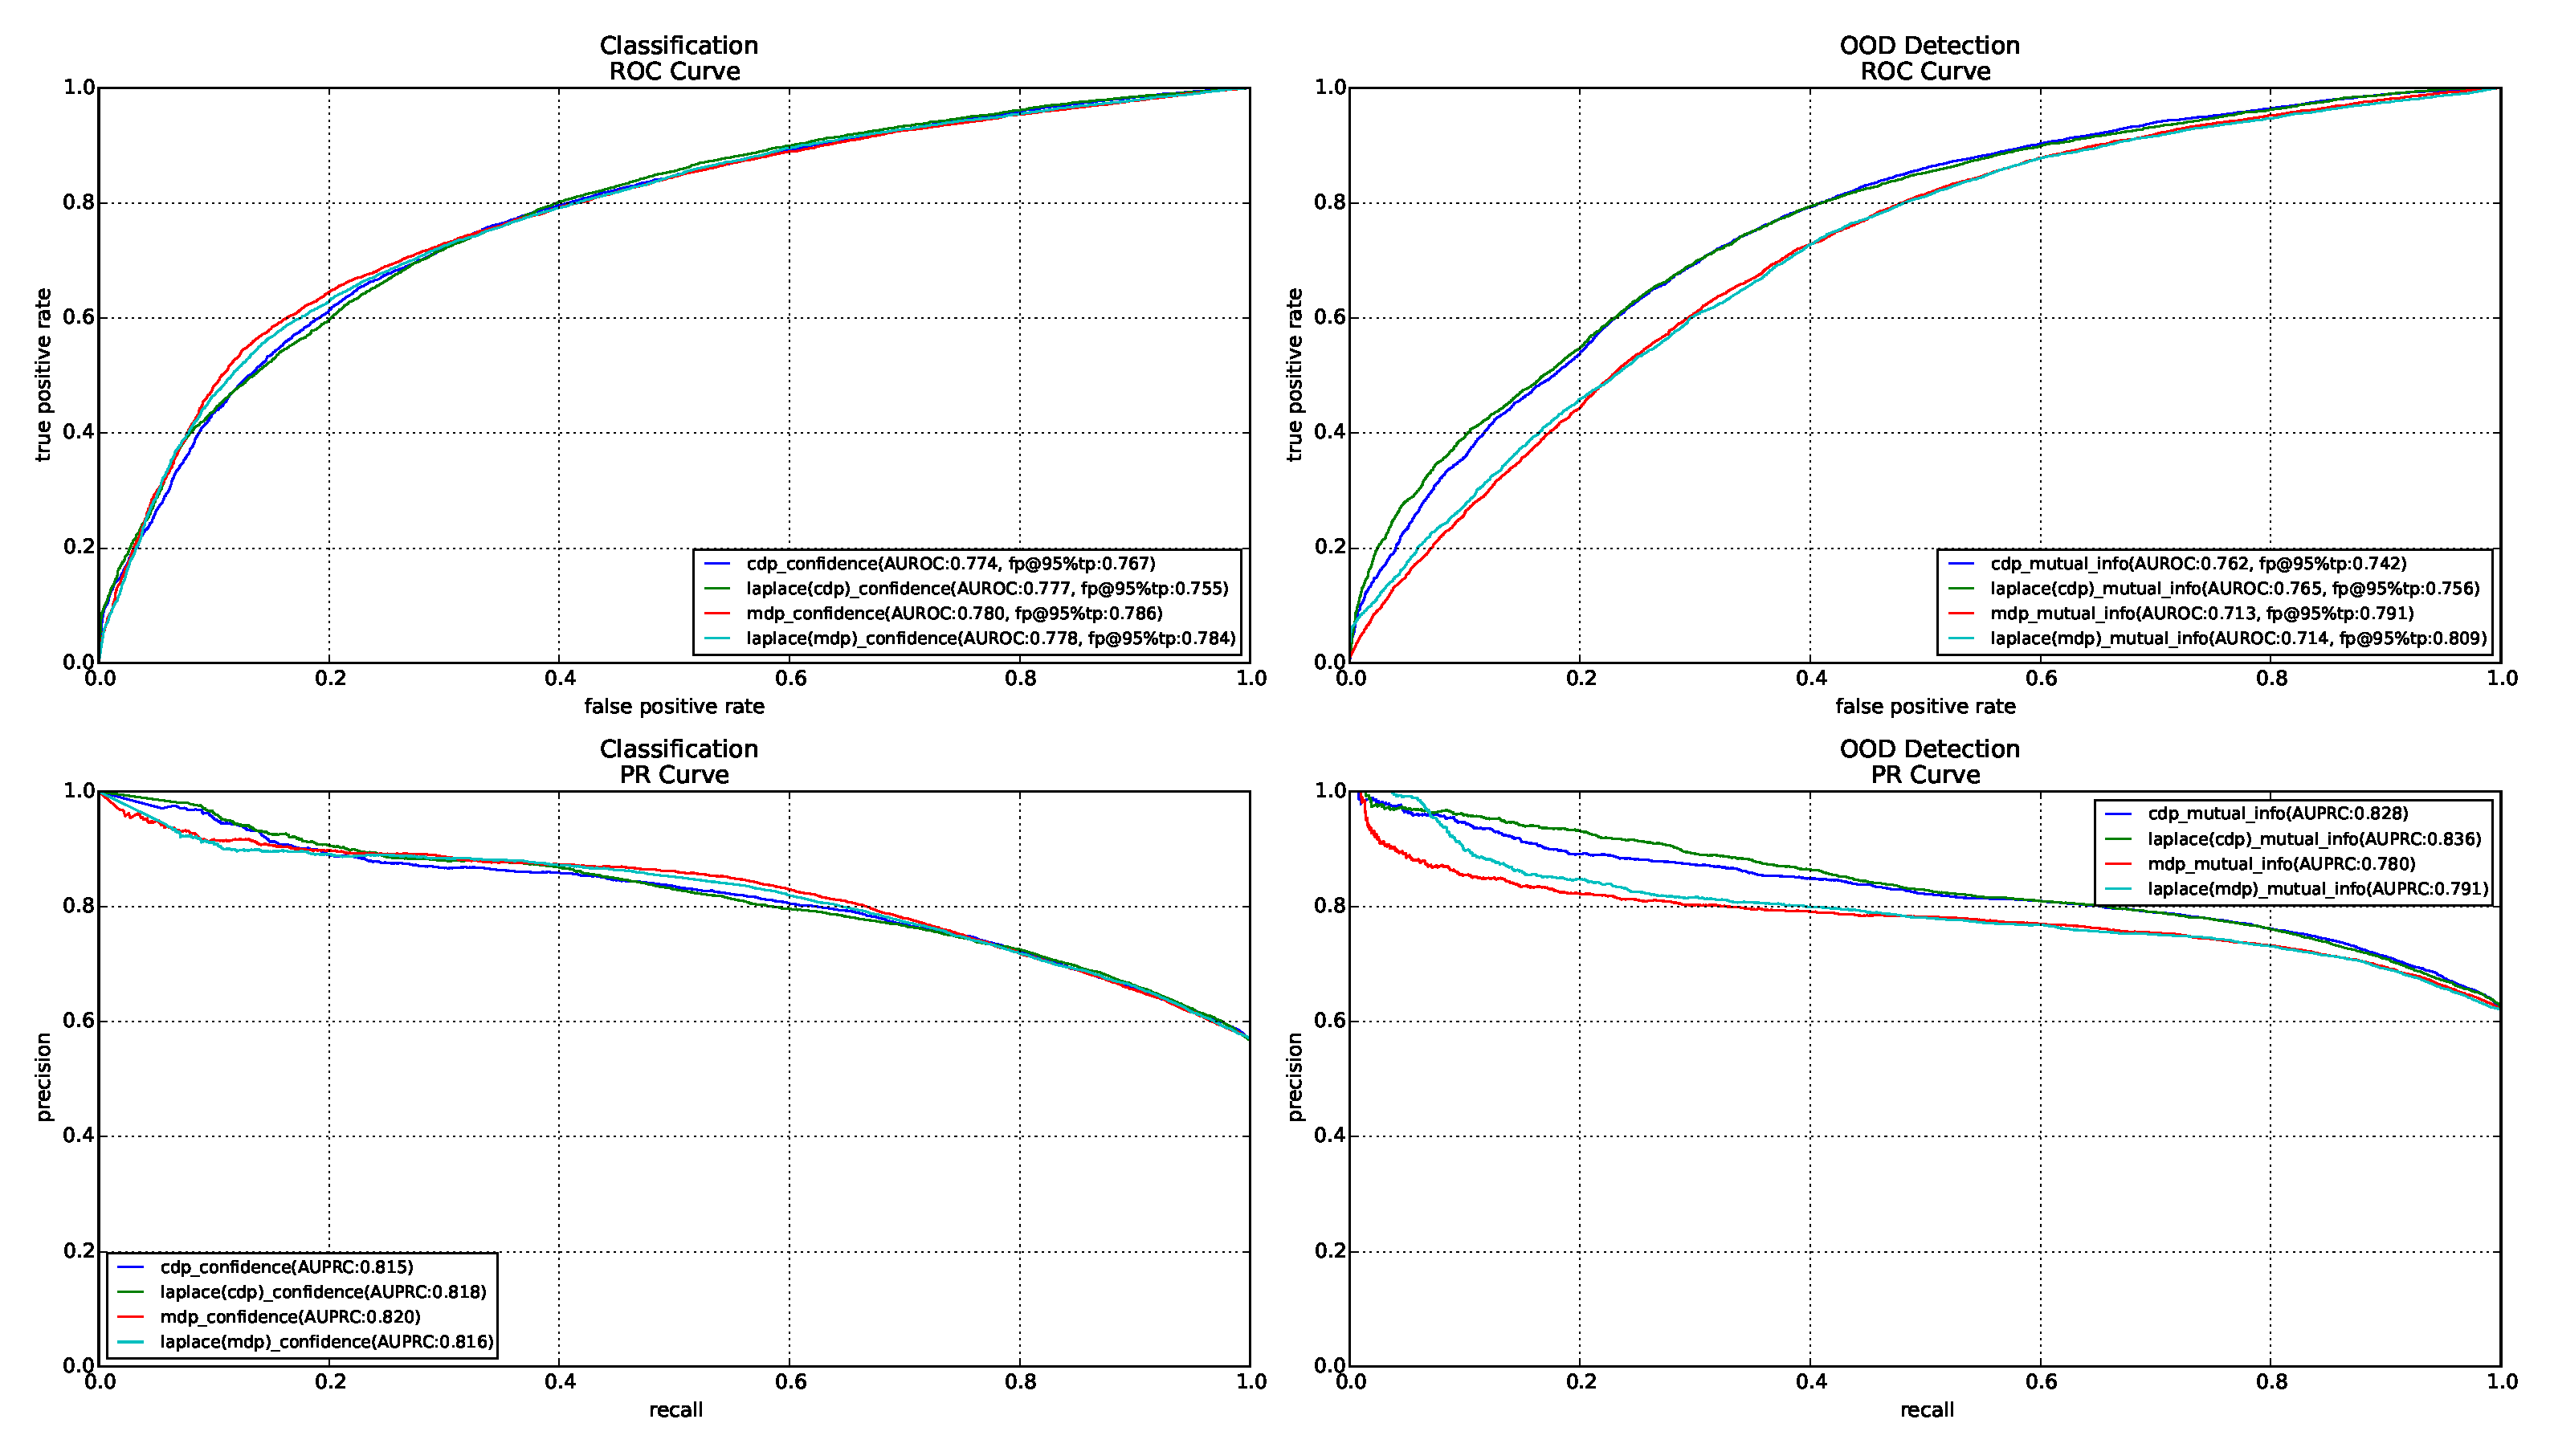
\includegraphics[height=9cm, width=15cm]{uncertainty_estimation/laplace/roc_pr_seed3.eps}
		\caption{ROC and PR curve of cdp, mdp and their Laplace approximation versions in one of three runs.}		
		\label{lap_roc_pr}
	\end{center}
\end{figure}

\begin{table}[H]
	\centering
	\label{table:lap}
	\caption{Quantitative results of acc, bs, nll, ece, mce, auroc, aupr averaged from 3 different random seeds}
	\begin{tabular}{|l|l|l|l|}
		\hline
		& accuracy  $\boldsymbol \uparrow$                                                            & brier score $\boldsymbol \downarrow$                                                           & \begin{tabular}[c]{@{}l@{}}negative \\ log\\ likelihood $\boldsymbol \downarrow$\end{tabular}  \\ \hline
		cdp          & 
		\begin{tabular}[c]{@{}l@{}}0.577$\pm$0.008\end{tabular} & 
		\begin{tabular}[c]{@{}l@{}}0.594$\pm$0.013\end{tabular} & \begin{tabular}[c]{@{}l@{}}2.088$\pm$0.181\end{tabular} \\ \hline
		
		laplace\_cdp & 
		\begin{tabular}[c]{@{}l@{}}0.576$\pm$0.009\end{tabular}    & \begin{tabular}[c]{@{}l@{}}0.602$\pm$0.011\end{tabular} & \begin{tabular}[c]{@{}l@{}}2.322$\pm$0.350\end{tabular} \\ \hline
		
		mdp          & 
		\begin{tabular}[c]{@{}l@{}}\textbf{0.599$\pm$0.023}\end{tabular} & \begin{tabular}[c]{@{}l@{}}\textbf{0.566$\pm$0.020}\end{tabular} & \begin{tabular}[c]{@{}l@{}}\textbf{1.940$\pm$0.064}\end{tabular} \\ \hline
		laplace\_mdp & 		\begin{tabular}[c]{@{}l@{}}0.598$\pm$0.024\end{tabular} & \begin{tabular}[c]{@{}l@{}}0.567$\pm$0.018\end{tabular} & \begin{tabular}[c]{@{}l@{}}1.970$\pm$0.117\end{tabular} \\ \hline
	\end{tabular}
\end{table}
\begin{table}[H]
	\centering
	\begin{tabular}{|l|l|l|l|l|}
		\hline
		& \begin{tabular}[c]{@{}l@{}}expected\\ calibration\\ error(w/o. OOD/\\ w. OOD) $\boldsymbol \downarrow$\end{tabular} & \begin{tabular}[c]{@{}l@{}}maximal\\ calibration\\ error(w/o. OOD/\\ w. OOD)$\boldsymbol \downarrow$\end{tabular} & \begin{tabular}[c]{@{}l@{}}area under\\ ROC\\ (vs. Miss-\\ classified/\\ vs. OOD)$\boldsymbol \uparrow$\end{tabular} & \begin{tabular}[c]{@{}l@{}}area under\\ PR curve\\ (vs. Miss-\\ classified/\\ vs. OOD)$\boldsymbol \uparrow$\end{tabular} \\ \hline
		
		cdp          & \begin{tabular}[c]{@{}l@{}}0.124$\pm$0.023/ \\\textbf{0.288$\pm$0.048}\end{tabular}                      & \begin{tabular}[c]{@{}l@{}}0.206$\pm$0.015/ \\0.374$\pm$0.018\end{tabular}                     & \begin{tabular}[c]{@{}l@{}}0.775$\pm$0.008/ \\\textbf{0.783$\pm$0.022}\end{tabular}           & \begin{tabular}[c]{@{}l@{}}0.825$\pm$0.007/ \\\textbf{0.850$\pm$0.022}\end{tabular}                \\ \hline
		
		laplace\_cdp & \begin{tabular}[c]{@{}l@{}}0.129$\pm$0.058/ \\0.341$\pm$0.157\end{tabular}                         & \begin{tabular}[c]{@{}l@{}}0.235$\pm$0.073/ \\0.406$\pm$0.070\end{tabular}                     & \begin{tabular}[c]{@{}l@{}}0.779$\pm$0.004/ \\0.782$\pm$0.017\end{tabular}           & \begin{tabular}[c]{@{}l@{}}0.826$\pm$0.007/ \\0.849$\pm$0.016\end{tabular}                \\ \hline
		
		mdp          & \begin{tabular}[c]{@{}l@{}}0.114$\pm$0.012/ \\0.383$\pm$0.046\end{tabular}                      & \begin{tabular}[c]{@{}l@{}}0.199$\pm$0.016/ \\0.367$\pm$0.023\end{tabular}                     & \begin{tabular}[c]{@{}l@{}}\textbf{0.780$\pm$0.011}/ \\0.709$\pm$0.004\end{tabular}           & \begin{tabular}[c]{@{}l@{}}\textbf{0.838$\pm$0.013}/ \\0.788$\pm$0.006\end{tabular}                \\ \hline
		
		laplace\_mdp         & \begin{tabular}[c]{@{}l@{}} \textbf{0.104$\pm$0.018}/ \\0.352$\pm$0.061\end{tabular}                      & \begin{tabular}[c]{@{}l@{}}\textbf{0.179$\pm$0.029}/ \\\textbf{0.352$\pm$0.038}\end{tabular}                     & \begin{tabular}[c]{@{}l@{}}0.776$\pm$0.012/ \\0.711$\pm$0.005\end{tabular}           & \begin{tabular}[c]{@{}l@{}}0.837$\pm$0.015/ \\0.798$\pm$0.005\end{tabular}                \\ \hline
	\end{tabular}
\end{table}
\subsubsection{Ablation study}
As we can see from the previous results, mdp can work better than cdp without considering OOD data. However, it underperforms when OOD data is included. In order to investigate the reason behind this, we have done a ablation study to check the influence of aleatoric uncertainty which comes from mainly the feature extractor part. To this end, we firstly make assumption that the feature extractor part has a dominant effect on the aleatoric uncertainty, because it's deterministic compared with the following MLP classifier. 

Considering this, we freeze the parameters of feature extractor trying to keep the dominant effect on aleatoric uncertainty fixed for different approaches and just train our probabilistic classifier which is a three-layer MLP. In the following we show the results of this ablation study with the same metrics used before. It's clear that the accuracy would drop when the feature extractor is frozen. However, we can see that mdp can have better  calibration performance than cdp and much better than original ResNet50. Regarding the separability metrics, although mdp still doesn't work better than cdp, the gap between is much smaller than the version without freezing feature extractor. These observations are expressed quantitatively in the table \ref{ab_table}. 

Based on these observations, we know that the underperformance of mdp on OOD dataset can attribute to the influence of aleatoric uncertainty. If the feature extractor is not frozen, then the aleatoric uncertainty is trained to adapt to the dataset. The problem why optimizing dropout rates for each hidden units can change the point estimate of the model parameter to have low aleatoric uncertainty for OOD data arises here. One possible reason for this could be the variance of estimation of derivatives of variational parameters is too large because of increased number of variational parameters\cite{kingma2015variational}. And the larger variances are back propagated to the feature extractor which may make the point estimate deviate from the better local minimum. One possible solution to resolve this is to sample the realization of activations of hidden units independent to each data instance, which may decrease the variance and help to improve the results. 

\begin{figure}[H]
	\begin{center}
		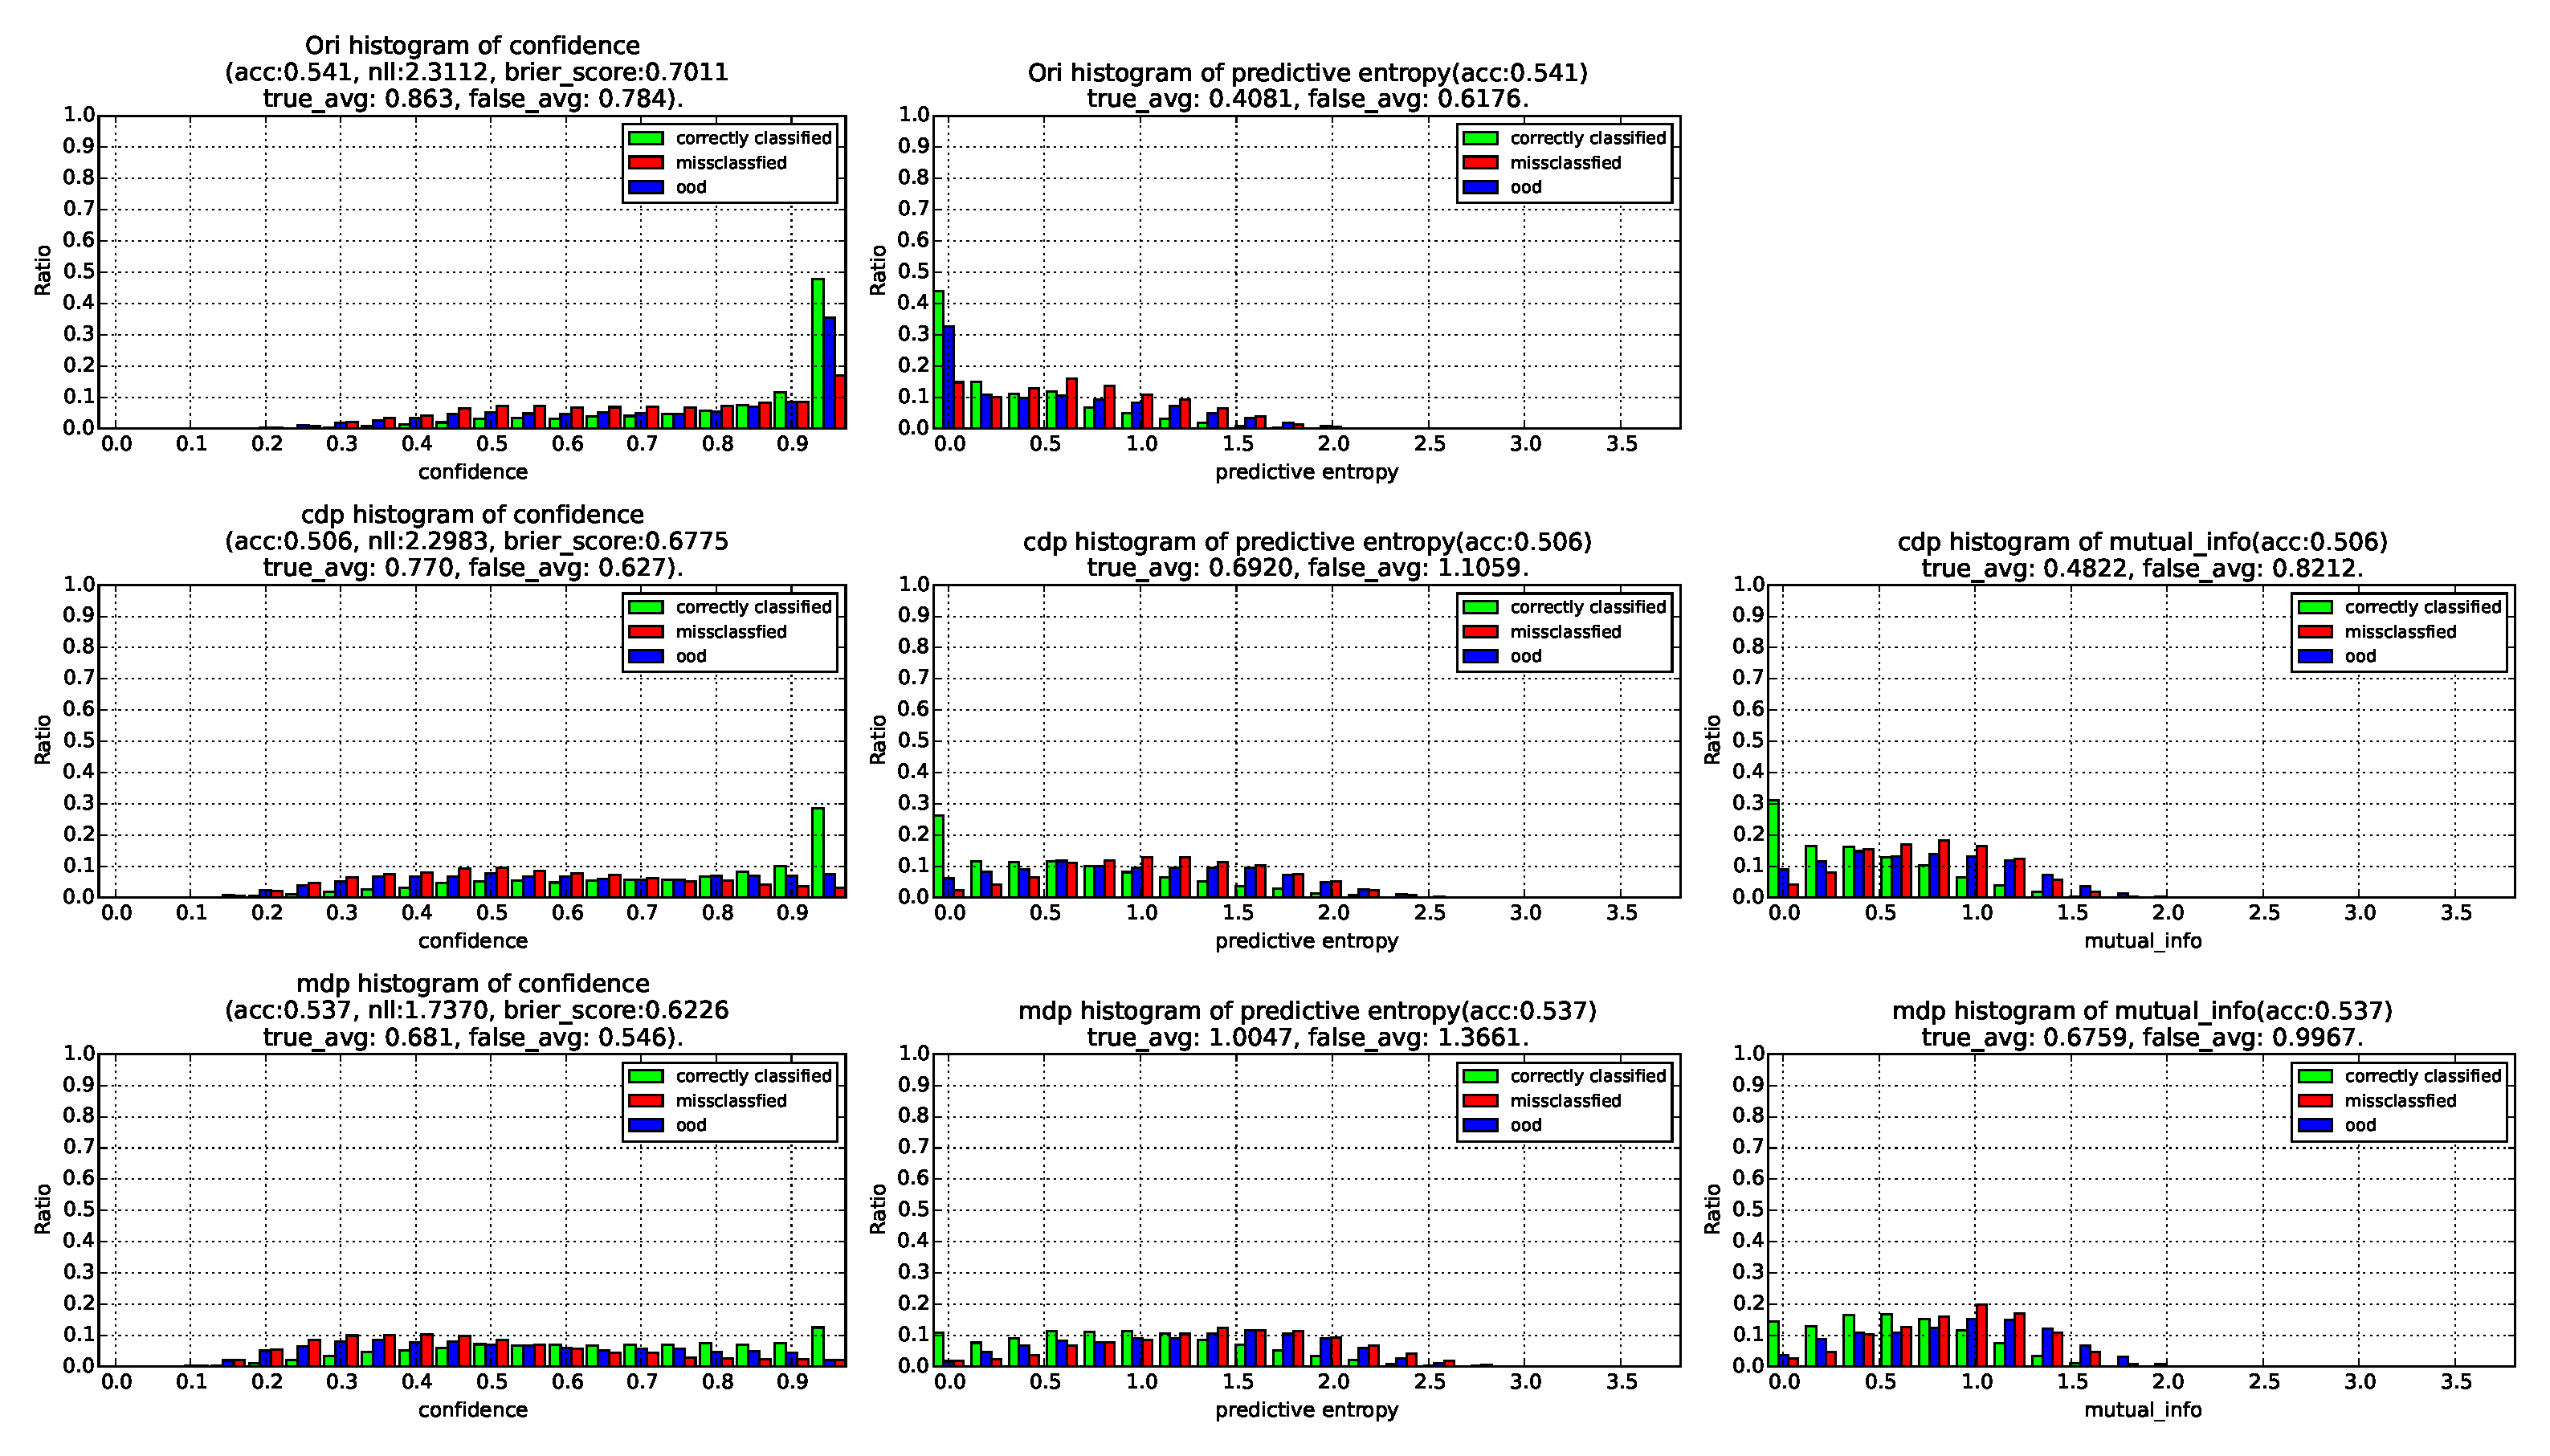
\includegraphics[height=8cm,width=15cm]{uncertainty_estimation/ablation_study/histo_froFeat_ori_cdp_mdp_ood_seed3.eps}
		\caption{Uncertainty histograms of ori, cdp, mdp trained with frozen features in one of three runs.}		
		\label{ab_reliability}
	\end{center}
\end{figure}

\begin{figure}[H]
	\begin{center}
		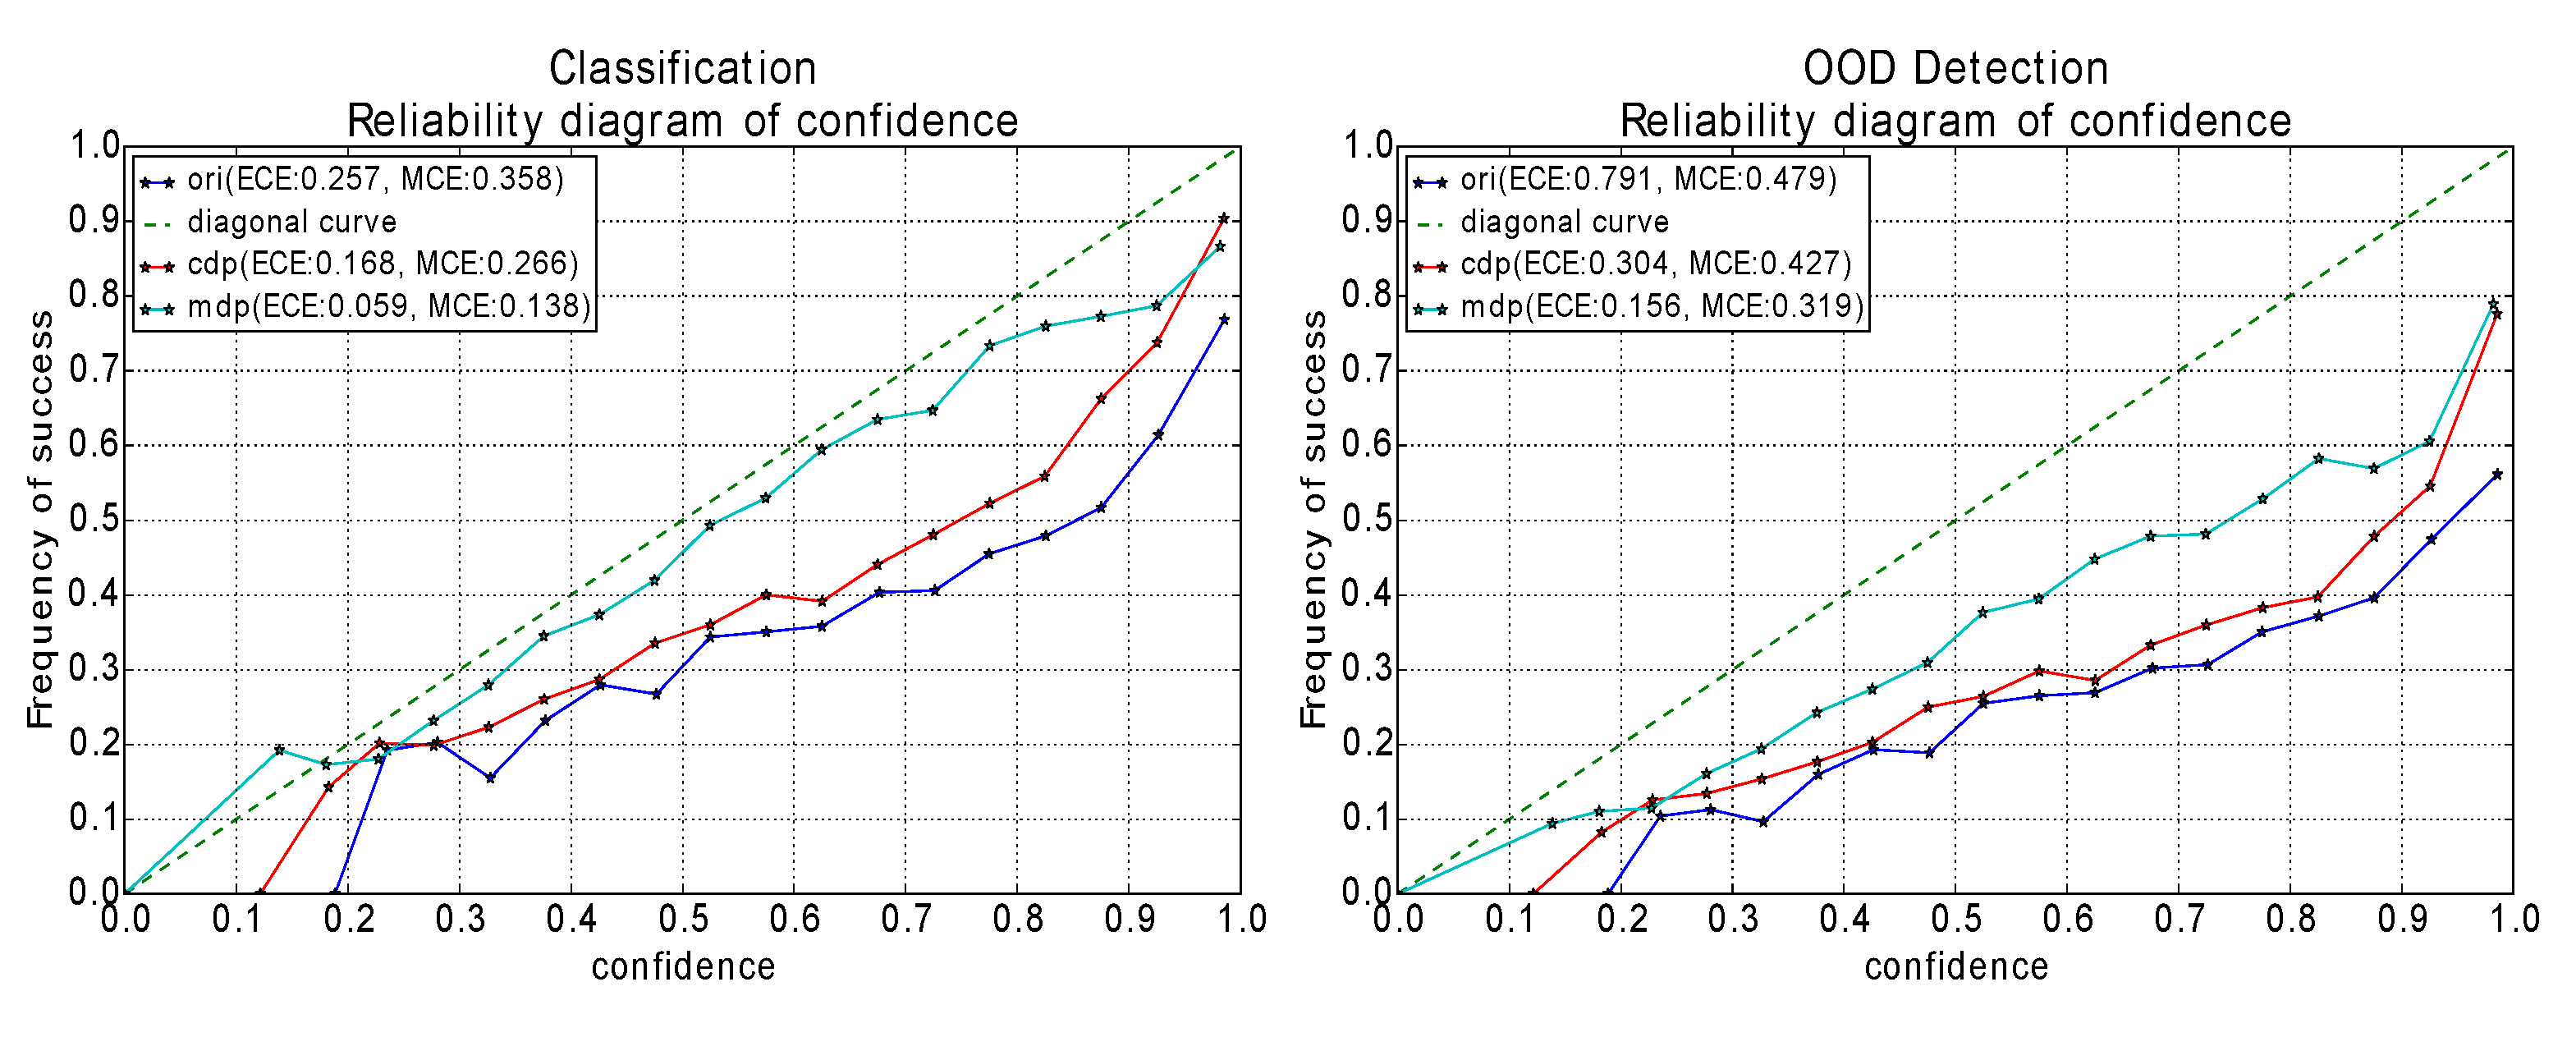
\includegraphics[height=5.5cm, width=15cm]{uncertainty_estimation/ablation_study/reliability_froFeat_ori_cdp_mdp_combined_seed3_.eps}
		\caption{Calibration curves of ori, cdp, mdp trained with frozen features one of three runs.}		
		\label{ab_calibration}
	\end{center}
\end{figure}


\begin{figure}[H]
	\begin{center}
		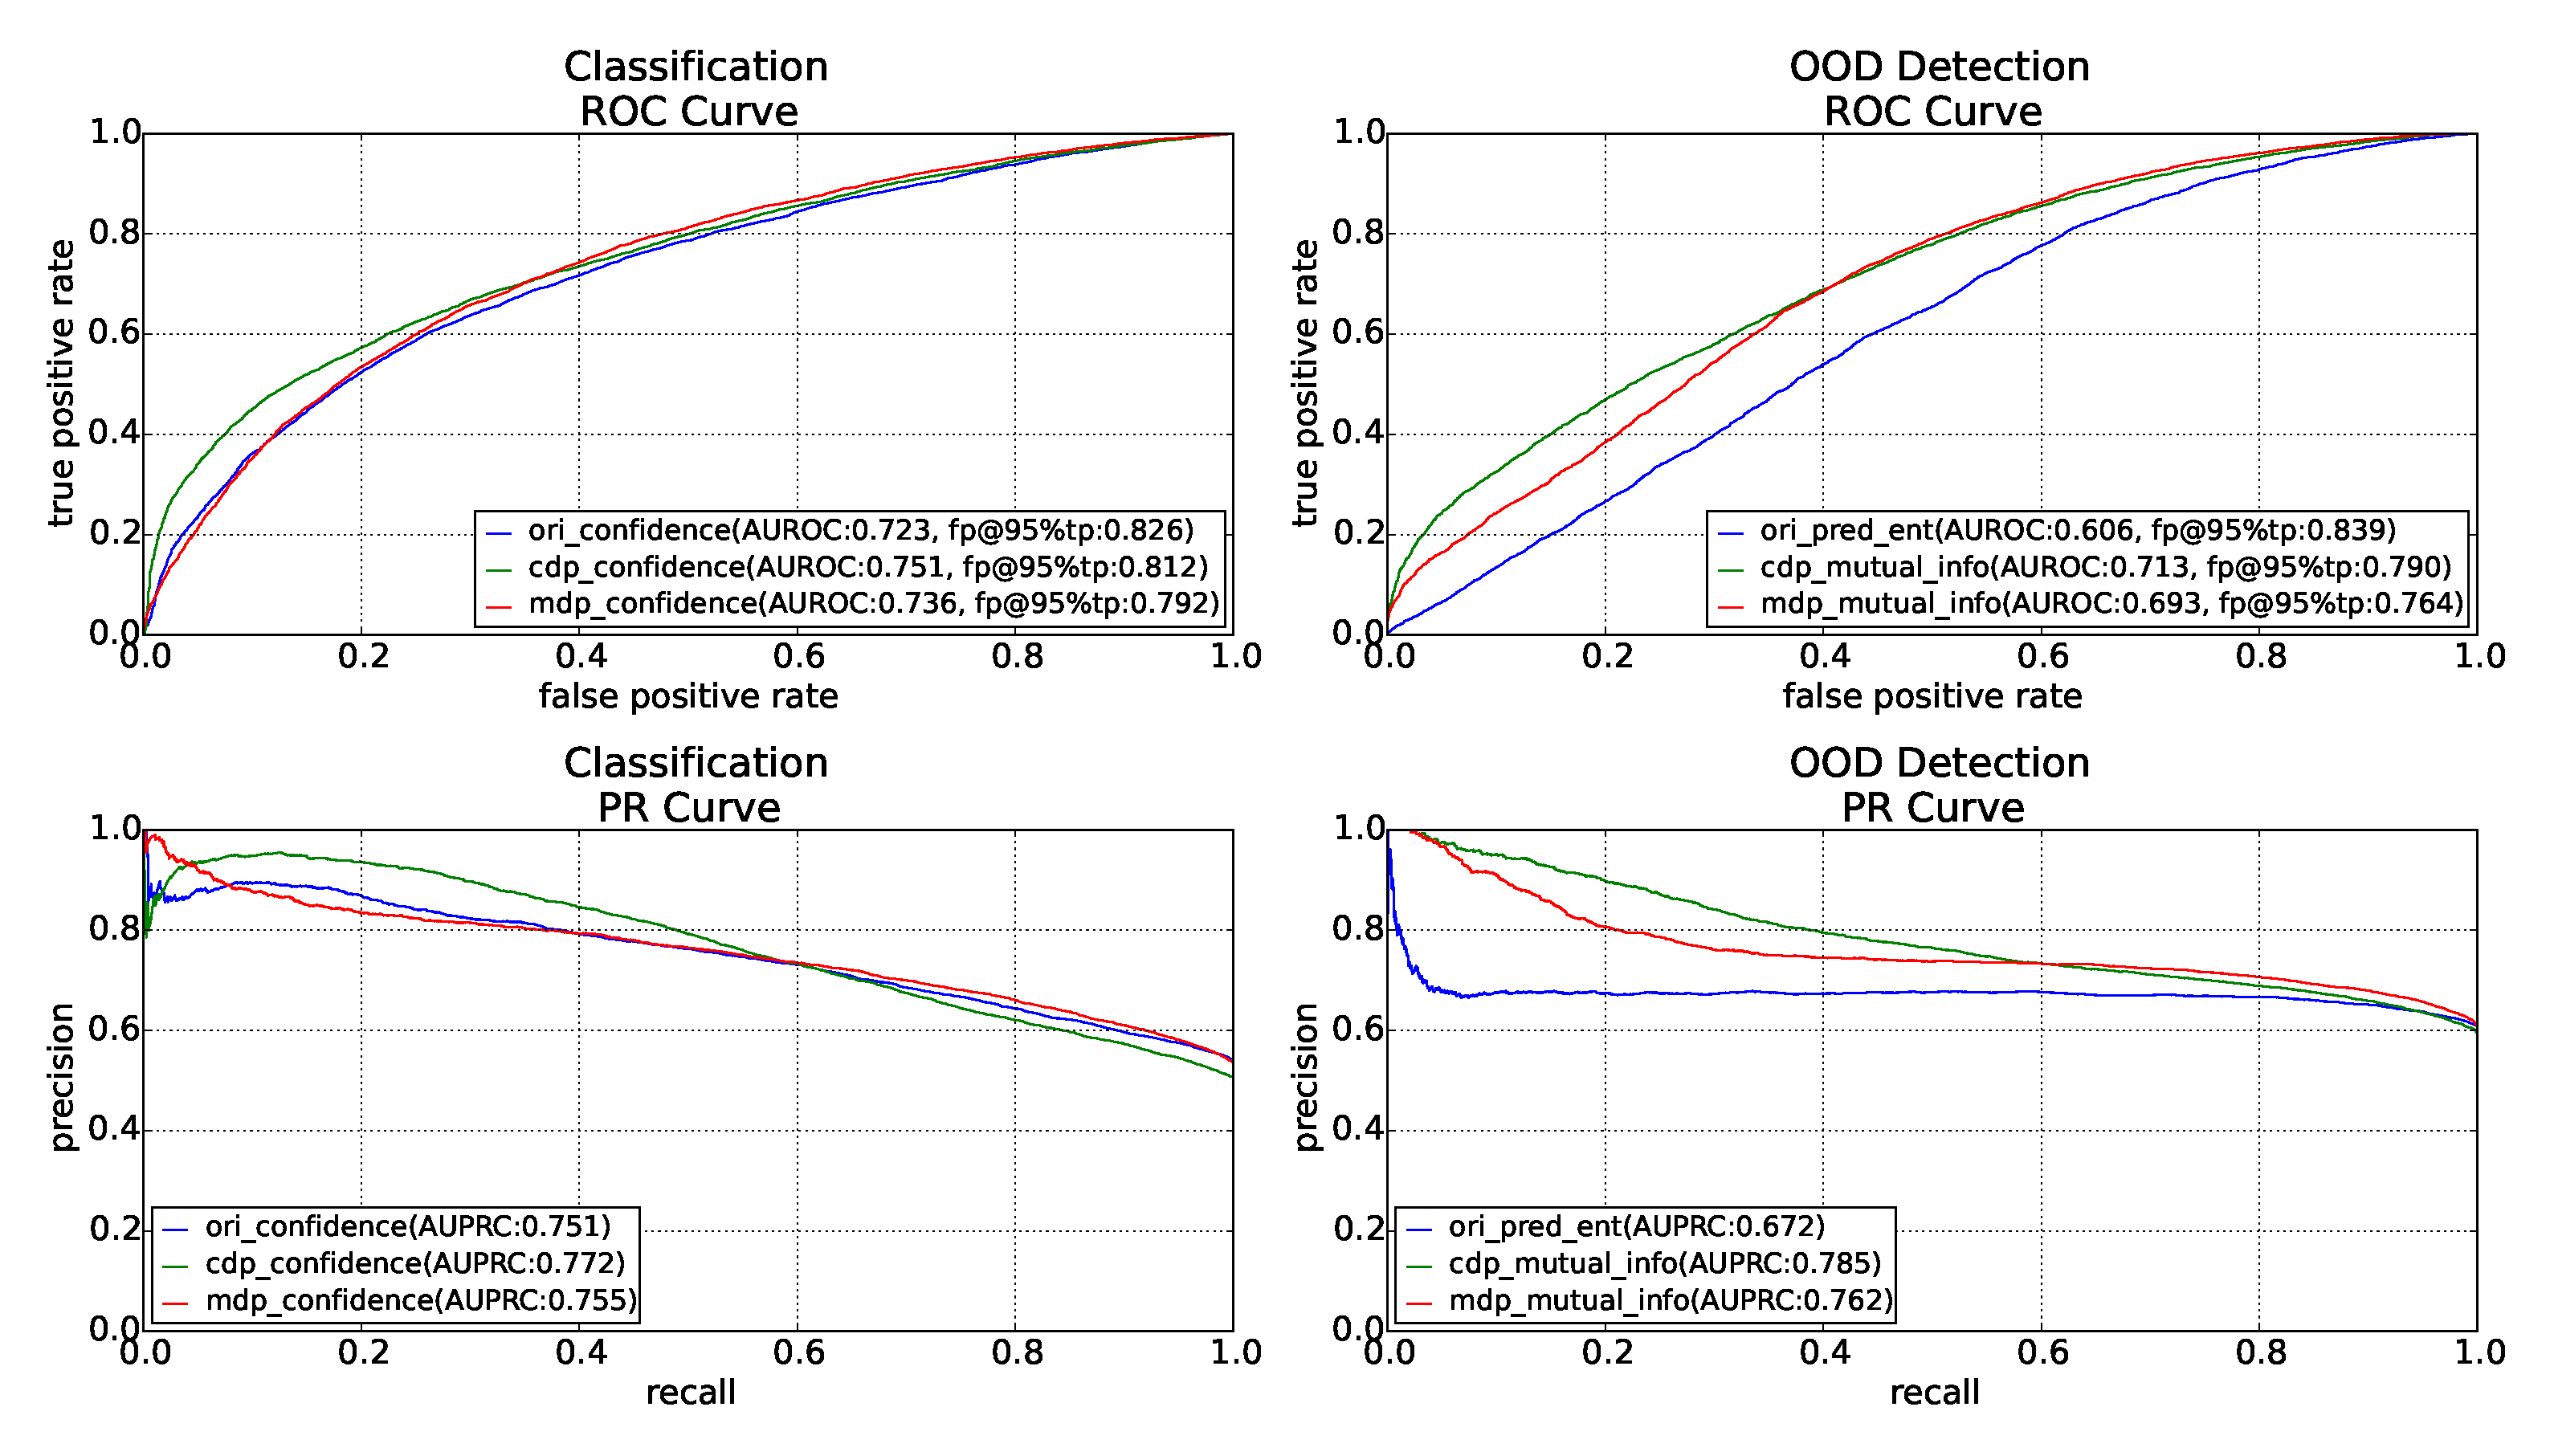
\includegraphics[height=9.5cm, width=15cm]{uncertainty_estimation/ablation_study/roc_pr_froFeat_ori_cdp_mdp_combined_seed3.eps}
		\caption{ROC and PR curves of ori, cdp, mdp trained with frozen features one of three runs.}		
		\label{ab_roc_pr}
	\end{center}
\end{figure}
\begin{table}[H]
	\label{ab_table}
	\centering
	\caption{Quantitative results averaged from 3 random seeds.}
	\begin{tabular}{|l|l|l|l|}
		\hline
		& accuracy   $\boldsymbol \uparrow$  & brier\_score $\boldsymbol \downarrow$& \begin{tabular}[c]{@{}l@{}}negative\\ log \\ likelihood $\boldsymbol \downarrow$\end{tabular} \\ \hline
		ori           &\textbf{0.532$\pm$0.015} & 0.717$\pm$0.023& 2.383$\pm$0.053                                                        \\ \hline
		cdp           & 0.521$\pm$0.011&0.655$\pm$0.017 &  2.190$\pm$0.149                                                        \\ \hline
		mdp           & 0.520$\pm$0.012 &\textbf{0.641$\pm$0.014} & \textbf{1.804$\pm$0.073}                                                         \\ \hline
	\end{tabular}
\end{table}

\begin{table}[H]
	\centering
	% \caption{results of ece, mce, auroc, aupr}
	\begin{tabular}{|l|l|l|l|l|}
		\hline
		& \begin{tabular}[c]{@{}l@{}}expected\\ calibration\\ error(w/o. OOD/\\ w. OOD)$\boldsymbol \downarrow$\end{tabular} & \begin{tabular}[c]{@{}l@{}}maximal\\ calibration\\ error(w/o. OOD/\\ w. OOD)$\boldsymbol \downarrow$\end{tabular} & \begin{tabular}[c]{@{}l@{}}area under\\ ROC\\ (vs. Miss-\\ classified/\\ vs. OOD)$\boldsymbol \uparrow$\end{tabular} & \begin{tabular}[c]{@{}l@{}}area under\\ PR curve\\ (vs. Miss-\\ classified/\\ vs. OOD)$\boldsymbol \uparrow$\end{tabular} \\ \hline
		ori           & \begin{tabular}[c]{@{}l@{}}0.262$\pm$0.011/ \\0.793$\pm$0.012\end{tabular}                      & \begin{tabular}[c]{@{}l@{}}0.365$\pm$0.010/ \\0.491$\pm$0.013\end{tabular}                     &
		\begin{tabular}[c]{@{}l@{}}0.716$\pm$0.005/ \\0.602$\pm$0.014\end{tabular}           & \begin{tabular}[c]{@{}l@{}}0.724$\pm$0.022/ \\0.681$\pm$0.007\end{tabular}                \\ \hline
		cdp           & \begin{tabular}[c]{@{}l@{}}0.141$\pm$0.022/ \\0.270$\pm$0.037\end{tabular}                     & \begin{tabular}[c]{@{}l@{}}0.203$\pm$0.053/ \\0.359$\pm$0.056\end{tabular}                     & \begin{tabular}[c]{@{}l@{}}\textbf{0.748$\pm$0.002}/ \\\textbf{0.712$\pm$0.006}\end{tabular}           & \begin{tabular}[c]{@{}l@{}}\textbf{0.770$\pm$0.002}/ \\\textbf{0.782$\pm$0.004}\end{tabular}                \\ \hline
		
		mdp           & \begin{tabular}[c]{@{}l@{}}\textbf{0.068$\pm$0.009}/ \\\textbf{0.158$\pm$0.006}\end{tabular}                      & \begin{tabular}[c]{@{}l@{}}\textbf{0.134$\pm$0.018}/ \\\textbf{0.311$\pm$0.008}\end{tabular}                     & \begin{tabular}[c]{@{}l@{}}0.730$\pm$0.009/ \\0.674$\pm$0.014\end{tabular}           & \begin{tabular}[c]{@{}l@{}}0.749$\pm$0.009/ \\0.748$\pm$0.010\end{tabular}                \\ \hline
	\end{tabular}
\end{table}	


\section{Automatic labeling experiments}

In experiments of automatic labeling, our goal is to perform a proof-of-concept experiment, which simulates the situation that a classifier trained on a public large scale dataset or synthetic dataset is deployed in a real world environment and tries to fine-tune itself to improve performance with automatically labeled dataset and as little manually labeled data as possible (cf. \ref{fig:con_learn}). The automatically labeled data is collected based on improved uncertainty estimation. Because ResNet50 with concrete dropout shows more stable results than other version, we use it to improve uncertainty estimation in the following experiments and call it \textbf{BNN} without specifications. 

This way to enable the classifier to learn continuously is seldom seen in the literatures. Therefore, in order to investigate the practicability of this method, we firstly perform experiments on WRGBD and UniHB dataset with restriction on the size of collected dataset. 

Then we try to extend this way to another dataset, T-LESS dataset, to test its generalization ability in second experiment. In the second experiment, the situation is similar to the first experiment, where a classifier is firstly trained on synthetic dataset and then deployed in a real world environment which is simulated by the real objects in training set.  We employ data augmentation to address the problem of imbalance in fine-tuning classifier found in the first experiment.
 
\subsection{Experiment \RNum{1}: evaluation on WRGBD and UniHB dataset}
The first experiment is performed on the WRGBD and UniHB dataset. As is mentioned in experiment \RNum{2} of uncertainty estimation experiments, we train BNN with entire WRGBD dataset and evaluate performance of uncertainty estimation on objects of elevation $30^{\circ}$ and $60^{\circ}$ in UniHB dataset, which we call \textbf{adaptation dataset}. The size of adaptation dataset in this experiment is around $\sim$17.1K. The objects of $45^{\circ}$ with size $\sim$8.6K are used for final evaluation after fine-tuning the classifier. The dataset used for fine-tuning are collected from the adaptation set with different settings in order to investigate the issues of this way for continuous learning. 

The uncertainty measure we used is confidence because in this case we do not consider OOD data and confidence performs better in separating correct predictions and miss-classifications based on the results of previous experiments.

\paragraph{Automatic Labeling:}One major restriction we impose in this experiment is the size of dataset for fine-tuning. Because if we do not restrict the size, the performance is influenced by both the size of dataset and other factors such as imbalance or quality of dataset. In order to exclude the influence of dataset size, we fix it as 3\% of the adaptation set which is around 510. If the dataset is balanced in number of data sample of category, then there are around 10 data samples in each category. Then we can investigate how two factors may influence the performance of fine-tuning. 
These two factors are:
\begin{itemize}
	\item the balance in number of data sample of each class 
	\item the amount of information of data samples
\end{itemize}
In the following table \ref{table:fine_tuning}, we describe different settings and use capital letter to denote them.

Here we firstly illustrate the steps of \textbf{selecting automatically labeled data} in this experiment which is a little different to the strategy in experiment \RNum{2}. 

For C, D, E, F, G, we conduct the following steps:
\begin{itemize}
	\item[1.] Automatic labeling: select the most confident predictions and label them with their predictions.
	\item[2.] Manual labeling: select the data randomly or with least confidence required for manual labeling.
	\item[3.] Combining: combine automatically labeled and manually labeled data, then check if any category does not have data sample, if yes add one random data sample of this category.
	\item[4.] Balancing dataset: firstly check if number of data sample of any categories exceed the average number of data sample (which can be calculated beforehand), if yes, drop the data sample of this category randomly until its number reach the average number of category. After that, if augmentation is chosen, then use augmentation to increase of the number of data sample of category in which the number of data sample is less than average number of data sample.

\end{itemize}
To note that, the accuracy of automatically labeled data in C, E, F, G is around 96\%, which means not all labels of them are correct. And "\textbf{randomly}" in this context means that we randomly choose the data of each class with number computed based on the difference between current number of data samples of each class and the average number of data samples of each class. We assume that we have manually labeled all the predictions after automatic labeling and conduct a \textit{proof-of-concept} experiment with \textbf{as balanced as possible} dataset in F and G.    

\begin{table}[H]
	\label{table:fine_tuning}
	\centering
	\caption{Results of fine-tuned network with different settings}
	\begin{tabular}{|l|c|}
		\hline
		Settings of dataset for fine-tuning                                                                                                                                                                                   & \multicolumn{1}{l|}{\begin{tabular}[c]{@{}l@{}}Accuracy\\ (average over 3\\ random seeds)\end{tabular}} \\ \hline
		A: 0\% (no fine-tuning)                                                                                                                                                                                                  & 66.9\%                                                                                                  \\ \hline
		\begin{tabular}[c]{@{}l@{}}B: 3\% manually labeled data randomly \\   (\textbf{balanced})\end{tabular}                                                                                                                               & 91.7\%                                                                                                  \\ \hline
		\begin{tabular}[c]{@{}l@{}}C: 3\% automatically labeled data \\ (\textbf{imbalanced})\end{tabular}                                                                                                                        & 79.0\%                                                                                                  \\ \hline
		\begin{tabular}[c]{@{}l@{}}D: 3\% manually labeled data with least confidence\\ (\textbf{imbalanced})\end{tabular}                                                                                                       & 83.3\%                                                                                                  \\ \hline
		\begin{tabular}[c]{@{}l@{}}E: 2\% automatically labeled data and \\ 1\% manually labeled data with least confidence, \\ augmentation for balance (\textbf{balanced})\end{tabular}                                     & 83.8\%                                                                                                  \\ \hline
		\begin{tabular}[c]{@{}l@{}}F: 2\% automatically labeled data and \\ 0.5\% manually labeled data with least confidence and \\ 0.5\% manually labeled data randomly,\\ augmentation for balance (\textbf{balanced})\end{tabular} & 88.3\%                                                                                                  \\ \hline
		\begin{tabular}[c]{@{}l@{}}G: 2\% automatically labeled data and \\ 1\% manually labeled data randomly,\\ augmentation for balance (\textbf{balanced})\end{tabular}                                                            & 89.6\%                                                                                                  \\ \hline
	\end{tabular}
\end{table}


\paragraph{Fine-tuning:} After collecting the dataset with different settings, we show the results of BNN fine-tuned with those dataset on the final test set which contains only objects of $45^{\circ}$ from UniHB data in the table \ref{table:fine_tuning}. We can draw the following observations from this table:
\begin{itemize}
	\item diverse and balanced dataset can achieved best performance.
	\item the difference of performance between C and D may attribute to quality of dataset which include correct labeling and information of data sample.
	\item by comparing performance of E, F and G, we know that diverse data sample before augmentation is important to achieve better performance. When considering information of data sample, manually labeling of lest confident data sample sounds better. However, we also know that before augmentation dataset in E is more imbalanced than that in F, and F is more imbalanced than G because of the higher proportion of predictions with least confidence. Therefore it shows that data balance is more important than information of data sample in this case.
\end{itemize}
By comparing the results of other settings with that of A and B, we can see that the manual labeling effort can be reduced based on automatic labeling.  The performance of fine-tuned domain specific classifier can nearly reach the the performance of classifier fine-tuned with all manually labeled data. 

In the end, we can draw a conclusion that diversity of data and balance of number of data sample of each category play an significant role. Based on the last aforementioned observation, balance of number of data sample of each category is more important in than information of data sample.

\subsection{Experiment \RNum{2}: evaluation on T-LESS dataset} \label{con_learn_tless}
In this experiment, original ResNet50 and BNN are trained on synthetic dataset introduced in section \ref{tless}. Then automatically labeled data is collected by testing the trained model on real single objects (original training set of T-LESS) which we call \textbf{adaptation dataset}. The difference between the strategy of selecting data in experiment \RNum{1} is that threshold used for selecting data based on uncertainty is chosen on validation set. The accuracy of predictions with uncertainty smaller than this threshold is set as 95\%. Validation set is split off from training set with ratio 2:8. The reason why we use this way to choose threshold is that it's more practical and closer to the real world applications. In this experiment predictive entropy is selected as uncertainty measure, because it shows better performance in term of separability metrics on validation set.

The improved uncertainty estimation from BNN plays an important role here, because it not only provides a reliable uncertainty estimation, but also increases the separability between correct predictions and false predictions, which is more useful in this task. 

\paragraph{Automatic labeling:}
We show the comparisons of uncertainty estimation in term of different evaluation metrics with BNN and original ResNet50 in the following figures. As can be seen in the uncertainty histogram (cf.\ref{autoLa_exp2_hist}), the mode of distribution of uncertainty estimation between correct prediction and miss-classification is further from each other when testing with BNN than with original ResNet50. In Fig.\ref{autoLa_exp2_cali}, BNN expresses better performance in terms of both calibration and separability metrics. 

With the same procedure of selecting automatically labeled data, the size of dataset is around $\sim$1.05K with only 93\% accuracy using original ResNet50, but around $\sim$1.6K with 96\% accuracy using BNN. Because original ResNet50 produces less automatically labeled data with lower quality, the dataset for fine-tuning is collected with BNN.

\begin{figure}[H]
	\begin{center}
		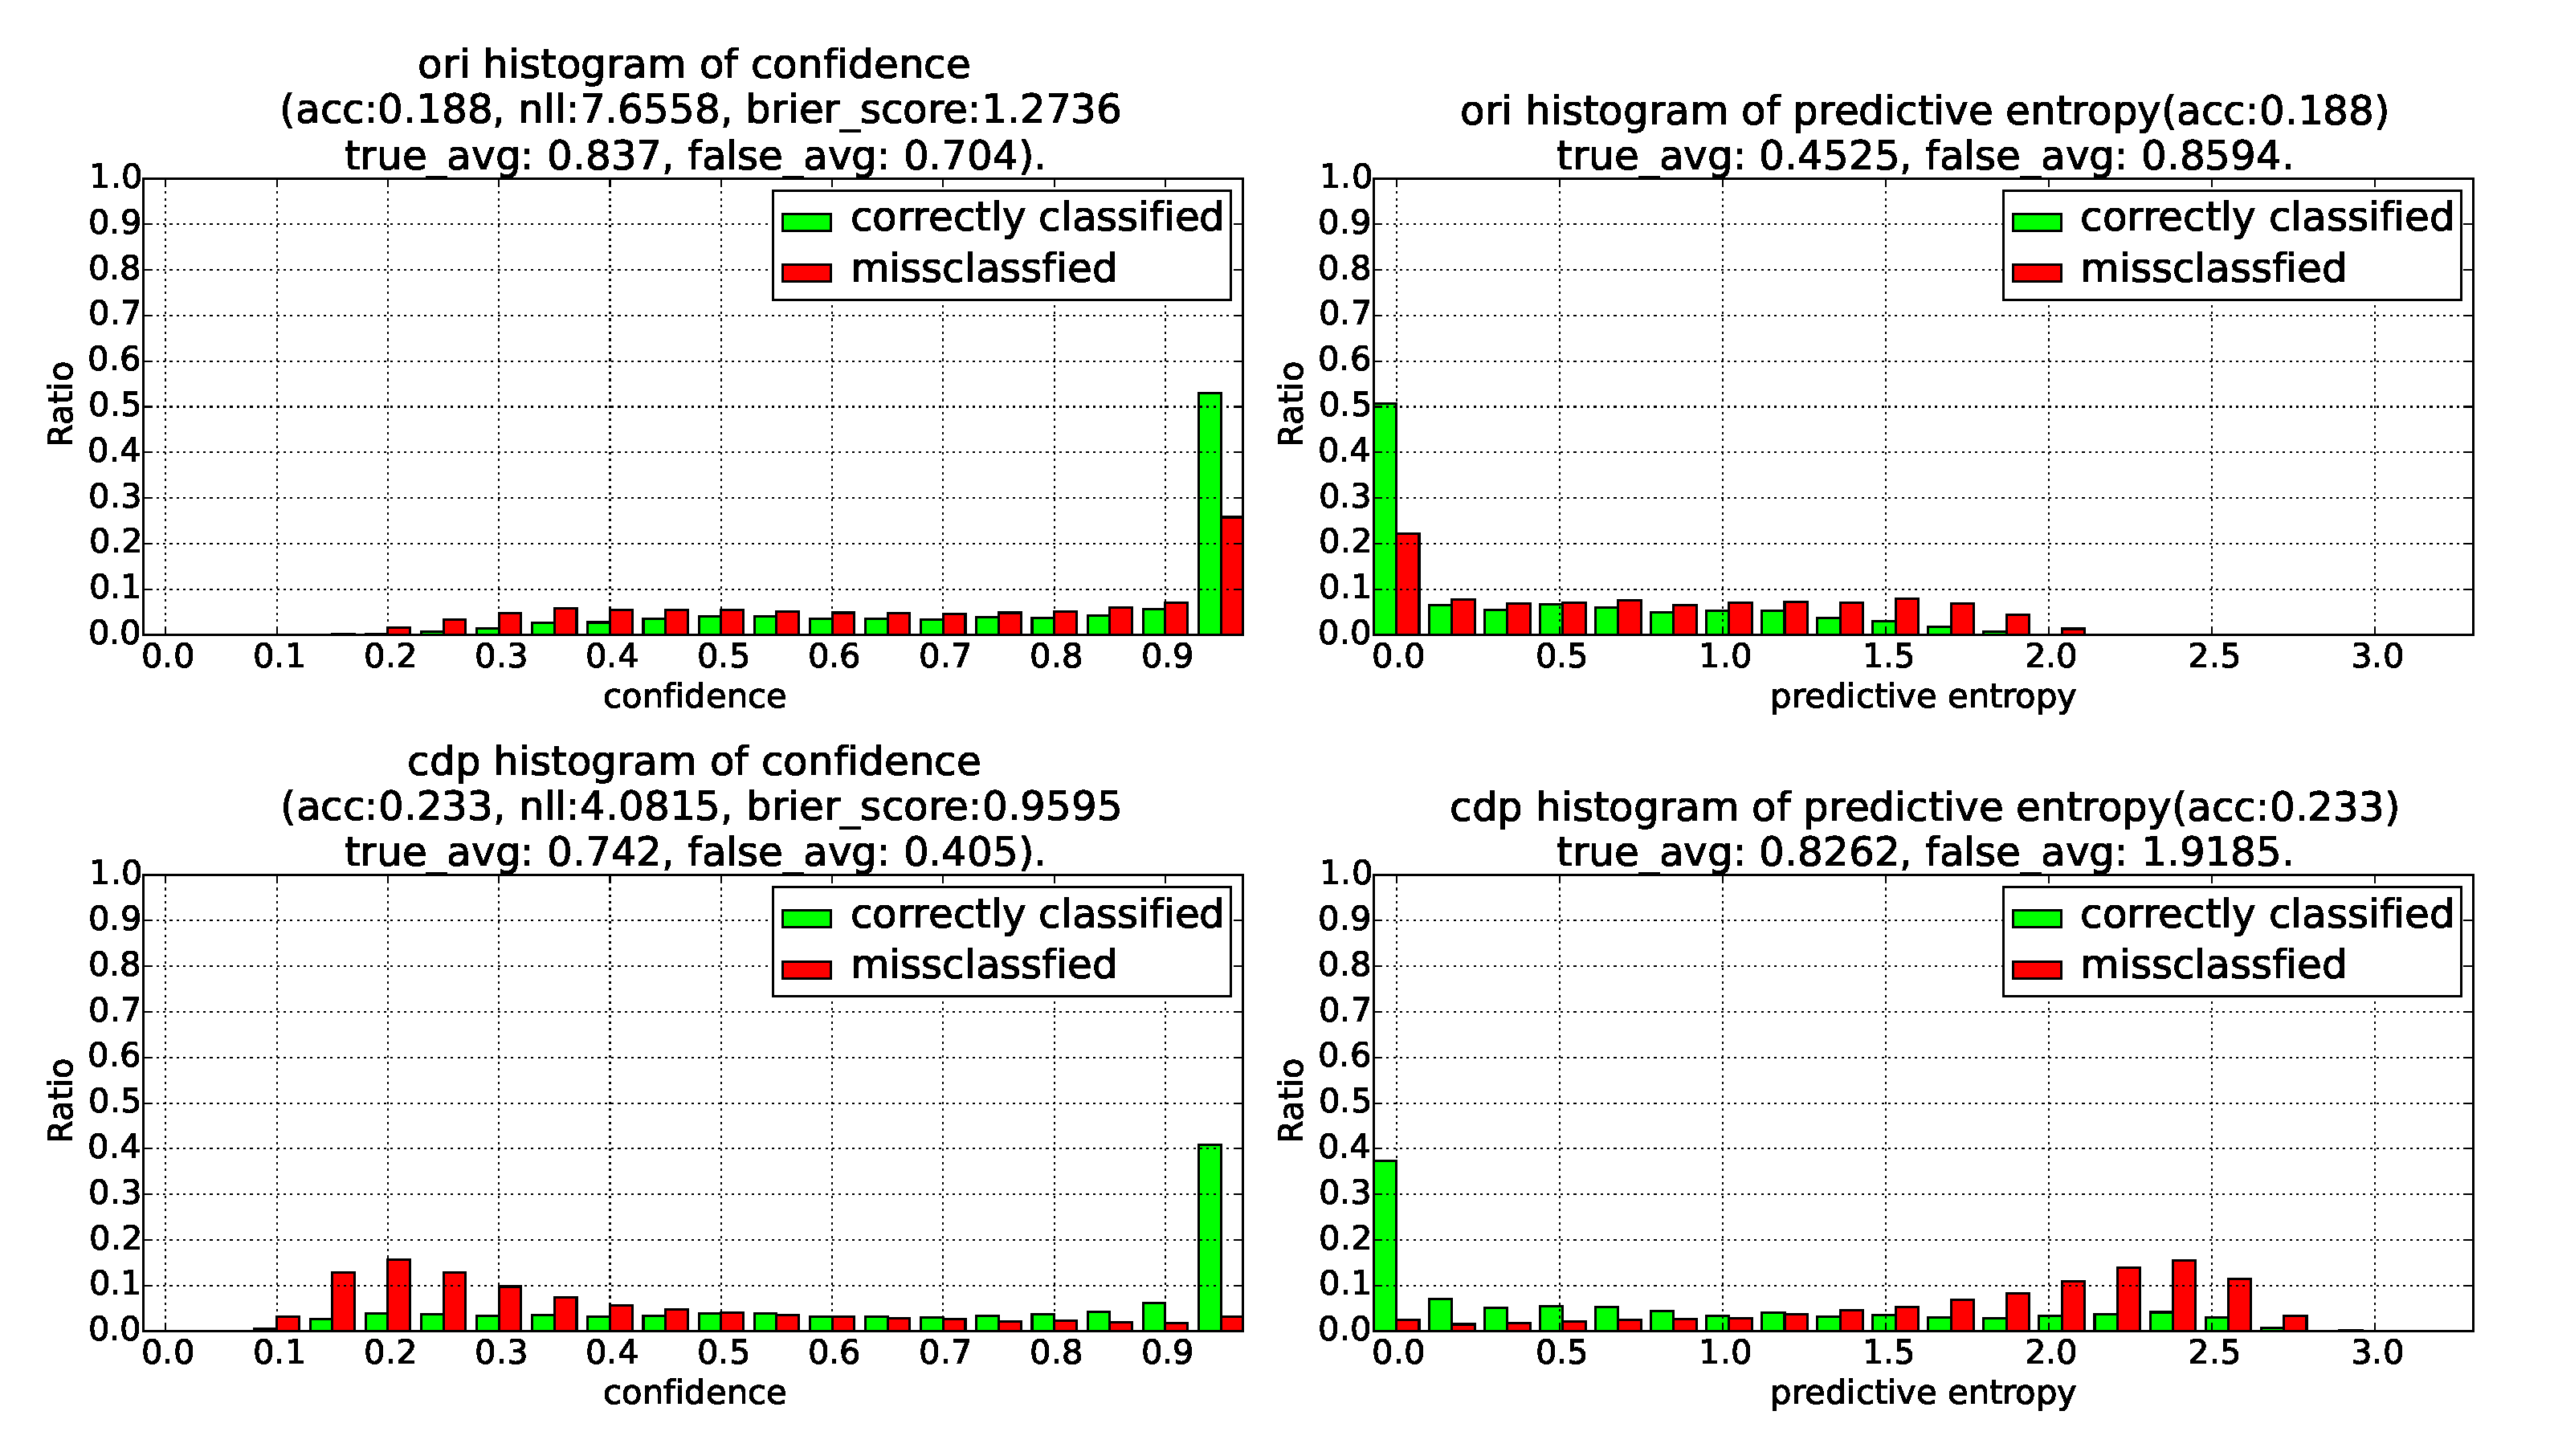
\includegraphics[height=7cm,width=12cm]{autoLa/exp2/syn_cdp_trn_uncer_hist.eps}
		\caption{Uncertainty histograms of original ResNet50 (top) and BNN (down).}		
		\label{autoLa_exp2_hist}
	\end{center}
\end{figure}


However, as found in experiment \RNum{1}, the problem of imbalance in number of data samples of each class still appears on this dataset and has a large influence on the performance. The horizontal histogram in Fig.\ref{hist_class} reveals this problem, in which most of confident predictions cluster in few classes which are class 6, 7, 28 and so on. To mitigate this problem, two simple ways are adopted here:
\begin{itemize}
\item to manually label data uniformly with size 3\% of the adaptation set(around $\sim$0.9K data samples).
\item to employ augmentations described in section \ref{tless} to the objects to balance the dataset as much as possible.  
\end{itemize} 
The balance of dataset with/without manually labeled data after augmentations are showed in Fig.\ref{hist_class}. By using augmentations, datasets are more balanced than before. But the balance before augmentations has significant effect on the performance, which is discussed in the following.

\begin{figure}[H]
	\begin{center}
		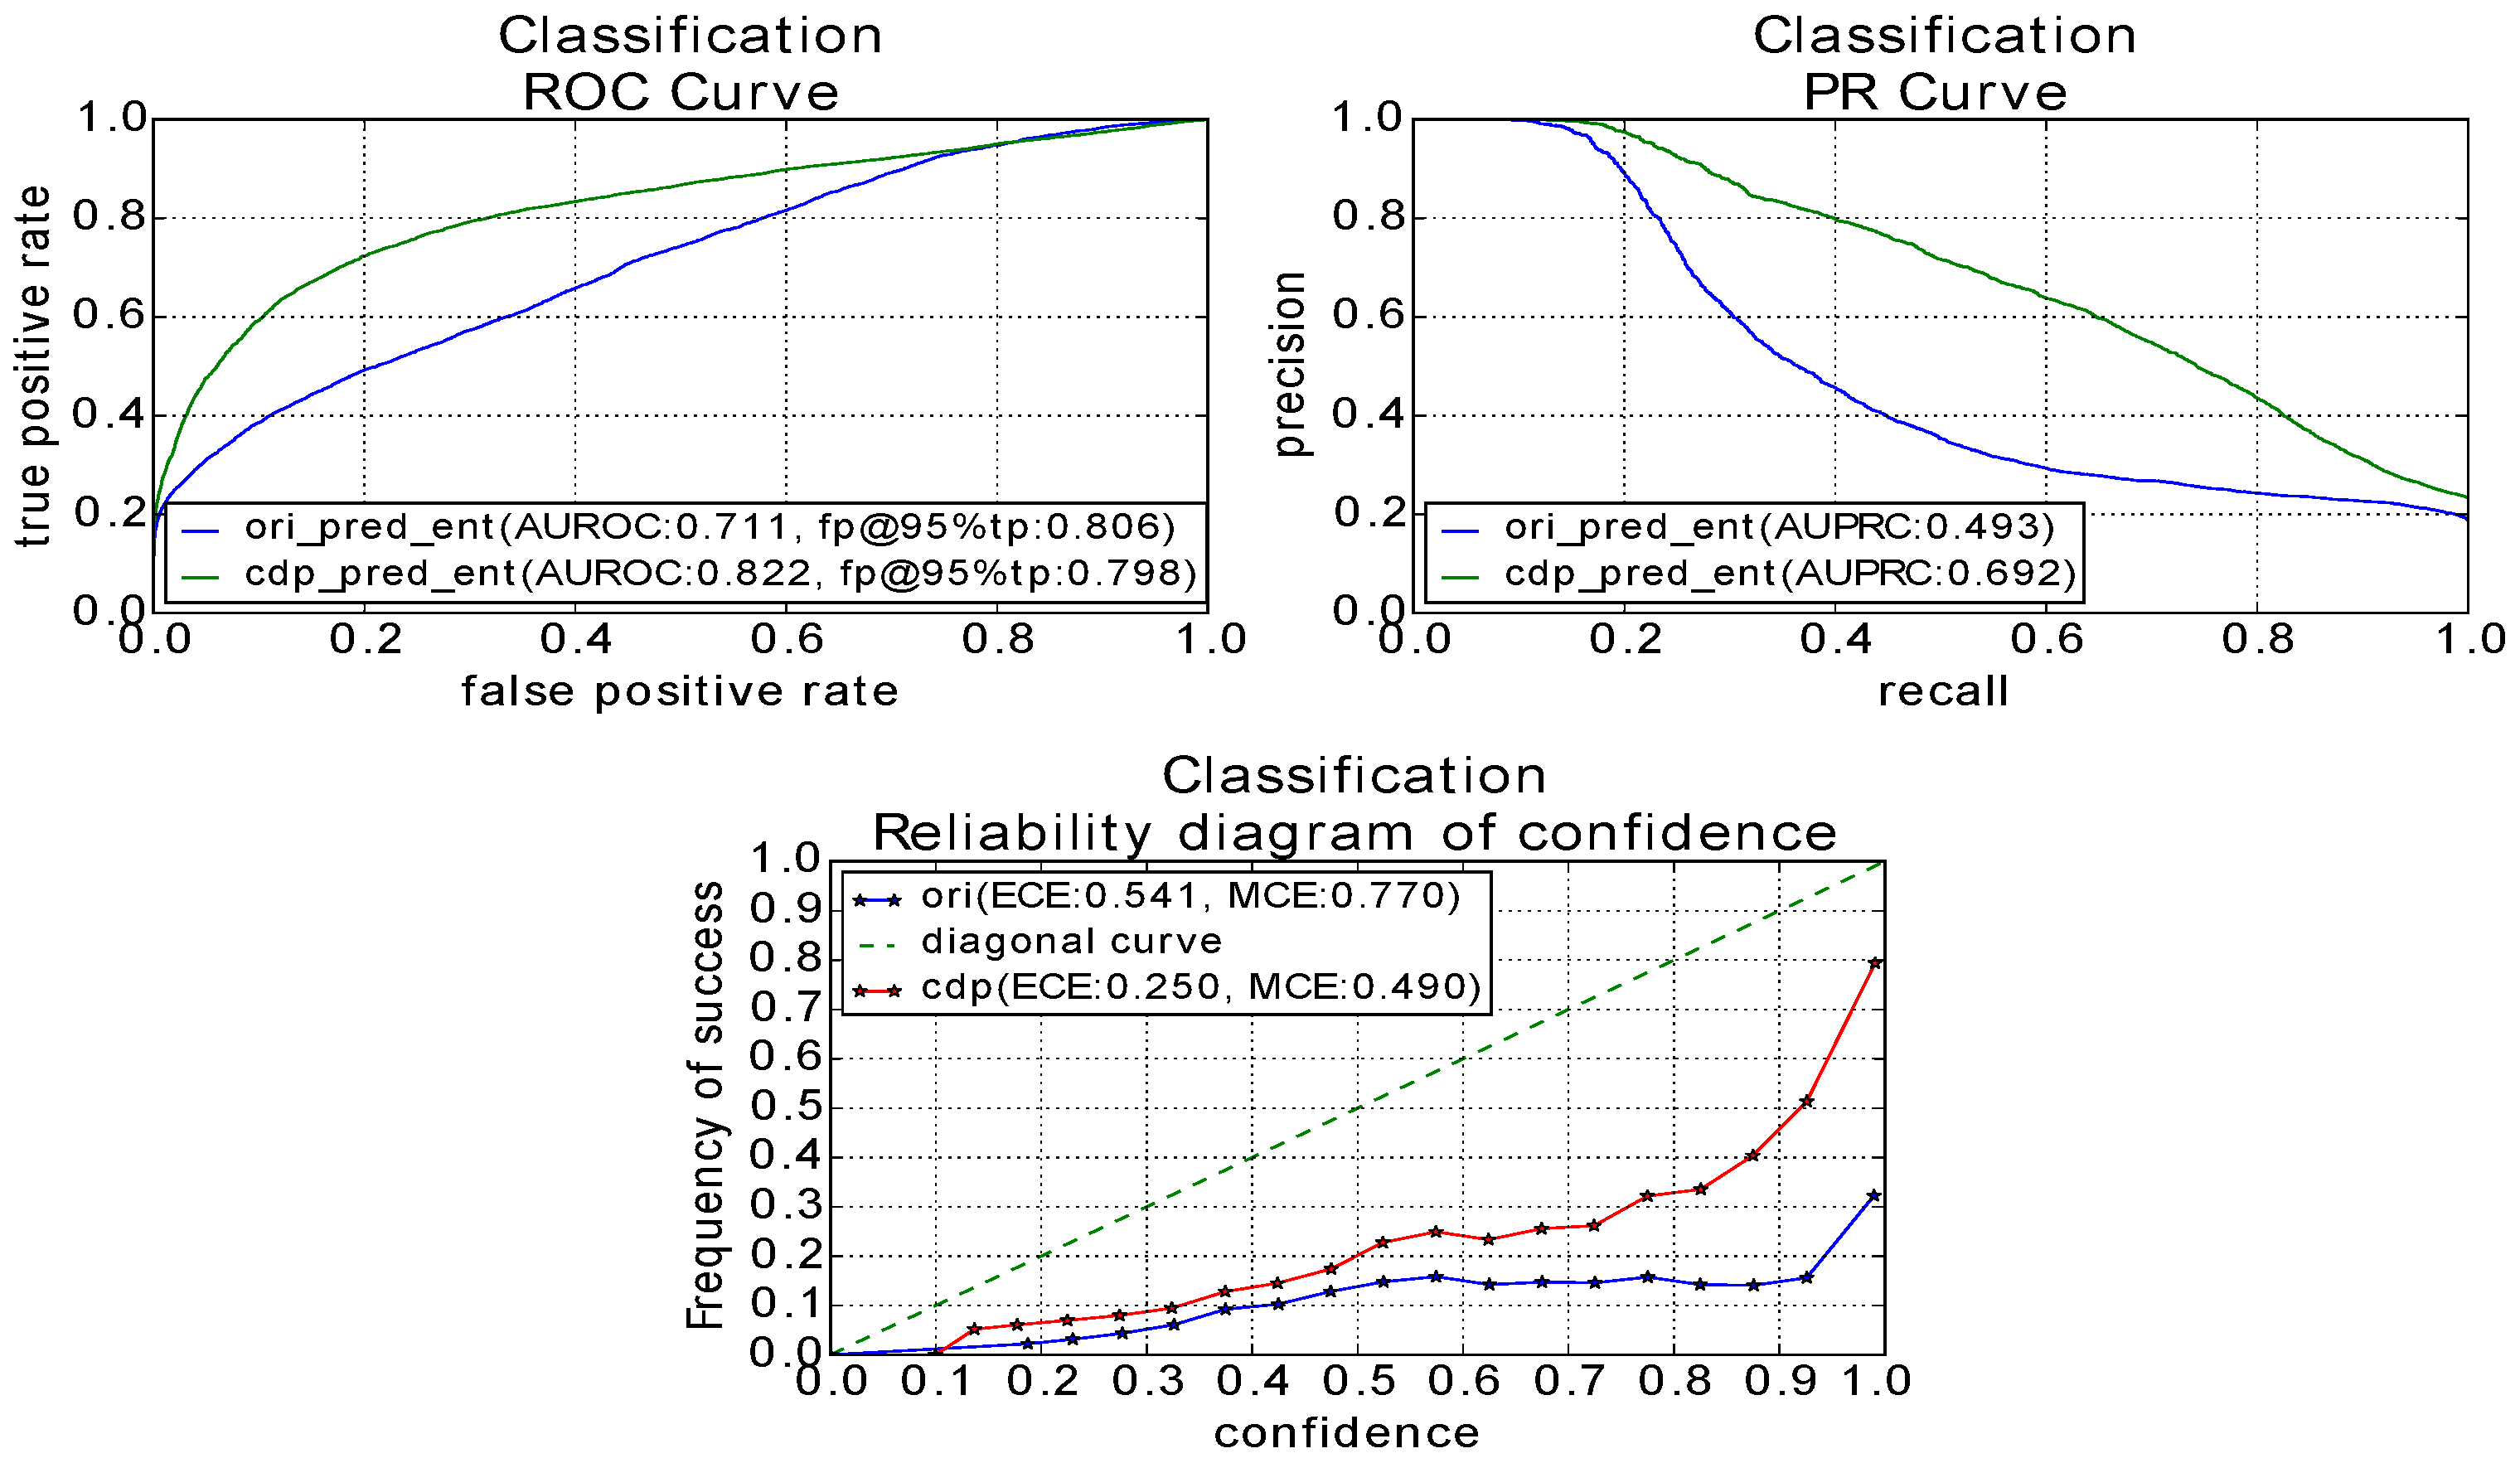
\includegraphics[height=9cm,width=13.5cm]{autoLa/exp2/syn_cdp_trn_roc_pr_cali_.eps}
		\caption{Calibration curves, ROC curves, PR curves of original ResNet50 and BNN.}		
		\label{autoLa_exp2_cali}
	\end{center}
\end{figure}

%\begin{figure}[H]
%	\centering
%	\begin{center}
%		\includegraphics[height=7cm,width=13cm]{autoLa/exp2/syn_cdp_trn_cmf.eps}
%		\caption{Confusion matrix of automatically labeled dataset(label index starts from 0).}		
%		\label{autoLa_exp2_cfm}
%	\end{center}
%\end{figure}

\paragraph{Fine-tuning:} BNNs trained with only synthetic data previously are fine-tuned on dataset collected with different strategies. Table \ref{fine_tune_table} gives the results of BNN trained with different dataset. They are all tested on the test set of T-LESS dataset. By comparing A and B, the performance drop caused by the domain gap between synthetic objects and real ones is quite large, around 35\%. By fine-tuning model on dataset collected based on uncertainty estimation, the accuracy increases a lot. With more balanced dataset, the accuracy even exceed the model trained with augmented entire real dataset by around 3\%. By comparing C and D, it's obvious that the balance of data samples in each class before augmentation is important to obtain more accuracy gain. The reason behind that is the diversity of data samples before augmentation. Although augmentation can help the model generalize better by increasing the number of data samples, if the distribution of training set is poorly represented by few training samples, the way does not help much. This can also be observed in comparison of the corresponding confusion matrices in Fig.\ref{cfm_fine_tune_bnn}, even though the number of data samples in some classes are similar after augmentation, their accuracies differ a lot (35\% vs. 65\% in class 0).

\begin{table}[H]
	\centering
	\label{fine_tune_table}
	\caption{Results of BNN trained with different dataset (size of dataset before augmentations is showed in the bracket).}
	\begin{tabular}{|l|c|}
		\hline
		Setting of dataset                                                                                                                                    & \multicolumn{1}{l|}{Accuracy} \\ \hline
		A: augmented, synthetic dataset                                                                                                                       & 34.91\%                       \\ \hline
		B: augmented, entire real dataset ($\sim$30K)                                                                                                         & 69.58\%                       \\ \hline
		\begin{tabular}[c]{@{}l@{}}C: fine-tune A with \\ augmented, only automatically \\ labeled real dataset ($\sim$1.6K)\end{tabular}                     & 44.99\%                       \\ \hline
		\begin{tabular}[c]{@{}l@{}}D: fine-tune A with \\ augmented, automatically labeled \\ and 3\% manually labeled real dataset ($\sim$2.5K)\end{tabular} & 72.48\%                       \\ \hline
	\end{tabular}
\end{table}


\begin{figure}[H]
	\centering
	\begin{center}
		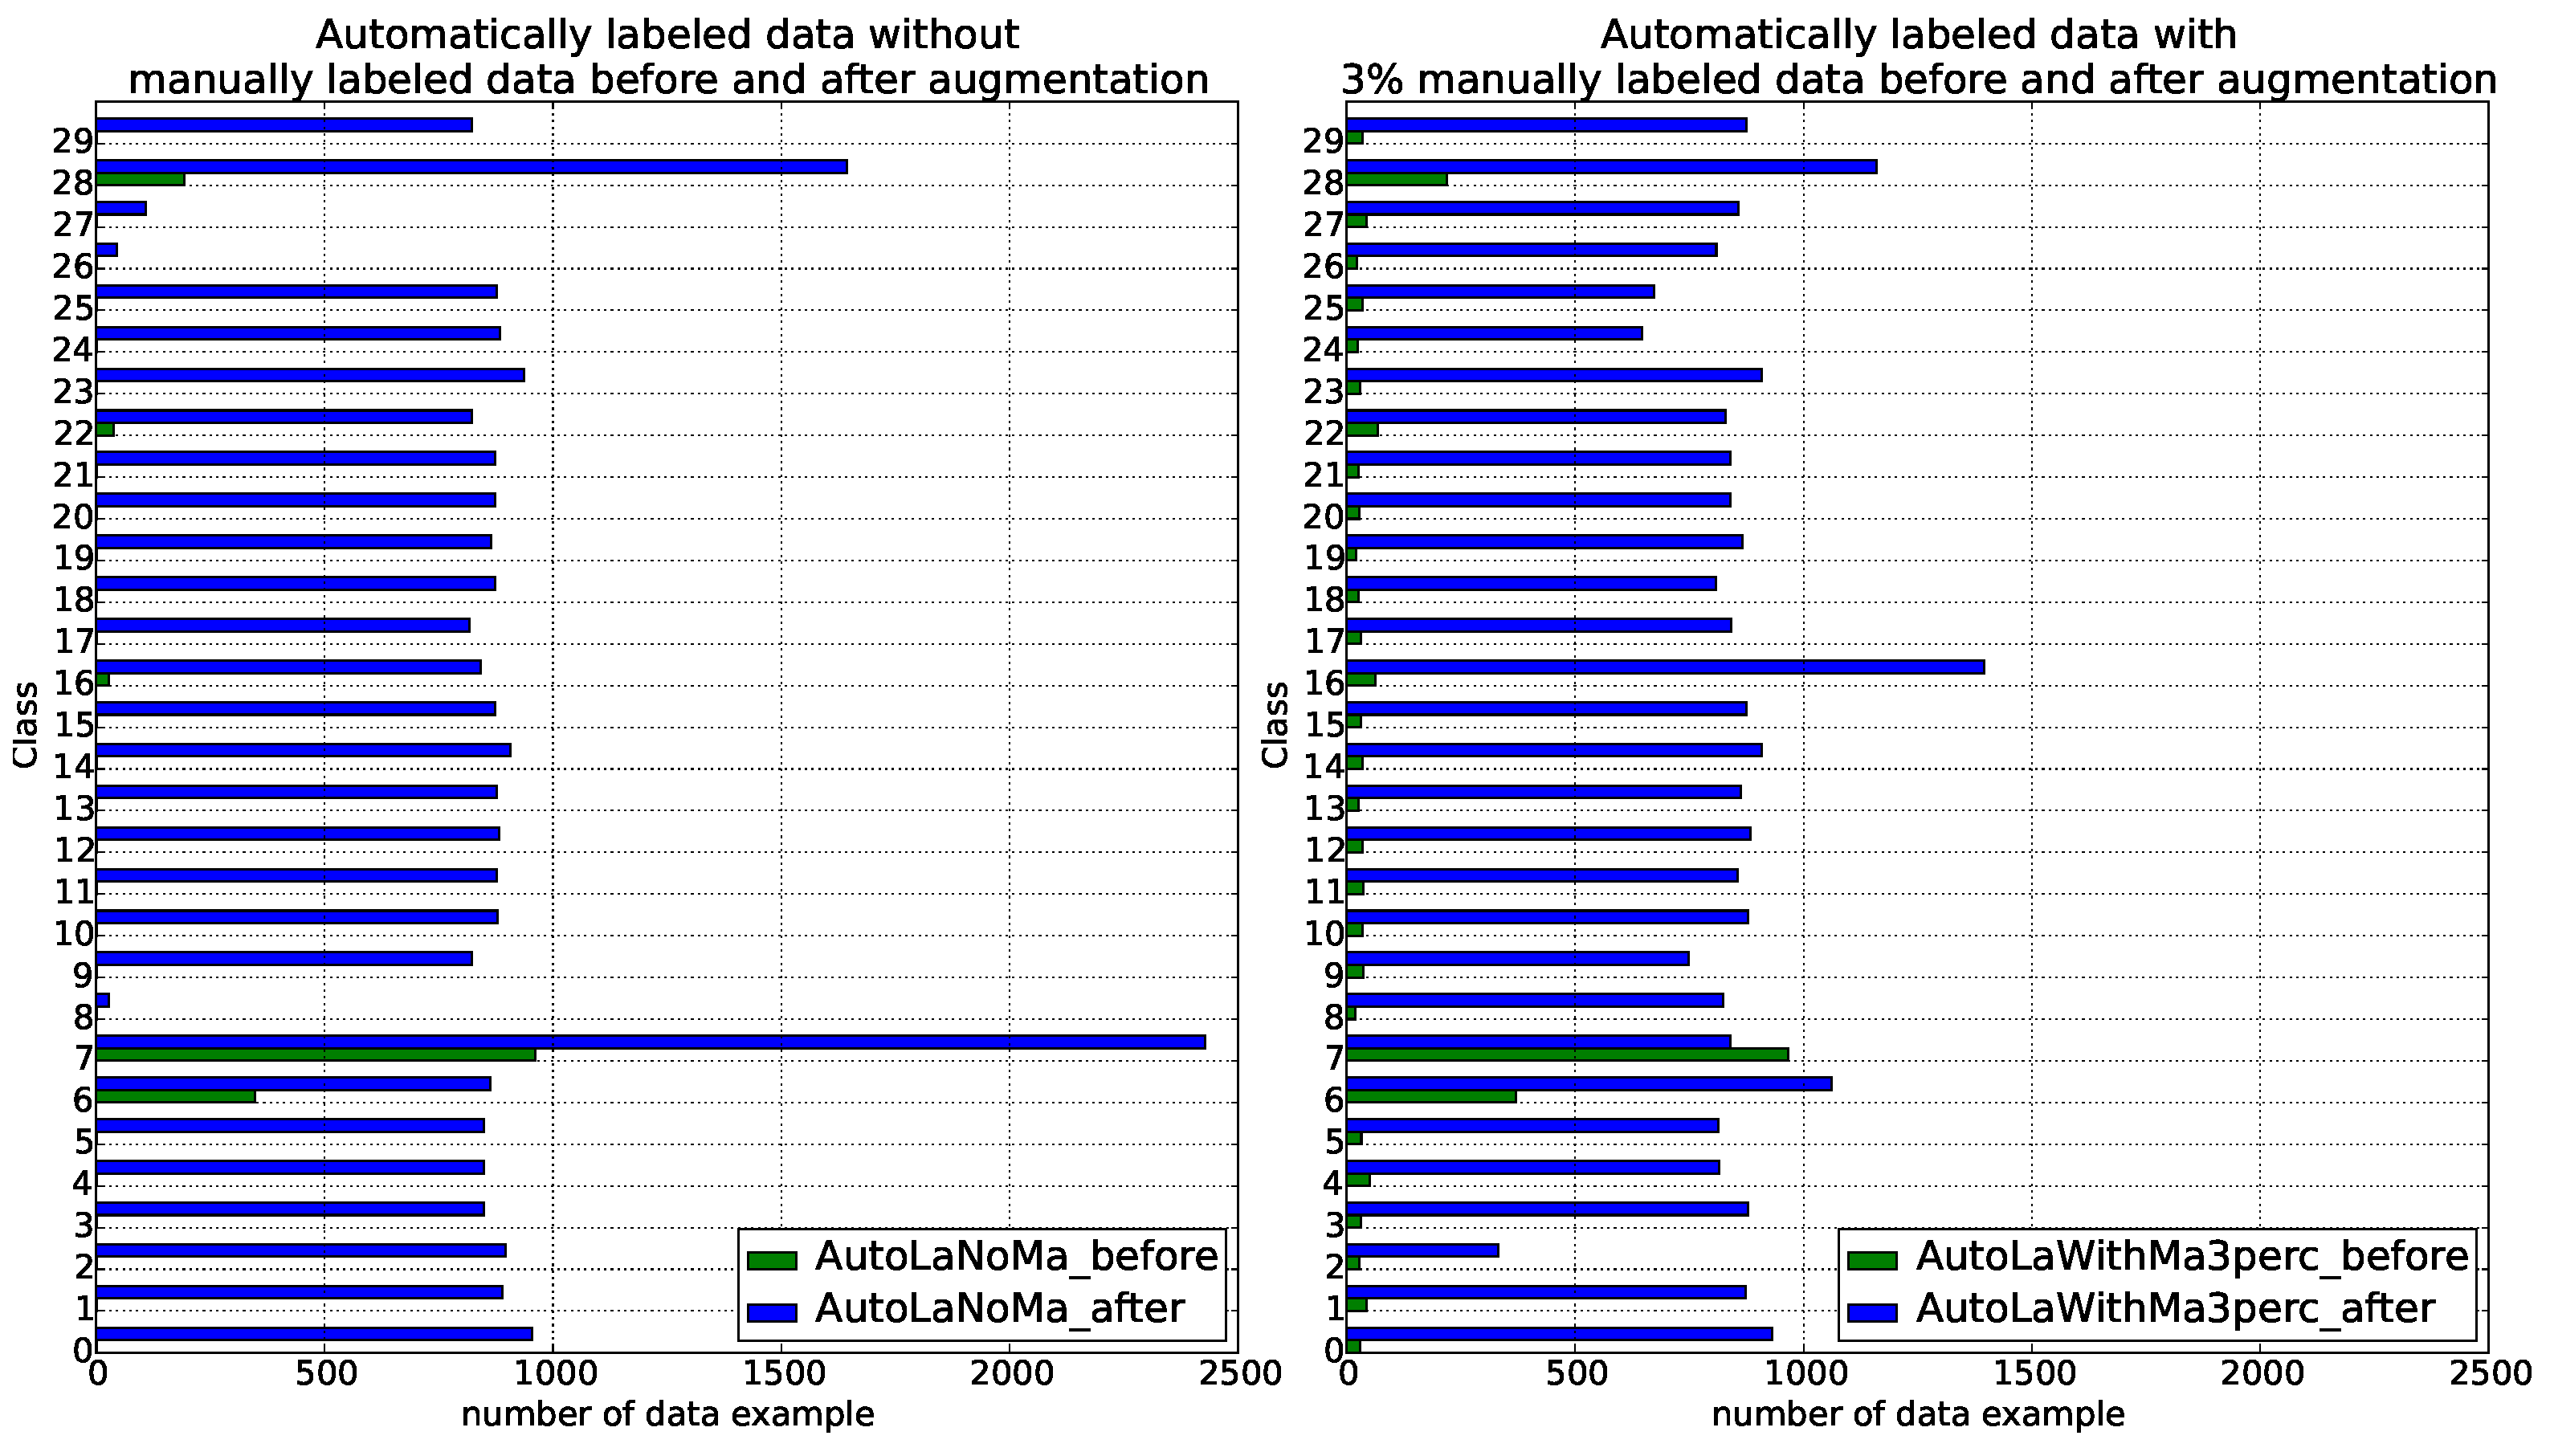
\includegraphics[height=9cm,width=15cm]{autoLa/exp2/class_balance_NoMa_3percMa.eps}
		\caption{Horizontal histograms of automatically labeled data with/without 3\% manually labeled data before/after augmentations.}		
		\label{hist_class}
	\end{center}
\end{figure}

\begin{figure}[H]
	\centering
	\begin{center}
		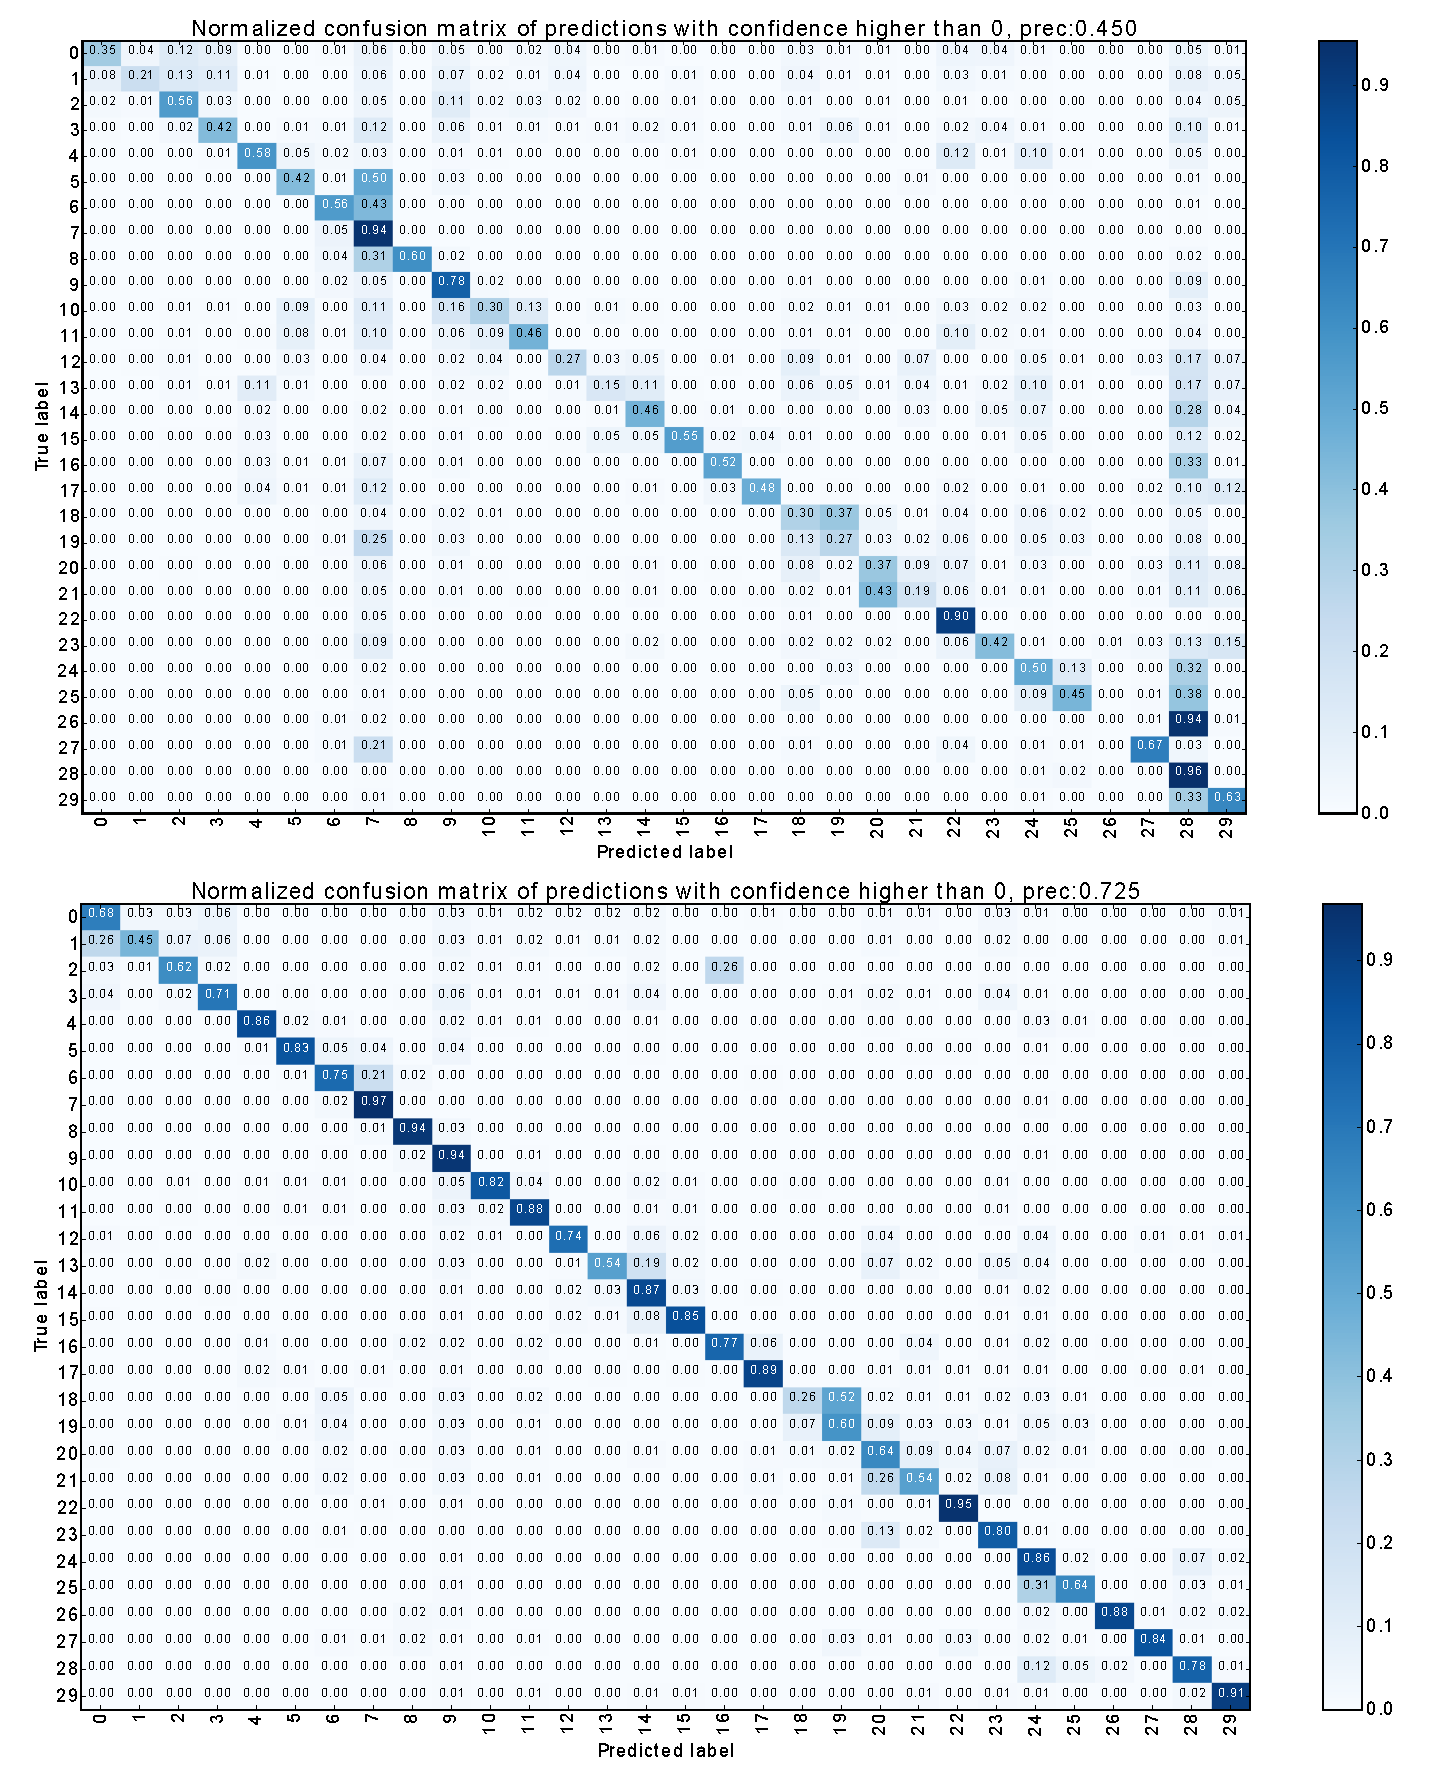
\includegraphics[height=15.5cm,width=13cm]{autoLa/exp2/AutoLaWithMa3perc&NoMa_CFM.eps}
		\caption{Confusion matrices of BNN fine-tuned with dataset with/without small portion of manually labeled data.}		
		\label{cfm_fine_tune_bnn}
	\end{center}
\end{figure}

%\begin{figure}[H]
%	\centering
%	\begin{center}
%		\includegraphics[height=9cm,width=16cm]{autoLa/exp2/AutoLaNoMa_FT_CFM.eps}
%		\caption{Confusion matrix of automatically labeled dataset(label index starts from 0).}		
%		\label{autoLa_exp2_cfm}
%	\end{center}
%\end{figure}
%
%\begin{figure}[H]
%	\centering
%	\begin{center}
%		\includegraphics[height=9cm,width=16cm]{autoLa/exp2/AutoLaWithMa3perc_CFM.eps}
%		\caption{Confusion matrix of automatically labeled dataset(label index starts from 0).}		
%		\label{autoLa_exp2_cfm}
%	\end{center}
%\end{figure}

%\begin{figure}[H]
%	\centering
%	\begin{center}
%		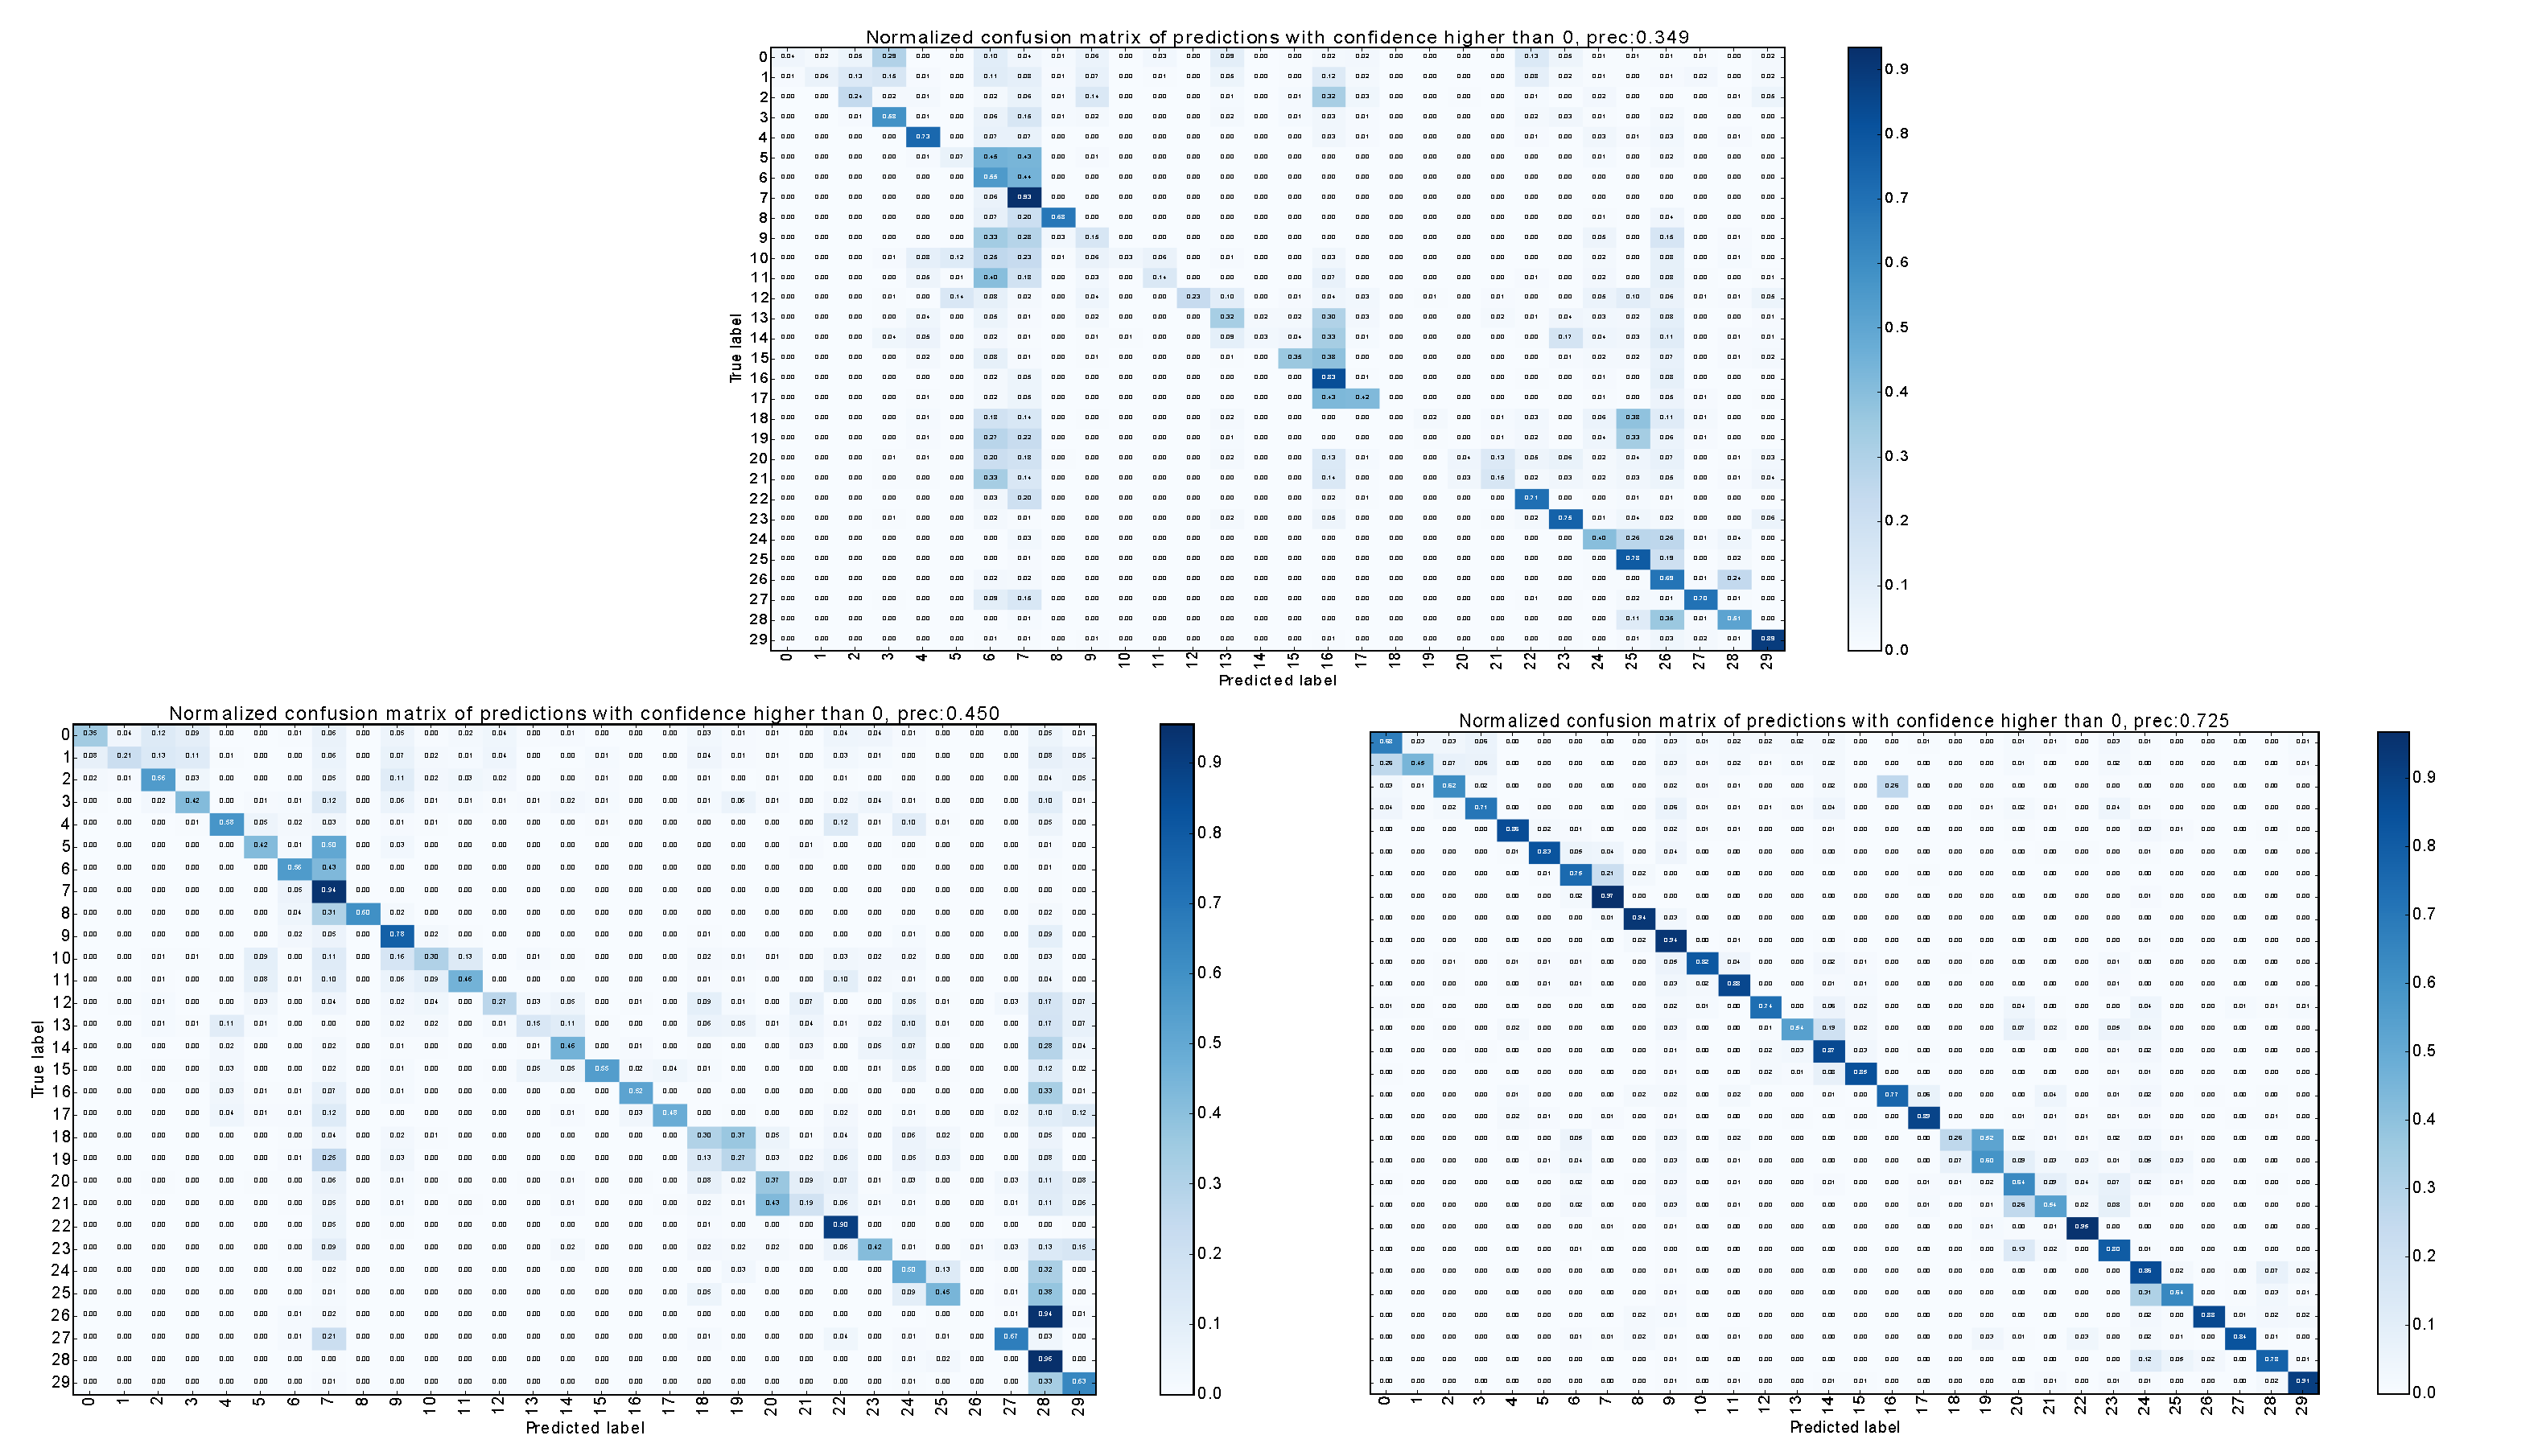
\includegraphics[height=10cm,width=16cm]{autoLa/exp2/all_CFMs.eps}
%		\caption{Confusion matrix of automatically labeled dataset(label index starts from 0).}		
%		\label{autoLa_exp2_cfm}
%	\end{center}
%\end{figure}

\section{Context-based improvement experiments}
In this section, experiments are performed to investigate the effect of combining improved uncertainty estimation with a probabilistic graphical model in down-stream task. In detail, we employ conditional random field (CRF) to capture the dependencies between objects by exploiting contextual information in the scene(cf. Fig.\ref{com_crf}). The intuition behind this idea is that, if the predictive distribution from BNN is more reliable and can represent the inherent randomness better. Then this bit of information can be utilized by CRF for further performance gain. Similar to previous experiments, ResNet50 with concrete dropout is used to improve uncertainty estimation in the following experiments and we call it \textbf{BNN} without specifications. 

Firstly a simpler experiment is performed on subset of T-LESS dataset to show that CRF can capture the dependencies and improve the accuracy, which can be boosted with better uncertainty estimation from BNN. Secondly, the same idea is tested on the entire T-LESS dataset to show the generalization ability of this approach. 


\subsection{Experiment \RNum{1}: evaluation on subset of T-LESS dataset}
In this experiment, original ResNet50 and BNN are trained on the real single objects with black background (original training set of T-LESS dataset). Then a subset of test scenes of original T-LESS dataset are used for training and testing CRF. In detail, scene 1, 2, 3, 4 ($\sim$8K objects and $\sim$2K scenes) are used for training CRF, and scene 5, 6, 7, 8 ($\sim$12K objects and $\sim$2K scenes) for testing. To note that \textbf{no augmentations} are applied in this experiment. To note that, based on the prior knowledge about the testing set, that no objects repeat in the test scenes, we set the diagonal entries of binary co-occurrence matrix with -1 to penalize the outcome with two same objects.

In the table \ref{table:crf_exp1_acc}, results of CRF trained with two different unary features from original ResNet50 and BNN are given. As can be seen, CRF trained and tested with unary feature from BNN can yield more improvement(13.17\%) compared with that from deterministic network (12.42\%).  

 \begin{table}[H]
 	\centering
 	\caption{Results of CRF trained with unary feature from different versions of ResNet50}
 	\label{table:crf_exp1_acc}
 	\begin{tabular}{|c|c|c|}
 		\hline
 		\multicolumn{1}{|l|}{}                                            & \begin{tabular}[c]{@{}c@{}}accuracy with\\ unary\\ potential\end{tabular} & \begin{tabular}[c]{@{}c@{}}accuracy with\\ unary and pariwise\\ potentials\end{tabular} \\ \hline
 		\begin{tabular}[c]{@{}c@{}}unary feature \\ from ori\end{tabular} & 48.79\%                                                                   & 61.21\%                                                                                 \\ \hline
 		\begin{tabular}[c]{@{}c@{}}unary feature \\ from BNN\end{tabular} & 51.94\%                                                                   & 65.11\%                                                                                 \\ \hline
 	\end{tabular}
 \end{table}

%When it comes to the advantage of modeling contextual information, it can be seen in figure \ref{cfm_crf_exp1}, in which confusion matrices of predictions from tests without and with CRF are listed. 

%\begin{figure}[H]
%	\centering
%	\begin{center}
%		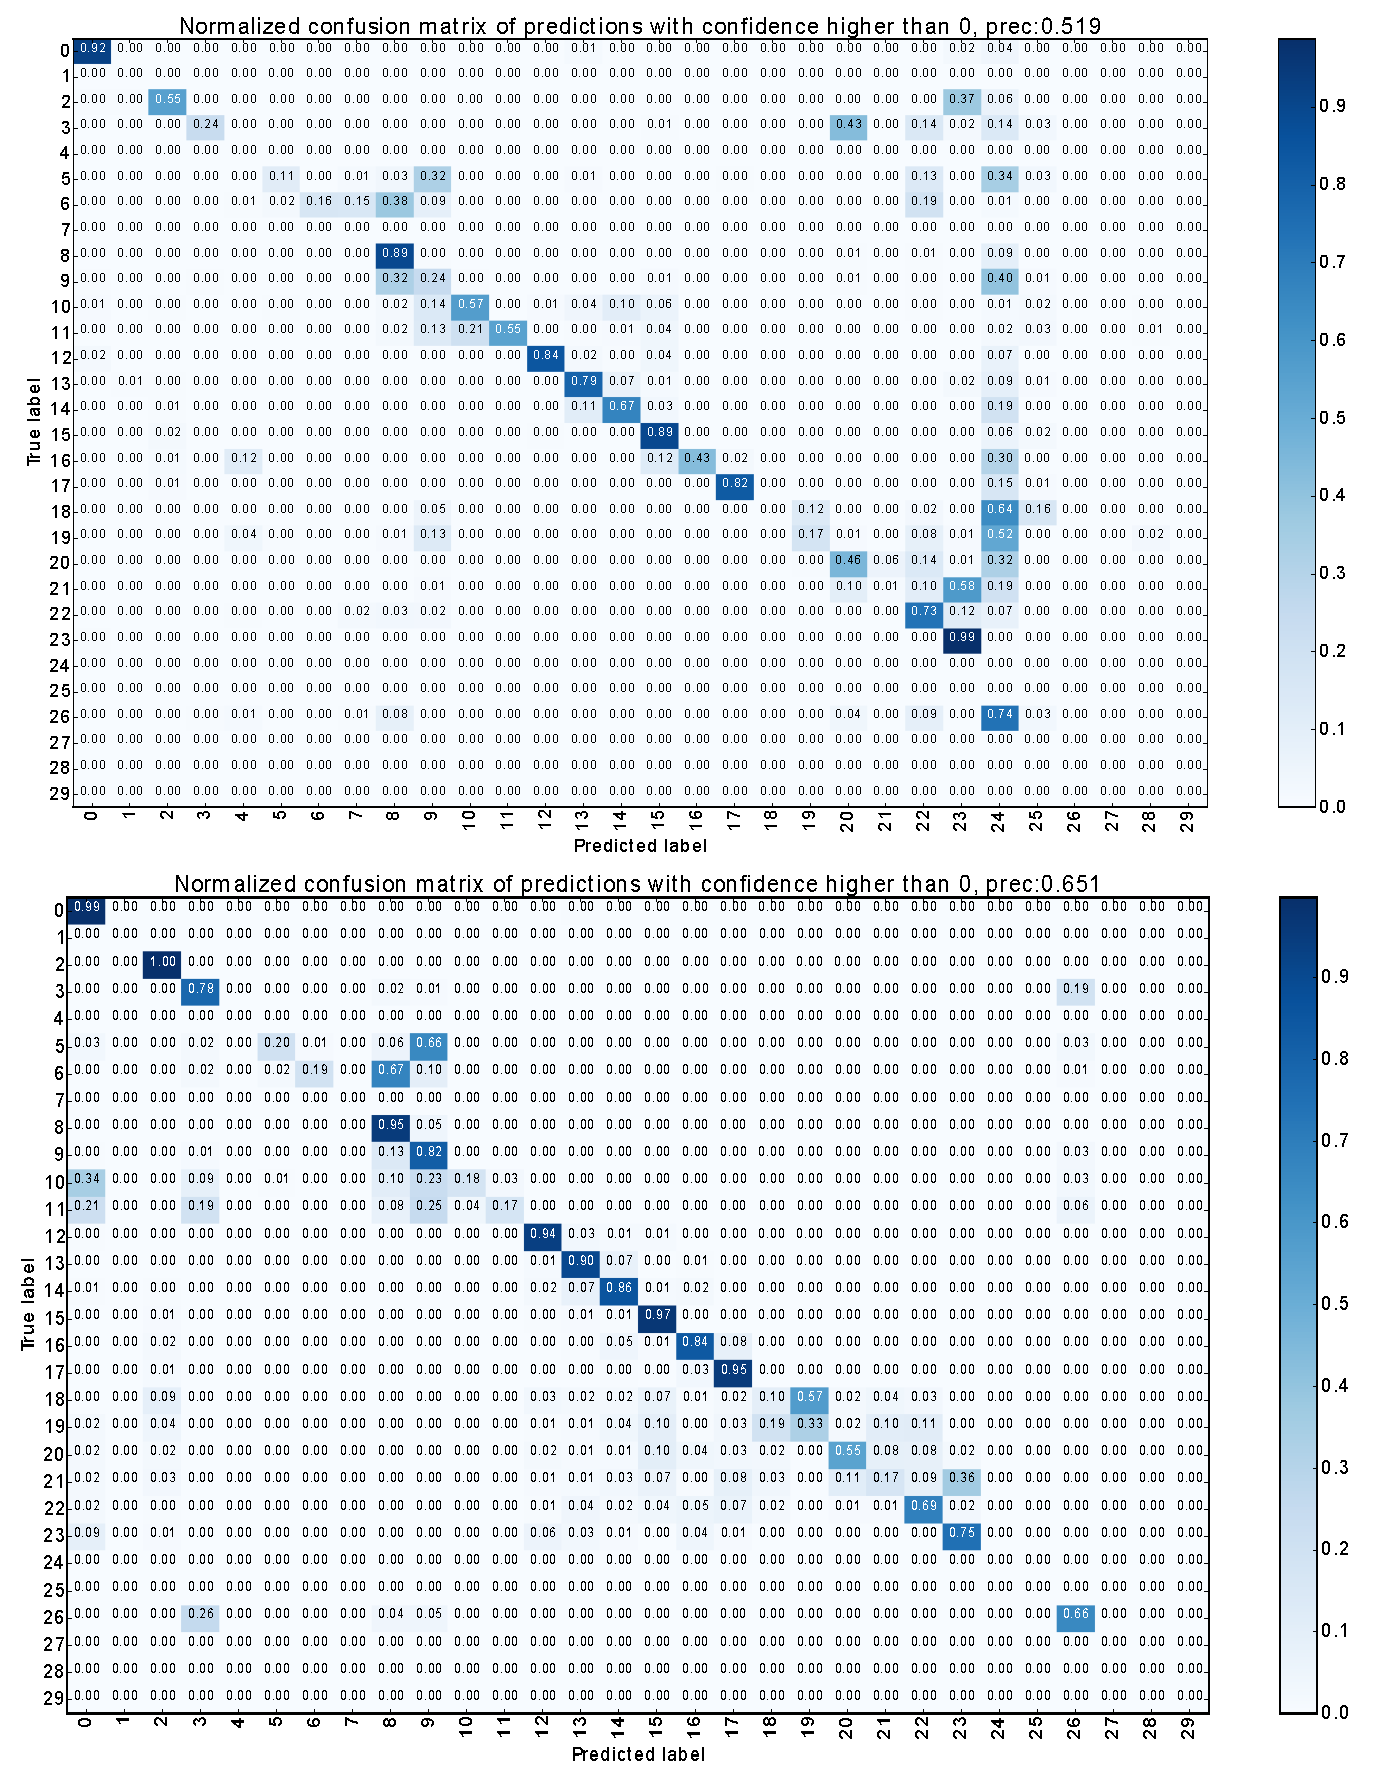
\includegraphics[height=16cm,width=13cm]{autoLa/exp2/bnn&bnncrf_test_scene5678.eps}
%		\caption{confusion matrices of predictions from tests without and with CRF.}		
%		\label{cfm_crf_exp1}
%	\end{center}
%\end{figure}
Additionally, because the weights in CRF model act as coefficients for two kinds of features, we can check the magnitude of these two weights for their contributions to overall performance. In the table \ref{table:crf_exp1_weights}, the weight of unary feature $\theta_u$ from BNN is larger than the one of edge feature $\theta_p$. The situation is inverse in unary feature from original ResNet50. It's evident that the unary feature from BNN contributes more than the pairwise one while the one from original ResNet50 contributes less. It also shows that the predictive distribution from BNN contains more information than its counterpart from original ResNet50. More importantly, this information can be utilized to improve the performance which is shown in the table \ref{table:crf_exp1_acc}.
\begin{table}[H]
	\centering
	\caption{Learned weights of CRF trained with unary feature from different versions of ResNet50}
	\label{table:crf_exp1_weights}
	\begin{tabular}{|c|c|c|}
		\hline
		\multicolumn{1}{|l|}{}                                            & \begin{tabular}[c]{@{}c@{}}node weight\\ $\theta_u$ \end{tabular} & \begin{tabular}[c]{@{}c@{}}edge weight\\ $\theta_p$ \end{tabular} \\ \hline
		\begin{tabular}[c]{@{}c@{}}unary feature \\ from ori\end{tabular} & 3.744                                                   & 4.213                                                   \\ \hline
		\begin{tabular}[c]{@{}c@{}}unary feature \\ from BNN\end{tabular} & 4.635                                                   & 3.882                                                   \\ \hline
	\end{tabular}
\end{table}

\subsection{Experiment \RNum{2}: evaluation on entire T-LESS dataset}
In this experiment, approach of combination of BNN and CRF is tested on the whole T-LESS dataset. Based on the results obtained in subsection \ref{con_learn_tless}, the accuracy should be improved further by exploiting contextual information with CRF (cf. Fig.\ref{fig:combined_crf}). In details, CRF are trained with unary features extracted from BNN before fine-tuning with size around $\sim$24.5 objects and $\sim$5K scenes (cf. Fig.\ref{fig:con_learn}). In testing, the whole testing set of original T-LESS dataset with size $\sim$70K objects and $\sim$10K scenes, whose unary features are extracted from fine-tuned BNN. 

Because the combinations of the whole test set are more complex than that of scene 5, 6, 7, 8 in experiment \RNum{1}, we try different values on the diagonal with which different prior knowledge is encoded. There are many objects occurring repeatedly in other scenes of test set besides scene 5, 6, 7, 8. Therefore there is a trade-off between different kind of prior knowledge. Filling diagonal entries with 1 indicates that co-occurrence of same objects is more likely to happen and it suits better on the whole test set. As can be seen in the table \ref{crf_exp2}, CRF trained with pairwise matrix with 1 on diagonal has most improvement (4\%) when comparing with matrices with other diagonal values.


\begin{table}[H]
	\centering
	\label{crf_exp2}
	\caption{Results of CRF with different type of potentials}
	\begin{tabular}{|l|c|}
		\hline
		Type of potential                                                              & \multicolumn{1}{l|}{Accuracy} \\ \hline
		Unary                                                                          & 72.48\%                       \\ \hline
		\begin{tabular}[c]{@{}l@{}}Unary and \\ pairwise(-1s on diagonal)\end{tabular} & 73.40\%                       \\ \hline
		\begin{tabular}[c]{@{}l@{}}Unary and \\ pairwise(0s on diagonal)\end{tabular}  & 74.64\%                       \\ \hline
		\begin{tabular}[c]{@{}l@{}}Unary and \\ pairwise(1s on diagonal)\end{tabular}  & 76.50\%                       \\ \hline
	\end{tabular}
\end{table}